\documentclass[11pt,a4paper,table]{beamer}
\mode<presentation>

\usepackage[spanish]{babel}
\usepackage[utf8]{inputenc}
\usepackage{amsmath}
\usepackage{amsfonts}
\usepackage{amssymb}
\usepackage{graphicx}

\usetheme[secheader]{Boadilla}
% diagramas temporales
\newcounter{wavecount}

\AtBeginSubsection[]
{
	\begin{frame}<beamer>{Agenda}
		\tableofcontents[sections=\thesection,currentsubsection]
	\end{frame}
}
\usepackage{siunitx}
%\usepackage{tabulary}
\usepackage{listings}
\usepackage{booktabs}
\usepackage{multirow}
\usepackage{pgfplots}
\usepackage{fancyvrb}
\usepackage{longtable}
\pgfplotsset{compat=1.3}
\usepackage{tikz}
\usetikzlibrary{arrows,babel,backgrounds,circuits.logic.US,decorations.pathreplacing,fit,patterns,petri,positioning,shapes,shapes.gates.logic,trees}

\newcommand\blfootnote[1]{%
	\begingroup
	\renewcommand\thefootnote{}\footnote{#1}%
	\addtocounter{footnote}{-1}%
	\endgroup
}

\tikzset{
	invisible/.style={opacity=0},
	visible on/.style={alt={#1{}{invisible}}},
	alt/.code args={<#1>#2#3}{%
		\alt<#1>{\pgfkeysalso{#2}}{\pgfkeysalso{#3}} % \pgfkeysalso doesn't change the path
	},
}

%\tikzstyle{style} = [definition]
\tikzstyle{interior}=[rectangle,rounded corners,draw=black,minimum size=3em, text width=20,fill=white]
\tikzstyle{exterior} = [rectangle,draw=black,minimum size=40]
\tikzstyle{mode text} = [midway,sloped,text width=200]
\tikzstyle{contenedor} = [rectangle,draw=black]
\tikzstyle{core}=[interior]
\tikzstyle{perif} = [interior,minimum height=20]
\tikzstyle{buf}=[core, text width=53, align=center]
\tikzstyle{obuf} = [buf, node distance=.7]
\tikzstyle{env} = [fill=black!20]
\tikzstyle{simple}=[rectangle, draw=black, minimum height=220, text width=65,align=center]
\tikzstyle{moore} = [rectangle,draw=black, minimum height= 30,text width=80,align=left]
\tikzstyle{mealy} = [rectangle,rounded corners=12, draw=black, text width = 80,align=left,minimum height=40]
\tikzstyle{ask} = [diamond,text width=50,draw=black,align=center,]
\tikzstyle{bloque}=[exterior,align=center,minimum size=60,text width=60]
\tikzstyle{hub}=[draw=black,anchor=west,circle]
\tikzstyle{dev}=[draw=black,anchor=west,rectangle,rounded corners,text width=60,align=center]
\tikzstyle{pid}=[draw=black,align=center,rectangle,rounded corners,minimum width=20,minimum height=110,pattern=north east lines,pattern color=black!35]
\tikzstyle{dir}=[draw,rectangle,rounded corners,minimum width=20,minimum height=110,align=center]
\tikzstyle{data}=[draw=black,align=center,rectangle,rounded corners,minimum width=80,minimum height=110,fill=black!05]
\tikzstyle{crc}=[draw=black,align=center,rectangle,rounded corners,minimum width=20,minimum height=110,pattern=dots,pattern color=black!25]
\tikzstyle{field}=[draw=black,rectangle,rounded corners, minimum height=30,align=center]
\tikzstyle{chart}=[circle,draw=black,text width=50,align=center]
\tikzstyle{lineaExt} = [->,line width=5pt, >=latex, shorten <= 1]
\tikzstyle{lineaInt} = [->,line width=3pt,white, shorten >= 4.8, >=latex, shorten <= 2]

\newcommand{\epg}[3]{
	Buffer {#1}\\
	[44pt]EP{#2}\\
	[44pt]{#3} Bytes}

\newcommand{\ep}[3]{
	Buffer {#1}\\
	[8pt]EP{#2}\\
	[8pt]{#3} Bytes}

\newcommand{\newwave}[1]{
	\path (0,\value{wavecount}) node[text width=45,anchor=east,align=right]{#1} node[coordinate](t_cur){};
	\draw (0,\value{wavecount}+.3) --++(.2,0);
	\draw (0,\value{wavecount}-.3) --++(.2,0);
	\path (t_cur) --++(.3,0)node[coordinate](t_cur){};
	\addtocounter{wavecount}{-1}}

\newcommand*{\bit}[2]{
	\draw (t_cur) -- ++(0.1,.6*#1-.3) -- ++(#2-.2,0) -- ++(+.1,.3-.6*#1)
	node[coordinate] (t_cur) {};}
%diagramas temporales
\newcommand*{\bitvector}[2]{
	\draw[] (t_cur) -- ++( .1, .3) -- ++(#2-.2,0) -- ++(.1, -.3)
	-- ++(-.1,-.3) -- ++(.2-#2,0) -- cycle;
	\path (t_cur) -- node[align=center] {#1} ++(#2,0) node[coordinate] (t_cur) {};}

\newcommand*{\graybitvector}[2]{
	\draw[fill=black!15] (t_cur) -- ++( .1, .3) -- ++(#2-.2,0) -- ++(.1, -.3)
	-- ++(-.1,-.3) -- ++(.2-#2,0) -- cycle;
	\path (t_cur) -- node[align=center] {#1} ++(#2,0) node[coordinate] (t_cur) {};}

\newcounter{wavecount}


\author[E. Barragán]{Edwin Barragán\\ \texttt{edwin.barragan@cab.cnea.gov.ar}}
\title{Temas Específicos de Electrónica Digital I}
\subtitle{Comunicación USB 2.0 para aplicaciones cientificas basadas en FPGA}
\institute[UNSJ-FI]{Universidad Nacional de San Juan\\Facultad de Ingeniería}
\setbeamertemplate{title page}{
\begin{center}
	\begin{beamercolorbox}[center,sep=3mm]{title}
		\textbf{\inserttitle} \par
		\carrera\\
	\end{beamercolorbox}
	\vfill
	\begin{beamercolorbox}[center,sep=3mm]{subtitle}
		\insertsubtitle
	\end{beamercolorbox}
	\vfill
    \parbox{100pt}{\centering \textbf{\insertauthor}}\\
      Autór\\
    \vspace{3mm}
	\parbox{.9\textwidth}{\centering \textbf{\asesores}}\\
	Asesores\\
	\vfill
	\parbox{.45\textwidth}{\insertinstitute}		
	\vfill
    {\centering \insertdate}
\end{center}
}

\begin{document}
%TODO tengo 18 filminas que no deben ser consideradas
	\titlepage
	\begin{frame}{Agenda}
		\tableofcontents[hideallsubsections]
	\end{frame}
	\begin{frame}{Agenda}
		\tableofcontents[sections={1,2}]
	\end{frame}
	\begin{frame}{Agenda}
		\tableofcontents[sections={3,4}]
	\end{frame}
	\section{Introducción}
		\framesubtitle{Preámbulo}
		\subsection{Objetivos}
			\begin{frame}{Objetivos}
	\begin{center}
		\only<1>{\begin{tikzpicture}[>=latex,scale=1.2]
				\begin{scope}[transform shape]
					\node[bloque](pc){PC};
					\node[bloque](adq)[right =3 of pc]{Sistema de adquisicíon basado en FPGA};
					\draw[<->,ultra thick]([yshift=5]pc.east) -- node (data)[above]{Datos} ([yshift=5]adq.west);
					\draw[<->,ultra thick]([yshift=-20]pc.east) -- node (ctrl)[above]{Control} ([yshift=-20]adq.west);
				\end{scope}
				\begin{scope}[on background layer]
					\node[rounded rectangle,fill=blue!20,fit=(pc.east)(adq.west)(data)(ctrl)]{};
				\end{scope}				
			\end{tikzpicture}}

		\only<2>{\begin{tikzpicture}[scale=.7,>=latex]
				\begin{scope}
					\begin{scope}[transform shape,node distance=2]
						\node[bloque] (cy) {Interfaz USB};
%						\only<3->{\node[bloque]	(cy)				{Interfaz\\\alert{Cypress FX2LP}};}
						\node[bloque]	(fpga)	[right=of cy]{FPGA};
%						\only<4->{\node[bloque]	(fpga)	[right=of cy]{FPGA\\\alert{Xilinx Spartan VI}};}
						\node[bloque]	(pc) 	[left=of cy]	{PC};
%						\only<5->{\node[bloque]	(pc) 	[left=of cy]	{PC\\\alert{libusb}};}
						\draw[->,thick] (pc.15) -- node (usbd+) [above]	{D+} (pc.15 -| cy.west);
						\draw[->,thick] (cy.195) -- node (usbd-) [below]	{D-} (cy.195 -| pc.east);
						\draw[<->,thick] (cy.15) -- node (data) [above] {Datos} (cy.15 -| fpga.west);
						\draw[->,thick]  (fpga.195) -- node (ctrl) [below] {Control} (fpga.195 -| cy.east);
						\node[node distance=.4,text=blue] (usb text) [above=of usbd+] {USB};
					\end{scope}
					\begin{scope}
						\node[rectangle,rounded corners,draw=blue,dashed,fit=(usb text)(usbd+)(usbd-)(cy.south west)(pc.east)](usb){};
					\end{scope}
				\end{scope}
			\end{tikzpicture}}
	\end{center}


	\begin{itemize}
		\only<1>{\item Objetivo General
				\begin{itemize}
					\item Realizar una comunicación entre un FPGA y una PC mediante USB 2.0.
				\end{itemize}}
		\only<2>{\item Objetivos Particulares
				\begin{itemize}
					\item Seleccionar la interfaz USB.
					\item Comprender el funcionamiento del kit de desarrollo CY3684 utilizado como interfaz USB y el framework provisto por Cypress.
					\item Realizar la configuración de la interfaz USB.
					\item Sintetizar un circuito en VHDL que sea capaz de interactuar con la interfaz USB.
					\item Sintetizar circuitos de prueba para realizar una verificación funcional.
					\item Validar el funcionamiento.
				\end{itemize}}
	\end{itemize}
\end{frame}

		\subsection{Motivación}
			Un carpintero desea medir la distancia de una barra de madera que luego será, tal vez, la altura de las patas de una futura mesa. Para ello, utiliza una cinta métrica, compuesta de una cinta metálica que posee una escala graduada. Sabe entonces que la barra mide la distancia que coincide con la distancia de la cinta graduada.\\

Un panadero desea medir cuanto pesa la harina que debe para poder amasar. Entonces, la coloca en una balanza y observa cuanto marca su indicador. Así conoce que la masa de la harina es equivalente a la fracción de medida que indica la balanza.\\

Un atleta desea conocer cuanto demora en correr un trayecto que posee \SI{1.00}{\kilo\meter}. Por esto, registra el valor que indica su reloj al principio del recorrido y cuando alcanza el final observa nuevamente el artefacto. Luego de esto, calcula la diferencia entre el valor final y el inicial, conociendo cuanto tiempo le tomó realizar su travesía.\\

En los tres casos anteriores, tanto el carpintero, como el panadero y el atleta desconocen algo y necesitan cambiar su estado con respecto a esa incertidumbre. Por ello recurren a diferentes objetos, a fin de obtener conocimiento a partir de ellos. Sin embargo, estos objetos, por si mismos, no otorgan información, sino más bien otorgan un dato, que comparado y contrastado con otros datos, se traducen en conocimiento.\\

La información es el resultado de recopilar, ordenar y procesar un conjunto de datos, de forma tal que permitan adquirir mayor conocimiento sobre un asunto determinado y otorguen un significado mayor que cada uno de los datos por separado. En el caso del carpintero, compara el tamaño de las patas de la mesa con una cinta metlálica, que a su vez, posee registrada su distancia en función de algún patrón de metrología, establecido por convención. Esto quiere decir que el dato 1, la longitud del patron, junto al dato 2, escala graduada de la cinta, más el dato 3, la longitud de la cinta métrica, permiten al carpintero cambiar su estado de desconocido a conocido, con respecto a la longitud del trozo de madera, a través de la información proporcionada por el conjunto de datos.\\

Se puede realizar el mismo análisis con respecto a la balanza del panadero, considerando un peso patrón, un desplazamiento y una escala graduada o una señal eléctrica emitida por una celda de carga deformada un porcentaje de su capacidad, registrada previamente por su fabricante conforme a pesos patrones, y un circuito adaptador que transforma esa señal electrica en un valor numérico mostrado en un indicador.\\

El atleta compara las posiciones y los desplazamientos de las agujas de su reloj, previamente calibrado para que dé una vuelta por cada minuto en una aguja, otra aguja que dé una vuelta por hora y la tercera una vez cada 12 horas. Además, es probable que él haya ajustado la hora que indica el reloj para que otorgue un horario idéntico al de referencia, establecido por convención.\\

En todos los casos, se recopila una gran cantidad de datos que, ordenados, procesados y comparados otorgan al usuario una utilidad mayor que la del dato en sí, ya sea una longitud, una masa, un tiempo o cualquiera sea la variable física que se desee conocer.\\

La Ciencia es un conjunto de técnicas y procedimientos que, a través de un método científico, busca adquirir, descubrir y/o desarrollar nuevo conocimiento. Se desprende entonces, que la ciencia produce, de forma fundamental, datos, que luego de un procesado se transforman en información. A su vez, el estudio detallado de esta información genera conocimiento.\\

Cuando se nombra la palabra ciencia, se hace referencia a un conjunto conformado por diferentes objetos de estudio. El objeto de estudio es el sujeto a través del cuál se da la principal clasificación de las diferente ramas de la Ciencia: las Ciencias Sociales estudian las relaciones humanas y las Ciencias Naturales dedican sus esfuerzos a objetos que se encuentran en la naturaleza. Dentro del último grupo encontramos las Ciencias de la Tierra se enfocan en una rama más particular de la naturaleza, como lo es el estudio de la superficie terrestre; y siguiendo así se puede encontrar muchas más clasificaciones de ciencias, incluso como ramas englobadas por las anteriormente nombradas.\\

Sin embargo, la producción científica necesita adquirir una gran cantidad de datos que luego serán ordenados, procesados, analizados y transformados en información y conocimiento. En este sentido, la incorporación de una herramienta especialmente diseñada para el procesamiento de datos, como lo es la computadora, permite manejar un numero creciente de información. Es por eso que se encuentra en desarrollo un gran número de sensores y dispositivos que permitan obtener flujos crecientes de datos.\\

Uno de los desarrollo que se encuentra actualmente en boga es el de sensores y sistemas que adquieran imágenes de diferentes tipos. La captura de imágenes requiere de sistemas digitales de alta velocidad que tengan la capacidad de acarrear los datos desde el lugar físico en donde se obtienen los datos, es decir, en el transductor mismo, hasta el circuito o el sistema destinado al proceso de los mismos.\\

Para este tipo de aplicaciones, se torna de interés la utilización de un tipo particular de dispositivos electrónicos denominados FPGA ({\it Field-Programmable Gate Array}, o en español, Arreglo de Compuertas Programables en Campo), circuitos integrados programable para sintetizar circuitos digitales de alta velocidad. En otras palabras, este tipo de componentes permite implementar circuitos que ejecutan tareas complejas y resuelve problemas específicos.\\

Existen numerosos trabajos que utilizan FPGA para la producción de imágenes. Por ejemplo, el desarrollo de un sensor de radiación utilizando un sensor CMOS comercial. Para ello, los autores utilizaron un FPGA para configurar y transmitir imagenes a un grabador de video a través de puerto UART. Esto permitió adquirir una imagen a través de un disparador realizado con un pulsador\cite{Perez2017}.\\

Se denomina ultrasonografía a la técnica de adquirir imágenes basandose en rebotes de ultrasonido. Sus aplicaciones son múltiple, en las que se destaca el diagnóstico médico, ya que es una técnica no invasiva y sin riesgos de radiación ionizante sobre el paciente. Un trabajo reciente desarrolló un sistema de ecografía médica con bajo costo utilizando un FPGA\cite{biswas2018embedded}. El autor también presentó un algoritmo realizado y probado en PC. Luego se implementó e en una FPGA.\\

Existen sistemas de telescopía implementados con FPGA. Yanagisawa y otros desarrollaron un sistema con telescopios pequeños para explorar objetos de campo cercano con la finalidad de monitorear cuerpos celestes que puedan colisionar con el planeta\cite{Yanagisawa2018}. Los autores utilizan la velocidad de los circuitos implementados en FPGA para minimizar el tiempo de adquisición.

Existen sensores de imagenes de distancia desarrollados mediante FPGA\cite{Cui2018}.\\%BORRAR esta cita!!!

A diferencia de un microprocesador o un microcontrolador, también muy usados en la industria electrónica, en el cual una unidad logica algoritmica ejecuta un programa cargado secuencial, es decir, linea por línea, un FPGA puede ser programado de forma tal que cada proceso se ejecute en forma independiente y paralela, dotando al sistema de una mayor velocidad en el procesamiento.\\

De esta forma, un diseñador puede manipular un volumen mucho mayor de datos, que a los efectos de la adquisición y medición de imágenes, resulta más adecuado.\\

Pero como ya se mencionó con anterioridad, la obtención de datos por si misma no le otorga al científico la información, y por ende, el conocimiento nuevo que desea. Para ello, es probable que este gran flujo de datos requiera de un procesamiento y análisis más exhaustivo de los mismos.\\

Es por esto que la PC {\it Personal Computer} se ha transformado en la herramienta indispensable en cualquier ámbito, pero en especial en los entornos en donde se requiere el  manejo, cálculo, procesamiento y análisis de grandes cantidades de datos e información.\\

Se torna de suma utilidad, entonces, proveer una comunicación efectiva y robusta que permita mover grandes volúmenes de datos en poco tiempo, y de esta forma facilitar los tiempos de desarrollo, las pruebas y depuración de sistemas.\\

Desde la inclusión de la norma USB, en el año 1996 a la fecha, se ha convertido en el elemento que no falta en ningun equipo, al punto tal que ha desplazado a cualquier otro conector. Al punto tal es esto, que para requerir algún puerto adicional que no sea de esta norma, cualquier comprador debe especificar que así sea, mas no es necesario especificar que tiene USB como norma de conexión.\\

El presente trabajo pretende ofrecer una comunicación basada en la versión 2.0 de la norma USB entre una PC y un FPGA, y otorgue una herramienta adicional a científicos que desarrollen o utilicen sistemas basados en FPGA.\\
%
%Este trabajo, pretende elaborar una interfaz entre los dos extremos, es decir, entre la PFGA y la PC, de forma tal que permita a un desarrollador, investigador o usuario en general, obtener una comunicación confiable y con un ancho de banda que permita mover el flujo de datos que genera una sensor que adquiera imágenes.\\
%
%Es cierto que el protocolo puede ser totalmente implementado en una FPGA, sin embargo, esto requeriría un muy alto costo tanto económico como en recursos disponibles del chip programable para una tarea genérica que es mejor elaborar con un circuito integrado diseñado especialmente para tal fin. Es por esto que se utiliza como lazo de interfaz un chip comercial elaborado por Cypress Semiconductor.\\
%
%
%
%[1][https://ieeexplore.ieee.org/abstract/document/8214376]
%[2][http://www.idr.iitkgp.ac.in/jspui/bitstream/123456789/9068/1/NB15975_Abstract.pdf]
%[3][https://ieeexplore.ieee.org/abstract/document/8396725]




%El mundo actual, en el que vivimos inmersos, demanda y consume volumenes cada vez más grandes de información. Con solo hacer una rapida miradad en diarios, incluso no especilizados, se observa la importancia que poseen las ciencias y disciplinas que manejas la informacion, aquellas areas agrupadas dentro del conjunto Técnico de la Información y la Comunicación, o más ocnocido por sus siglas, TIC's.
%
%Internet de las cosas , Big Data, Inteligencia Artificial, Redes Neuronales, Robótica, Domótica, entre otras, son areas en las que los datos y la información es abultada y su correcto manejo es sumamente complejo e importante. Además, ninguna de las actividades científicas, puede escapar de esta gran demanda mundial de información.
%
%La información es un conjunto de datos ordenados y procesados de forma tal que permita al que lo lea que eleve su nivel de conocimiento sobre un determinado tema. Es decir que, para que exista información, en primer lugar tenemos que tener datos, de forma tal que podamos luego procesarlos y obtener realmente información de llos.
%
%Como ejemplo de esto, podemos citar simplemente el acto de medir la presión dentro de un tubo de gas. Sería normal pensar en que, teniendo este objetivo en mente, simplemente coloquemos un manómetro en la salida del tubo. El manómetro es un artefacto que posee una varilla 
%
%
%
%
%
%El mundo, durante la era de la información, nos exige producir y consumir cada vez más y más información. En cada aspecto social dela vida de la persona se pueden encontrar ejemplos claros de esto.\\
%
%Bajo un punto de vista social nos vemos bombardeados por información. Los 'influencers' que se mueven a traves de Facebook, Twiter, Instagram, Snapchat, Linkedin, Youtube, etc, necesitan para estar a la moda, producir constantemente material y que ese material sea consumido por alguien que este demandando esa información.
%
%En el area de econimía y finanzas existen cada vez más robots que extraen información de las diferentes bolsas, periodicos, bancos, industrias y donde se ocurra que pueda haber información útil, para tomar mejores decisiones que, por supuesto, también ejecutan los robots.
%
%En el comercio, desde las tiendas de supermercado hasta las tiendas digitales que trabajan solo a través de internet están constantemente recabando datos y procesandolos a din de diseñar estrategias que permitan ofrecer productos que se adapten mejor a lo que busca el cliente y de esa forma lograr vender mayores volumenes.
%
%La industria cuenta cada vez más con multiplicidad de posibilidades basadas en sensores que adquieren grandes cantidades de datos que son almacenadas y procesadas, muchas vecen 'en línea' o 'al instante', de forma tal de encontrar mejores procesos o ejecutar nuevas tareas, como por ejemplo la industria automotriz, enfocada cada vez más en autos que puedan manipular todo el entorno y ser totalmente autónomos de un conductor.
%La industria espacial y satelital dotan a sus equipos de mayores sensores y mayores flujos de datos. La industria médica brinda cada vez más posibilidades de diagnóstico a traves de nuevas técnicas y formas de adquisición de imágenes.
%
%A todo esto, la ciencia y el desarrollo de nuevas aplicaciones y equipos, no son indiferente. Cada vez se encuentran más innovaciones y desarrollos de nuevos sensores que adquieren flujos de información crecientes. La toma de imagenes se ha vuelto una herramienta clave para la investigación en diversas areas, tales como la biología, la ciencia de materiales, las ciencias nucleares, las ciencias de la tierra, etc.
%
%Las redes sociales son un ejemplo de esto, pero esto se observa en la industria, la economía, las finanzas e incluso hasta en la casa.
%
%
%
%[1] file:///home/lechuzin/Facultad/Trabajo%20Final/lechuzing/docs/bibliografia/The-Rise-of-the-Network-Society-With-a-New-Preface-Volume-I-The-Information-Age-Economy-Society-and-Culture-Information-Age-Series-.pdf
		\subsection{Bus Serial Universal}
			El Bus Serial Universal, o USB por sus siglas en inglés, es un sistema de comunicación diseñado durante los años 90 por seis fabricantes vinculados a la industria informáticas, Compaq, Intel, Microsoft, Hewlett-Packard, Lucent, NEC y Philips, con la idea de proveer a su negocio de un sistema que permita la conexión de PCs con teléfonos y periféricos con un formato estándar, fácil de usar y que permita la compatibilidad entre los distintos fabricantes.\\

Hasta ese momento, el gran ecosistema de periféricos, sumado a los nuevos avances y desarrollos, hacia muy compleja la interoperatividad de todos ellos. Cada uno de los fabricantes desarrollaba componentes con características, tales como fichas, niveles de tensión, velocidades, drivers, lo cuál dificultaba al usuario estar al día y poder utilizar cada componente que compraba. Esto también complicaba a las mismas empresas productoras, por que la introducción de un nuevo sistema requería de mucho soporte extra para poder conectar todo lo ya existente.\\

Todo esto, quedó saldado con el aparición de la norma USB que, gracias a la gran cuota de mercado de sus desarrolladores, fue adoptado en forma rápida y se transformó en la especificación por defecto a la hora de seleccionar un protocolo. Al punto tal esto se cumplió que hoy, más de 20 años después, es muy difícil encontrar PC's con otro tipo de puertos, salvo que, en el momento de su compra, se solicite especialmente un puerto determinado. Así, cualquier PC nueva disponible en el mercado debe poseer puertos USB para la conexión de los periféricos.\\

El diseño de la norma USB busca resolver tres problemáticas interreacionadas, que son: La conexión de teléfonos con las PC, la facilidad de uso, es decir, que el usuario solo conecte su dispositvo y pueda utilizarlo, y la expansión en la cantidad de puertos disponibles para conectar periféricos\cite{USBspec}. Para satisfacer estas tres demandas, la norma USB 2.0 busca alcanzar un conjunto de metas que apuntan a la facilidad del uso, la compatibilidad entre versiones diferentes de la misma tecnología, la robustez en el flujo de datos, y la convivencia de diferentes configuraciones temporales en único bus, provistos de una interfaz estándar, ancho de banda que soporte comunicaciones audiovisuales de calidad aceptable y un bajo coste.\\

El presente capitulo intenta ser un breve resumen con los aspectos más relevantes de la norma en cuanto a su composición física, su topología, los dispositivos que intervienen, la importancia de los mismos y como los datos son transmitidos desde y hacia una PC.\\

%	Desde el punto de vista técnico, el protocolo USB es un sistema del tipo maestro-esclavo, donde el maestro, denominado {\it HOST}, debe ser necesariamente una PC (o un dispositivo con software y hardware capaces de incorporar los drivers necesarios) y cualquier periférico a ella acoplada será un esclavo\cite{USBspec}.\\
%	
%	Para describirlo es conveniente diferenciar tres partes. Una capa física, en donde se definen los componentes que intervienen, una capa de protocolo, en donde se define el formato, el marco en el que son enviados los paquetes, como se direccionan y como se comunican entre sí, y una parte lógica, en donde cada componente es visto solamente como un extremo y define como fluyen los datos desde un extremo hacia la PC y viceversa.\\
%	
%	\subsection{Capa física}
%		
%	\begin{figure}[!ht]
%		\centering
%		\begin{tikzpicture}[scale=1.2\textwidth/\paperwidth,>=latex]
%			\begin{scope}
%				\begin{scope}[transform shape,node distance=2,grow=right,sibling distance=80, level distance=30]
%					\node[draw=black] (host) {\it HOST}
%						child {node[hub] (root) {Raiz} edge from parent[level distance=70,<->]
%							child{node[hub](hub){HUB} edge from parent [<->,sibling distance=35,level distance=50]
%								child {node	[dev]	(out){Función} edge from parent [<-]}
%								child {node	[dev]	(in){Función} edge from parent [->]}
%								child {node (text) {Dispositivo compuesto} edge from parent [draw=black!0]}
%							}
%							child{node[dev]{Función} edge from parent [->]}
%							child{node[dev]{Función} edge from parent [<-]}
%						};
%				\end{scope}
%				\begin{scope}
%					\node[draw=black,rounded corners, dashed, fit=(hub)(out)(in)(text)]	(comp)	{};
%				\end{scope}
%			\end{scope}
%		\end{tikzpicture}
%		\caption{Topología de un sistema USB}
%		\label{fig:arqusb}
%	\end{figure}
%		
%	En esta sección no se describirán los detalles de las conexiones eléctricas ni mecánicas a las que se refieren las especificaciones de la norma USB debido a dos cuestiones fundamentales. Una de ellas es que toda esta sección de la norma está resuelta ya por los fabricantes de la interfaz que se utiliza en este trabajo. A su vez, maneja todas las señales, arma y desarma los paquetes que salen hacia la PC y que llegan de ella respectivamente. Por otro lado, no es el objetivo de este trabajo adentrarse en esos detalles. Gracias a la extensión de este tipo de comunicación existen una gran cantidad de fabricantes en el mercado que fabrican cada uno de los componentes, ya sean, cables, conectores en todas sus versiones, adaptadores de un tipo de estos, su costo es despreciable con respecto a cualquier tipo de desarrollo en ese sentido y son de una muy buena calidad, es decir que todos cumplen con lo que la norma establece. Sí, se describen los dispositivos físicos y su categoría, según la norma, en función del rol que cumplen.\\
%	
%	La comunicación USB posee una topología maestro-esclavo. Es decir, existe un dispositivo que dirige todas las transferencias de datos y otros que responden a sus directivas. Por esto, el elemento central de cualquier comunicación USB es el {\it HOST} (director o anfitrión, por su traducción de la voz inglesa). Él es el que posee el {\it Host USB Controller}\cite{USBspec}. Esto quiere decir que tiene la capacidad de registrar los dispositivos acoplados, asignarles dirección, colocar los paquetes de salida y/o llegada en sus respectivas listas y servilos a los procesos que utilizan esta comunicación. Además, el {\it HOST} se encarga de enviar los tokens a todos los periféricos, con la dirección del dispositivo, el sentido de la comunicación, el tipo de transferencia que se espera y todas las acciones de control que el sistema requiera. En la mayoría de los casos, el {\it HOST} es una PC, auqnue también puede ser cualquier dispositivos  ``inteligente'' como un smartphone.\\
%	
%	En el otro extremo de la comunicación, se encuentran lo que la norma denomina {\it funciones}\cite{USBspec}. Las {\it funciones} son todos los periféricos que actúan como fuente o sumidero de información. Es decir, en caso de periféricos de entrada, serán una fuente de datos hacia el {\it HOST}. Si los periféricos son de salida, serán un sumidero de la información que proporciona la PC. Los casos de periféricos de entrada/salida, se denominan {\it dispositivos compuestos}.\\
%		
%	Existe también, a los fines de la norma,un elemento intermedio, denominado {\it HUB} (concentrador o distribuidor, según la traducción del inglés). Este dispositivo se encarga de conectar dos o más {\it funciones}, ya sea de entrada o salida, de recibir y enviar las direcciones y de regenerar las señales que el {\it HOST} envía y deben ser recibidas por las {\it funciones}.\\
%	
%	La Figura \ref{fig:arqusb} muestra la topología típica de un sistema USB. En ella, se observa el {\it HOST} como un rectángulo, las {\it funciones} como rectángulos con los bordes redondeados y los distribuidores como círculos. Se puede notar que el {\it HOST} posee un distribuidor propio llamado {\it Raiz} en el cual se conectan todos las {\it funciones} y distribuidores. Cada {\it Función}posee una única dirección. Pueden existir dispositivos que posean funciones diversas con un mismo encapsulado, como por ejemplo un auricular que tenga micrófono incorporado. Este dispositivo, tendrá un {\it HUB} que concatena dos {\it funiones} diferentes.\\
%	
%	\subsection{Capa lógica}
%	Desde el punto de vista lógico, cada dispositivo es visto por el {\it HOST} como un extremo (EP, del inglés, {\it endpoint}) independiente, que posee solo un modo de comunicación, es decir, el protocolo se comunicara solo por un tipo de transferencia y en un único sentido con cada {\it EP}. En otras palabras, USB registra un periférico de entrada/salida como un {\it EP} de entrada y otro de salida en forma independiente.\\
%	
%	Esta independencia brinda la posibilidad de configurar cada extremo de forma diferente y obtener el ancho de banda necesario para la subida y bajada de datos, los tiempos de acceso al bus, la dirección y todo lo relacionado a los modos de comunicación conforme a los requerimientos.\\
%	
%	El protocolo entiende que entre le {\it HOST} y cada uno de los extremos existe un tubo (la norma en ingles habla de {\it pipes}) en donde la información es colocada y transferida. Luego, cada tubo posee la configuración establecida por el controlador del {\it HOST} y se comunica con cada {\it EP} por medio de estos tubos. A los fines del usuario, esto es lo importante, por cuanto se solicita acceso al bus y define en que buffer va a contener los datos a enviar o transmitir y el protocolo se encarga de el empaquetado, el armado de los cuadros, el acceso el bus y el posterior envío de datos.\\
%	
%	\subsection{Capa de protocolo}
%	En la capa de protocolo, la especificación de la norma detalla cómo se compone un cuadro y cómo deben ser estructurados los paquetes para que sean efectivamente enviados a través del sistema. Cada mensaje que se intercambia por el bus se denomina paquete. Cada paquete puede poseer hasta cinco campos, dependiendo del tipo de paquete que sea enviado a través del sistema y de quien sea el remitente. A su vez, cada paquete comienza con una señal de sincronismo ({\it SYNC}) y un Comienzo de Paquete (SOP de {\it Start-of-Packet}), y terminan con una señal de Fin de Paquete (EOP por {\it End-of-Packet}).\\
%	
%	Por otra parte, los paquetes está temporalmente encapsulados en cuadros. Cada cuadro posee un Comienzo de Cuadro (SOF, {\it Start-of-Frame}) y posee una duración de \SI{1}{\milli\second}, hasta el próximo SOF. En las comunicaciones de alta velocidad, es decir, aquellas que poseen una tasa de bit de \SI{480}{\mega\bit\per\second}. Se subdivide un cuadro en 8 micro-cuadros de \SI{125}{\micro\second} cada uno.\\
%	
%	\subsubsection*{Campos de Paquetes}
%	Cada paquete contiene un campo denominado identificador de paquete (PID del inglés {\it Packet Identifier}). El PID indica el tipo de paquete que se está enviando y, como consecuencia, el formato de cada uno, es decir, que campos acarrea y que control de datos utiliza.
%	
%	A su vez, cuando el host solicita algo al sistema, lo realiza a través del denominado campo de dirección. Este campo, se compone de dos partes, la primera es el campo de dirección de la función y el segundo es la dirección de extremo.\\
%	
%	Los mensajes de datos, poseen un campo dedicado de forma específica a los datos. Puede poseer un numero entero de bytes, desde \SI{0}{} a \SI{1024}{}.\\
%	
%	Para corroborar el envío de datos, USB utiliza verificación de redundancia cíclica (CRC o {\it Cyclic Redundancy Checks}). Los paquetes especiales y los de token poseen un verificador  CRC5, es decir, de 5 bits, cuyo polinomio generador es:
%	
%	\begin{center}
%		\begin{math}
%			G(X) = X^5 + X^2 + 1
%		\end{math}
%	\end{center}	
%	
%	Por su parte, los paquetes de datos, poseen CRC16, ya que pueden llegar a ser bastante extensos. En su caso, el polinomio generador está dado por:
%	
%	\begin{center}
%		\begin{math}
%			G(X) = X^{16} + X^{15} + X^2 + 1
%		\end{math}
%	\end{center}
%	
%	Existe un campo relativo a los cuadros temporales, que se denomina campo de número de cuadro. Este es enviado por el {\it HOST} en cada SOF y es incrementado a cada cuadro. Los micro-cuadros también poseen un número de cuadro, sin embargo, este es aumentado solamente cada 8 micro-cuadros, es decir, el número se incrementa cada \SI{1}{\milli\second} y se repite durante los 7 micro-cuadros de \SI{125}{\micro\second}, en comunicaciones de alta velocidad.\\
%	
%	\subsubsection*{Formato de paquetes}
%	
%	%TODO quedé por acá..
%	\begin{figure}[t]
%		\centering
%		\begin{tikzpicture}[scale=\textwidth/\paperwidth,>=latex]
%			\begin{scope}
%				\begin{scope}[transform shape,node distance=.15]
%					\node[pid]	(pidtok)	{P\\I\\D\\\ \\T\\o\\k.};
%					\node[dir]	(adtok)	[right=of pidtok]	{D\\i\\r.};
%					\node[dir]	(eptok)	[right=of adtok]	{E\\x\\t\\r.};
%					\node[crc]	(crc5)	[right=of eptok]	{C\\R\\C\\5};
%				\end{scope}
%				\begin{scope}
%					\node[exterior,minimum size=0,inner sep=1,fit=(adtok)(eptok)](tokad){};
%					\node[below=.01 of tokad.south,align=center,transform shape] (texttok){Paquete\\Token};
%					\node[exterior,inner sep=1,fit=(pidtok)(tokad)(crc5)(texttok)](pkttok){};
%				\end{scope}
%				\begin{scope}[transform shape,node distance=.15]
%					\node[pid,node distance=.4]	(piddat)	[right=of crc5]{D\\a\\t\\a\\\ \\P\\I\\D};
%					\node[data]	(data)	[right=of piddat]	{Datos\\útiles};
%					\node[crc]	(crc16)	[right=of data]	{C\\R\\C\\1\\6};
%				\end{scope}
%				\begin{scope}
%					\node[below=.01 of data.south,align=center,transform shape] (textdat){Paquete\\de Datos};
%					\node[exterior,inner sep=2,fit=(piddat)(data)(crc16)(textdat)]{};
%				\end{scope}
%				\begin{scope}[transform shape,node distance=.15]
%					\node[pid,node distance=1.5]	(hspid)	[right=of crc16]{H\\S\\\ \\P\\I\\D};
%				\end{scope}
%				\begin{scope}
%					\node[below=.01 of hspid.south,align=center,transform shape] (texths){Paquete\\de Handshake};
%					\node[exterior,inner sep=2,fit=(hspid)(texths)]{};
%				\end{scope}
%			\end{scope}
%		\end{tikzpicture}
%		\caption{Distintos tipos de paquetes USB}
%		\label{fig:usbpkts}
%	\end{figure}
%	
%	\begin{itemize}
%		\item {\bf Paquetes Token:} A través de este tipo de paquetes el host envía las directivas a los distintos periféricos. Estas directivas pueden ser IN, cuando solicita datos de un periférico; OUT, cuando se dispone a enviar datos hacia una {\it función}; SOF, que indica el inicio de cada cuadro, para que cada función se sincronice y SETUP, cuando va a enviar un paquete de configuración a algún extremo.
%		\item {\bf Paquete de Datos:} Este tipo de PID puede ser emitido por un dispositivo, si es que envía datos al host o bien por el mismo host cuando el flujo de datos es a la inversa.
%		\item {\bf Paquete de {\it Handshake}:} Es enviado por el receptor del mensaje y le informa al emisor el estado de la transferencia. ACK significa que el paquete fue recibido sin errores; NAK, los datos poseen error o el emisor no puede enviar; la señal STALL quiere decir que la solicitud no es soportada o que el extremo está detenido; NYET implica que no hay respuesta aún por parte del receptor.
%		\item {\bf Paquetes Especiales:} Son paquetes con propositos específicos. Con ellos se señalan preambulos emitidos por el {\it HOST}, se informan errores, se solicitan mensajes divididos en diferentes paquetes y se intercambia señales de ping para conocer el estado de los componentes del sistema.
%	\end{itemize}
%	
%	Cada uno de los tipos de paquetes posee un formato específico, tales como se muestran en la Figura \ref{fig:usbpkts}. En ella se observa que los paquetes de token envían un PID, una dirección y un CRC5; los paquetes de datos, se componen de un PID, los datos transmitidos y un CRC16; en el caso de los paquetes de Hanshake, solo el PID indica que tipo de mensaje se envía. Los paquetes especiales no se detallan ya que el formato es muy variable, en función del paquete.\\
%	
%	\subsection{Flujo de datos}
%	Como se menciono anteriormente, el host envía un toquen SOF que sirve para sincronizar los dispositivos al bus. En un sistema USB, el host provee la base de tiempo y envía cada \SI{1}{\milli\second} un SOF (Start of frame, o su traducción, inicio de cuadro) seguido de un numero de 11 bits que sirve para contar cada uno de los marcos. Además, en sistemas de alta velocidad, cada cuadro se divide en ocho microcuadros de \SI{125}{\micro\second}, que también son marcados por un SOF, sin embargo, el contador no se actualiza por cada microcuadro.\\
%	
%	Luego de esto, el sistema puede comenzar con la transferencia de datos. USB dispone 4 tipos de posibles transferencias, que se detallan un poco más adelante, y que pueden ser usadas conforme a los diferentes requerimientos del sistema.\\
%	
%	Cada transferencia de datos está compuesta por un primer paquete de token, emitido por el host, que posee el tipo de transferencia que se espera, sea de entrada, de salida, de control o especial; la dirección de la función que debe responder o recibir el mensaje enviado por el bus y los verificadores CRC5.\\
%	
%	Luego, el siguiente paquete posee los datos que se transfieren, precedido por un PID de datos, y verificadores CRC16. Este paquete es transmitido por el emisor de los datos. Finalmente, el receptor devuelve un paquete de {\it handshake}, indicandole al emisor si el transferencia fue efectiva o no.\\
%	
%	\subsubsection*{Transferencias por paquetes (Bulk transfers)}
%		Este tipo de transferencias puede ser dispuesta para trasmitir un gran flujo de datos. No posee perdida de datos gracias a un sistema de chequeo y retransmisión de datos. El inconveniente que presenta este tipo de transferencias es que en un nivel de prioridades se presenta en el final del sistema. Es decir, el bus solo va a ser usado para transferir este tipo de datos siempre que se encuentre desocupado, o bien, se le asignará una proporción ínfima de ancho de banda para poder trasnmitir con este modo. Es comunmente usado para trasmitir datos que no son críticos en tiempo, por ejemplo para scanners e impresoras.\\
%	
%	\subsubsection*{Transferencias de interrupción}
%		Este tipo de transferencias sirve para enviar y recibir paquetes de datos que requieren un buen sistema de control de errores, pero que, son más restrictivos en tiempos. El sistema siempre destinará un intervalo fijo de tiempo para transmitir los datos que estén pendientes para trasnferencias de interrupción.\\
%	
%	\subsubsection*{Transferencias Isocrónicas}
%		Este tipo de transferencias está destinado a datos que son críticos en tiempo. Es usado, principalmente para enviar datos ``a chorro'', como ser el caso de {\it streaming} de audio o video, en donde los datos producidos deben ser rápidamente llevados al usuario.\\
%	
%		No posee un control de errores muy sofisticado, más que un simple código CRC, pero no existe mecanismo de retransmisión de datos ni handshake entre los {\it EP} y el {\it HOST}.\\
%	
%		Como el tiempo es el requerimiento crítico en este tipo de datos, el controlador le asigna una determinada cantidad de tiempo de bus, o en otras palabras, una determinada cuota de ancho de banda.\\
%	
%	\subsubsection*{Transferencias de control}
%		Este tipo de transferencias solo las emite el host y el sistema las utiliza para configurar cada dispositivo. Debido a su criticidad, el controlador dispondra encada cuadro de una fracción de ancho de banda para las trasnmisiones de control. Es el tipo de transferencias que posee el sistema de detección de errores más sofisticado, de forma tal de asegurar la integridad de los datos de control.\\
%	
%		A cambio de esto, solo muy poca información puede ser trasmitida por cada cuadro, de hasta 64 bytes en sistemas de alta velocidad.\\


	\section{Implementación}
		\subsection{Arquitectura del sistema}
			\begin{figure}[hb]
	\centering
	\begin{tikzpicture}[scale=\textwidth/\paperwidth]
		\begin{scope}[>=latex, node distance=1, align=center, transform shape]
			\node	(aux1)	[]	{};
			\node[core,	minimum height=95]
					(mis)	[left=of aux1,anchor=north east]	{MIS};
			\node[core]	(ram)	[right=of aux1,anchor=north west, text width=30]	{16 kB RAM};
			\node[perif,text width=60]
					(xcvr)	[left=of mis]	{Transceptor USB};
			\node[interior,	minimum size=60, text width=50]
					(uc)	[above=of aux1]	{8051 Mejorado};			
			\node[perif,
			node distance=2.9]
				(pll)	[left=of uc]	{PLL};		
			\node	(aux2)	[right=of ram.south]{};				
			\node[core,	text width=120]
				(bus)	[right=of aux2,rotate=90,anchor=north west]	{Bus de datos y direcciones};		
			\node[perif]	(i2c)	[right=of bus.south east,anchor=north west]	{I2C};
			\node[perif,text width=30]
				(gpif)	[right=of bus.south west,anchor=south west] {GPIF};
			\node[perif,text width=40]
				(fifo)	[below=of gpif]	{4 kB FIFO};
			\node	(aux3)	[right=of fifo]	{};
			\node	(aux5) 	[left=of ram] {};
			\draw[<->]	(mis) -- (xcvr);
			\draw[<->]	(ram) -- (ram -| mis.east);
			\draw[<->]	(fifo) -- (fifo -| mis.east);
			\draw[<->]	(ram) to (ram -| bus.north);
			\draw[<->]	(uc) to (uc -| bus.north);
			\draw[<-]	(xcvr) to (xcvr |- pll.south);
			\draw[->]	(pll) to (uc);
			\draw[<->]	(i2c) to (i2c -| bus.south);
			\draw[<->]	(gpif) to (gpif -| bus.south);
			\draw[]		(fifo) -| (aux5.center);
		\end{scope}
	
		\begin{scope}[on background layer]
			\node[contenedor] (fx2) [fit=(pll)(xcvr)(uc)(bus)(mis)(ram)(fifo)(gpif)(i2c)(aux3)]{};
		\end{scope}
		
		\begin{scope}[transform shape,>=latex]
			\node[text width=40,align=center]	(xtal)	[left=of pll]{Xtal \SI{24}{\mega\hertz}};
			\node	(host)	[left=3of xcvr]	{PC};
			\draw[<->,ultra thick] (host) -- node [above,text width=70,midway,align=center]{Comunicación USB} (xcvr);
			\draw[->] (xtal) to (pll);
			\draw[<->,ultra thick] (bus.240) -- node [above,align=center,text width=80] {Datos, direcciones y entradas adicionales}(bus.240 -| fx2.east);
			\draw[<->,thick] (gpif) to (gpif -| fx2.east);
			\draw[<->,thick] (fifo) to (fifo -| fx2.east);
			\draw[<->,thick] (i2c) to (i2c -| fx2.east);
		\end{scope}
	\end{tikzpicture}
	%		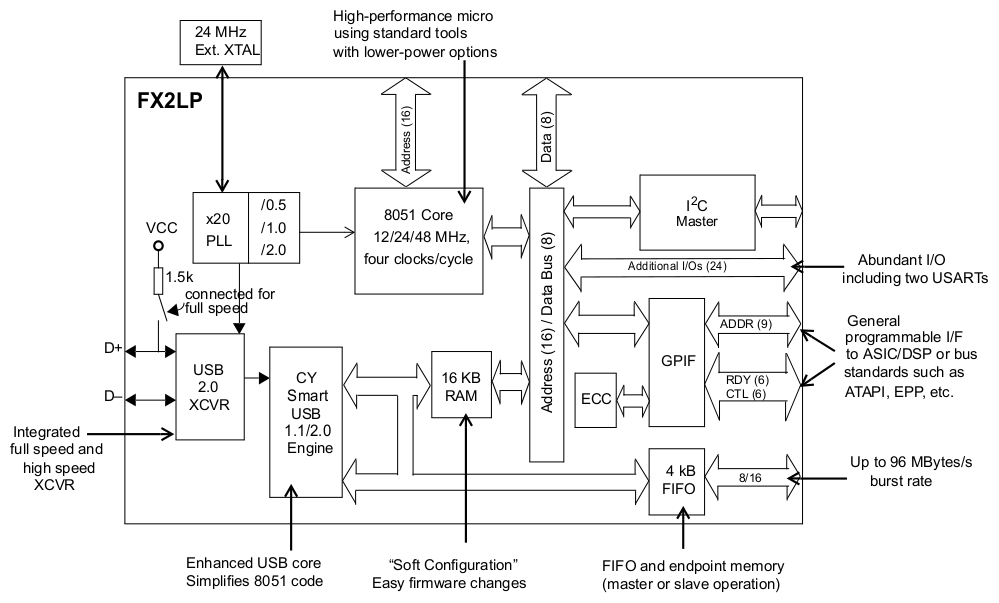
\includegraphics[width=.7\textwidth]{arqfx2lp.png}
	%		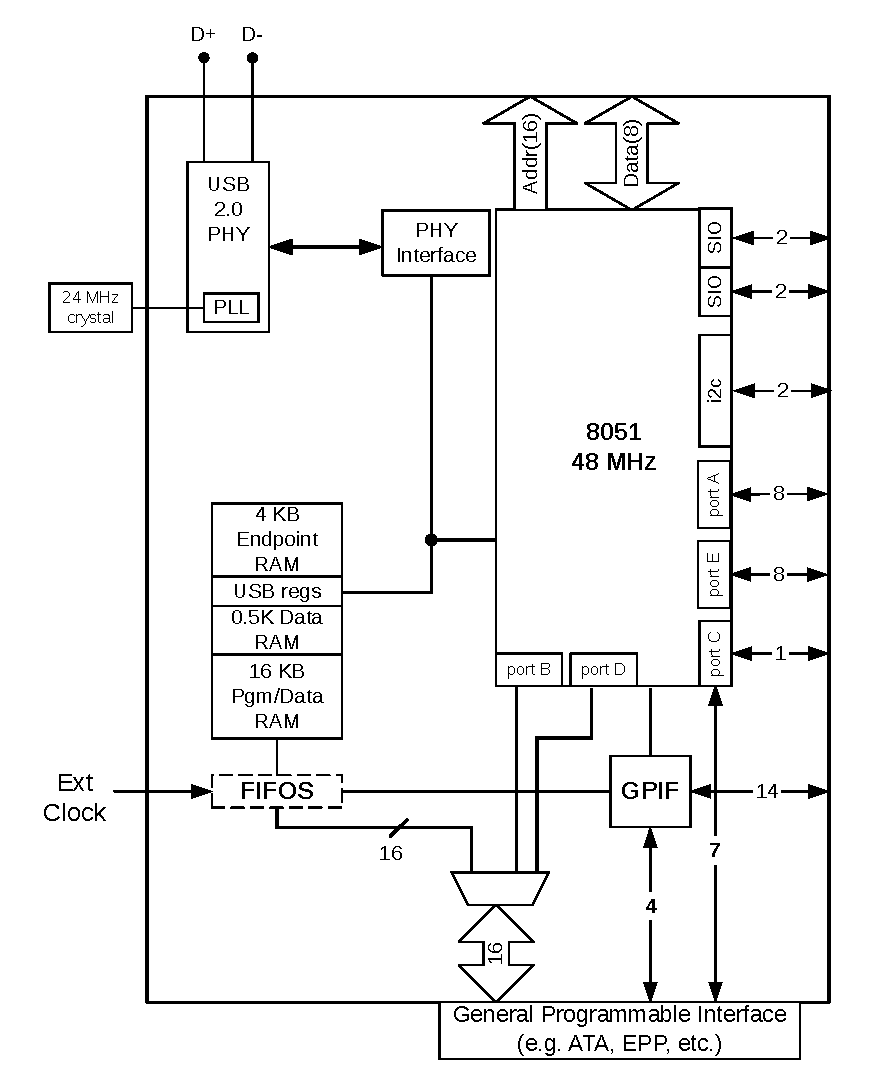
\includegraphics[width=.55\textwidth]{arq.eps}
	\caption{Arquitectura FX2LP} 
	\label{arqEzUSB}
\end{figure}

El núcleo del kit de desarrollo CY3684 es el controlador EZ-USB FX2LP. La serie de controladores FX2LP se caracteriza por brindar una conexión USB 2.0 de alta velocidad y bajo consumo energético. Está diseñada, preferentemente más no exclusivamente, para periféricos que se alimentan a baterías y poseen una autonomía energética limitada.

La arquitectura de controlador FX2LP, tal como se presenta en la Figura \ref{arqEzUSB}, integra un controlador USB completo, es decir, incluye un transceptor USB, un Motor de Interfaz Serie (MIS) y buffers configurables para datos. Incorpora también una versión del microcontrolador ($\mu$C) Intel MCS-51, más conocido como el $\mu$C 8051, que contiene registros y funciones adicionales orientadas a mejorar el rendimiento de la comunicación USB y memoria RAM de \SI{16}{\kilo\byte} de capacidad, para almacenar programas y datos. 
%Cypress agrega, como interfaz programable hacia los periféricos, una memoria tipo FIFO (\(First In First Out\); Primero Entrado, Primero Salido) con una capacidad de \SI{4}{\kilo\byte} que es operada en modo esclavo (es decir, necesita un dispositivo que le provea la lógica para operar) y destinada a almacenar datos de la comunicación, una interfaz de propósito general (GPIF) y un puerto I$^2$C. Además posee un PLL con divisor configurable a través del cual provee las señales de reloj adecuadas para el correcto funcionamiento del sistema.%\\
El modelo del flujo de datos posee dos extremos entre las cuales el controlador cumple el rol de interfaz. Estos extremos son la PC y el FPGA respectivamente. El controlador necesita, entonces, poder comunicarse tanto con el Host como con los periféricos. Para este propósito, Cypress agrega al circuito integrado del controlador dos puertos USART ((acrónimo de Transmisión y Recepción Asíncrona en Serie Universal, en inglés)), una interfaz de propósito general (GPIF), un puerto I$^2$C y una memoria FIFO (\(First In First Out\); Primero Entrado, Primero Salido).

La GPIF está pensada principalmente para poder utilizar sistemas que deban ser comandados en forma externa, como por ejemplo un registro de desplazamiento. Por su parte, la memoria FIFO posee \SI{4}{\kilo\byte} de capacidad reservados para almacenar los datos que se intercambian y se destina a aquellos sistemas que pueden proveer las señales de control, aunque también puede ser comandada por el GPIF. Con estas interfaces se posibilita la conexión con casi cualquier dispositivo, ya sea estandarizado (ATA, PCMCIA, EPP, etc) o personalizable (DSP, FPGA, $\mu$C);

%El usuario puede trasmitir datos desde y hacia el Host a través del mismo puerto USB. Sin embargo, también posee dos puertos USART ((acrónimo de Transmisión y Recepción Asíncrona en Serie Universal, en inglés)) que permiten comunicarse con la PC y facilitan en gran medida la tarea de depuración del desarrollo.

%En cuanto a la interfaz con uno o mas periféricos, el controlador posee un puerto $I^2C$, una interfaz de propósito general (GPIF), para sistemas que necesitan ser comandados en forma externa; y una interfaz con memorias FIFO esclavas, a través de las cuales se puede conectar sistemas que cumplen un rol activo en el envío y recepción de información. Estas tres interfaces posibilitan la conexión de dispositivos que poseen tanto puertos estandarizados (ATA, PCMCIA, EPP, etc.), cómo personalizables (DSP, FPGA, microcontroladores, etc).

%Variante 1
 
%El usuario puede trasmitir datos desde y hacia el anfitrión a través del mismo puerto USB, o bien via RS-232. Para comunicarse con sistemas periféricos se puede aprovechar el puerto $I^2C$, la interfaz de propósito general, que actúa como maestro y a la cual se le puede acoplar un periférico esclavo, y/o las memorias FIFO en modo esclavo que puede ser conectada a un sistema maestro. Esto brinda muchas alternativas, desde la conexión a puertos estandar, como ser ATA, PCMCIA, EPP, etc. o también la conexión de dispositivos tales como DSP's y FPGA's.\\
%\textbf{\hl{variante 1}}
%\hl{El usuario puede trasmitir datos desde y hacia el anfitrion a traves del mismo puerto USB, o bien via RS-232. Para comunicarse con sistemas perifericos se puede aprovechar el puerto $I^2C$, la interfaz de proposito general, que actua como maestro y a la cual se le puede acoplar un periferico esclavo, y/o las memorias FIFO en modo esclavo que puede ser conectada a un sistema maestro. Esto brinda muchas alternativas de conexion, desde puertos estandar, como ser ATA, PCMCIA, EPP, etc. hasta dispositivos personalizables como DSP's y FPGA's}.%\\

%variante 2
%El flujo de datos posee dos puntas entre las cuales el controlador hace de nexo. Para ello necesita poder comunicarse tanto con el \host como con los periféricos.\\
%
%El intercambio de información con el \host se lleva a cabo a través del mismo puerto USB, objetivo principal de este trabajo. Sin embargo, también posee dos puertos UART que facilitan en gran medida la tarea de depuración del desarrollo.\\
%
%En cuanto a la interfaz con uno o más periféricos, el controlador posee un puerto $I^2C$, una interfaz de propósito general (GPIF), para sistemas que necesitan ser comandados en forma externa; y una interfaz con memorias FIFO esclavas, a través de las cuales se puede conectar sistemas que cumplen un rol activo en el envío y recepción de información.\\

%\textbf{\hl{variante 2}}
%
%\hl{El flujo de datos posee dos puntas (una PC y un FPGA) entre las cuales el controlador cumple el rol de interfaz. Para ello necesita poder comunicarse tanto con el host como con los perifericos.}%\\
%
%\hl{El intercambio de informacion con el HOST se lleva a cabo a traves del mismo puerto USB, objetivo principal de este trabajo. Sin embargo, tambien posee dos puertos UART que facilitan en gran medida la tarea de depuracion del desarrollo.}%\\
%
%\hl{En cuanto a la interfaz con uno o mas perifericos, el controlador posee un puerto $I^2C$, una interfaz de proposito general (GPIF), para sistemas que necesitan ser comandados en forma externa; y una interfaz con memorias FIFO esclavas, a traves de las cuales se puede conectar sistemas que cumplen un rol activo en el envio y recepcion de informacion.}%\\

Bajo el criterio de este autor, el componente de mayor trascendencia en el funcionamiento del controlador FX2LP es el $\mu$C 8051. Es este componente el encargado de configurar los bloques programables y de inicializar todos los registros que determinan la forma en la que el sistema funciona: la frecuencia de trabajo, la gestión de las memorias y el modo en que fluyen los datos son algunas de las tareas que configura el $\mu$C. El firmware es escrito en lenguaje C para microcontroladores. 

La estructura de la interfaz implementada en este trabajo utiliza la memoria FIFO en modo esclavo, es decir, la memoria responde a señales que proporciona un maestro externo sintetizado en un FPGA. Se escogió la frecuencia de funcionamiento del PLL y se configuraron los extremos que intervienen en la comunicación USB y el modo de funcionamiento, por lo que a continuación se explicitan los detalles referidos a la configuración realizada, con lo que se busca aclarar el funcionamiento y que el lector comprenda los fundamentos de las configuraciones que se plasman en el código del firmware.

\subsection{Microcontrolador Cypress 8051 Mejorado}
	Las tareas que ejecuta el controlador FX2LP son llevadas a cabo por un microcontrolador incorporado al circuito integrado. Dicho $\mu$C es una modificación del 8051 desarrollado por Intel, para que sea más veloz en sus tiempos de ejecución y mejore el desempeño del $\mu$C cómo interfaz, mediante la incorporación de registros especiales adicionales.  De esta forma, la manera a través de la cuál el desarrollador elabora la configuración del controlador, es a través de la programación de este $\mu$C 8051.
	
	Para elaborar el firmware que ejecuta el controlador FX2LP, se desarrolló un programa en C para microcontroladores y se compiló mediante el compilador C51 de Keil, a través del entorno de desarrollo integrado Keil $\mu$Vision.
	
	Cypress provee, dentro del kit de desarrollo CY3684, un conjunto de archivos que contienen código base sobre el cual el desarrollador implementa la configuración. Este conjunto de archivos es denominado framework, el cual posee, entre otras cosas, encabezados con definiciones de macros, constantes, registros, tipos de datos y declaración de funciones prototipo. También incorpora algunas funciones precompiladas para utilizar los periféricos que contiene la placa de desarrollo.
	
	\begin{figure}[ht]
		\centering
		\begin{tikzpicture}[scale=.75\textwidth/\paperwidth]
			\begin{scope}[transform shape,node distance=1,>=latex]
				\node[mealy]	(start)	[]	{Iniciar: Reset \\ \verb|main();|};
				\node[moore]	(init)	[below=of start]	{Inicia Variables de Estado}
				edge[<-,thick] (start);
				\node[moore]	(us1)	[below=of init]		{\verb|TD_Init();|}
				edge[<-,thick]	(init);
				\node[moore]	(EI)	[below=of us1]	{Habilita\\Interrupciones}
				edge[<-,thick](us1);
				\node[node distance=0.7]			(aux1)	[below=of EI] 	{};
				\draw[<-,thick](aux1.base) to (EI);
				\node[moore,node distance=.5]	(poll)	[below=of aux1]	{\verb|TD_Poll();|}
				edge[<-,thick](aux1.base);
				\node[ask]		(pr1)	[below=of poll]	{Paquete de Setup}
				edge[<-,thick](poll);
				\node[moore]	(setup)	[right=of pr1]	{\verb|SetupComand();|};
				\draw[->,thick] (setup) |- (aux1.base);
				\node[]			(aux2)	[below=of pr1]	{};
				\draw[->,thick]	(pr1) -- node[above,near start]{Si} (setup);
				\draw[thick]	(pr1) -- node[left,near start]{No}	(aux2.base);
				\node[node distance=2.5](aux3)	[left=of aux2] {};
				\draw[thick]	(aux2.base) -- (aux3.base);
				\draw[->,thick]	(aux3.base)	|-	(aux1.base);
			\end{scope}
		\end{tikzpicture}
		\caption{Diagrama en bloques del firmware que ejecuta el $\mu$C de la interfaz}
		\label{int:fw}
	\end{figure}
	
	La Figura \ref{int:fw} muestra un diagrama de flujo del firmware que se desarrolló en el presente trabajo. El mismo se elaboró utilizando la estructura propuesta por Cypress para el desarrollo de la comunicación que se implementó. Se puede observar que al inicio del programa se inicializan variables de estado que corresponden a una máquina de estados, desarrollada por Cypress, que ejecuta las tareas de la comunicación USB.
	
	Luego, se invoca una función llamada \verb|TD_Init()|. Esta es la función a través de la cual se implementa la configuración que se desarrolló en este trabjo. En las secciones siguientes se profundiza cada uno de los bloques que intervienen.
	
	Una vez configurado el funcionamiento del controlador, se habilitan las interrupciones, lo que da lugar a que todas los bloques del circuito integrado puedan funcionar e intercambiar información. Seguidamente, el programa entra en un lazo infinito, donde en primer lugar ejecuta la función \verb|TD_Poll()|, en la cual el desarrollador programa las tareas que ejecuta el controlador durante la rutina de funcionamiento. Como segundo paso, el controlador chequea si arribó desde el Host una transferencia de control cuyo PID indique Setup. En caso afirmativo, ejecuta lo solicitado por el Host. En caso contrario, vuelve a ejecutar la función \verb|TD_Poll()|.
	
%	Keil μVision es un entorno de desarrollo integrado (IDE). Se entiende por IDE a un software
%	que integra en un entorno gráfico las herramientas que permiten elaborar un programa que
%	ejecutará un procesador, desde la escritura del algoritmo en uno o más lenguajes, su compilación,
%	las pruebas y el depurado.
%	El programa utilizado posee, entre otras cosas, editor de textos con atajos de teclado,
%	comandos que aceleran la escritura de código y resaltado de palabras claves para diferentes
%	lenguajes de programación, navegador de archivos. También ejecuta, con solo un click, el
%	compilador con la sintaxis correcta, y posee un depurador que, a través de un intérprete, permite
%	ir ejecutando el código lı́nea por lı́nea o en bloques.
%	Para realizar un programa en este entorno, Cypress provee, junto con su framework, un
%	proyecto vacı́o que puede ser copiado y pegado. Sin embargo, se puede realizar la configuración
%	manual. Las instrucciones de este procedimiento se ubican en el Apéndice ??.
%	En cuanto al compilador se refiere, el utilizado es C51. Éste es un programa que otorga
%	un archivo hexadecimal con un código que será ejecutado por microcontroladores que estén
%	implementados con la misma estructura que un Intel 8051, cómo lo es el microcontrolador que
%	posee el FX2LP.
\subsection{Frecuencia de trabajo del sistema}
	Como se menciona en la sección anterior, la configuración principal del sistema se realiza a través de la función \verb|TD_Init()|. El primer módulo configurado es el PLL ({\it Phase-Locked Loop}). Un PLL es un lazo de servocontrol cuyo parámetro controlado es la fase de una réplica, generada en forma local, de una señal de entrada\cite{Sklar2001}. En otras palabras, permite obtener dos señales iguales a través de un detector de fase. Si se incorpora un contador entre la señal generada y la entrada del comparador de fase, la señal generada tendrá una frecuencia igual al producto de la entrada por el recorrido del contador. Si, en cambio, se coloca el contador a la salida del PLL, la frecuencia puede ser dividida. Así, es posible obtener señales de frecuencia modificable.

	El PLL incorporado en el controlador permite elevar la frecuencia de un cristal de \SI{24}{\mega\hertz} hasta los \SI{480}{\mega\hertz} que necesita el transceptor USB para el cumplimiento de la norma USB. A su vez, a través de un divisor de frecuencias, permite seleccionar diferentes frecuencias de trabajo del $\mu$C 8051, entre \si{12}, \si{24} o \SI{48}{\mega\hertz}.
	
	A través de los bits especiales CLKSPD[1:0] del registro de Control y Estado de CPU (CPUCS). En la implementación realizada, se seleccionó la frecuencia de trabajo del $\mu$C a \SI{48}{\mega\hertz}.
	
	\begin{lstlisting}[language=C,backgroundcolor=\color{gray!30}]
	//CPUCS - Registro de Control y Estado del CPU
	//	CLKSPD[1:0] -> "00" => 12 MHz
	//				-> "01" => 24 MHz
	//				-> "10" => 48 MHz
	CPUCS = ((CPUCS & ~bmCLKSPD) | bmCLKSPD1); // 48 MHz
	\end{lstlisting}	

\subsection{Memoria FIFO}
	El controlador FX2LP posee una sección especial de memoria destinada al almacenamiento de los datos que fluyen desde cada uno de los extremos de la comunicación. A esta memoria pueden acceder tanto los componentes del propio controlador, como también los periféricos que desean comunicarse a través de él. Desde el punto de vista de la electrónica digital, cada uno de los componentes que acceden a esta memoria pueden tener diferentes fuentes de señal de reloj. Para salvar los inconvenientes que puede acarrear el uso de sistemas con fuentes de reloj independientes, esta porción de memoria reservada es de tipo FIFO. Debido a que se puede acceder a estas memorias FIFO tanto desde el interior de controlador FX2LP, como desde el exterior, deben ser configuradas en ambos sentidos.
	
	La memoria FIFO puede ser programada y configurada de diferentes formas, en función de los requerimientos sistemas periféricos acoplados a ella. Cada uno de los periféricos conectados a la memoria FIFO se denomina extremo o EP\footnote{EP es una abreviación del término inglés {\it endpoint}, que significa ``Extremo''. Esto quiere decir que cada uno de los periféricos conectados a la memoria FIFO es un extremo de la comunicación.}. Las características a configurar son el tamaño (\si{64}, \si{512} o \SI{1024}{\byte}), la cantidad de bloques o partes en que se divide la memoria (puede estar dividida hasta en 4 extremos) y la cantidad de buffers de datos utilizados para almacenar los datos de cada bloque de memoria.
	
	Los buffers son porciones de memoria físicamente separadas pero que, en la operación, el controlador puede intercambiar de forma tal que se acceda a ellos a través de una misma dirección de memoria. El uso de buffers múltiples implica que un EP utiliza más de un buffer. Los buffers múltiples poseen la función de evitar la congestión de datos. Con doble buffer, un periférico coloca o extrae datos del buffer de un EP, mientras el $\mu$C, utiliza otro del mismo EP. La selección del buffer donde cada componente escribe y/o lee los datos lo asigna e intercambia la interfaz en forma automática. Se pueden configurar también un triple o cuádruple buffer, lo que agrega sendas porciones de memoria extra a la reserva. De esta forma, se le otorga al sistema, en forma simultánea, gran capacidad de datos y ancho de banda.
	
	En este desarrollo, se configuró la memoria FIFO con dos EP. El EP2\footnote{EP con dirección 2.}, es un EP de entrada (envía datos al Host). Requiere una gran cantidad de datos, debido a que será por donde los sensores transmitirán todos los datos que adquieran. Además, es necesario que posea una buena cantidad de almacenamiento de datos y que estos datos sean enviados de la forma más rápida posible. Por tanto, el EP2 se configuró con dos buffers de \SI{1024}{\byte}, para que efectúe transferencias isócronas.
	
	Por su parte, se configura el EP8 como EP de salida (recibe datos desde el Host). Este EP se utiliza para recibir la configuración de los sensores, que se espera que sea de menor cantidad y más distanciada en el tiempo que los datos adquiridos. Se configuró, entonces, con dos buffers de \SI{512}{\byte} para transferencias en masa.
	
	Debido a que la memoria FIFO cumple el rol de interfaz entre los periféricos y el módulo del controlador FX2LP que efectúa las tareas propias de la comunicación USB, la configuración de dicha memoria se efectúa por separado, conteniendo información relevante a cada etapa de la comunicación.
	
\subsubsection{Interfaz hacia los periféricos}
	Cypress provee varias interfaces para comunicar el controlador hacia los periféricos. I$^2$C y UART son dos posibilidades, aunque poseen un ancho de banda muy limitado. La interfaz que opera con mayor ancho de banda es la memoria FIFO. Esta puede ser utilizadas en modo esclavo, es decir, que un sistema externo comande la lectura y la escritura de datos en ellas, o bien, a través de la interfaz GPIO, puede ser comandada por el $\mu$C 8051. La implementación que se realiza en el desarrollo de la comunicación utiliza la memoria FIFO en modo esclavo.
	
	La frecuencia de funcionamiento de estas interfaz es independiente del reloj del sistema. Puede ser configurado para usar una señal de reloj interna de \si{30} o \SI{48}{\mega\hertz}, propia de la interfaz, o bien, ser provista por un sistema externo al controlador. También, es importante indicarle al controlador si la interfaz funcionará en modo asíncrono. Todos estos parámetros son configurados a través del registro Configuración de Interfaz (IFCONFIG).
	
	La configuración que se realizó en esta implementación, utiliza el reloj interno de la interfaz, corriendo a \SI{48}{\mega\hertz}. Además, se indica que las memorias FIFO esclavas son utilizadas en modo asincrónico. Dicha configuración se plasma en las siguientes líneas de código:
	
	\begin{lstlisting}[language=C,backgroundcolor=\color{gray!30}]
	//IFCONFIG - Registro de Configuración de la Interfaz
	//	b7 	   -> fuente de reloj: '1' interna, '0' externa
	//	b6 	   -> frec: '1' 48 Mhz, '0' 30 MHz
	//	b3 	   -> asinc: '1' asíncrono
	//	b[1:0] -> modo de interfaz: "11" FIFO esclava
	IFCONFIG = 0xCB;
	SYNCDELAY;
	\end{lstlisting}

	El controlador FX2LP posee cuatro puertos que emiten señales del estado de las memorias FIFO. Estos puertos pueden ser programados para que indiquen si una porción particular de memoria se encuentra vacía, llena o si sobrepasa un nivel programable de datos. También pueden ser configurados para que indiquen el estado completo (vacío, lleno y el nivel programable) de la porción de memoria activa. Cada porción de memoria se activa a través de dos puertos de dirección, comandados por un sistema externo al controlador FX2LP.
	
	Para la comunicación desarrollada, solo son importantes las señales que indican cuando el puerto que se corresponde al EP8 está vacío y el que señala al EP2 está lleno. Si bien no son necesarias, por completitud, también se configuraron las señales EP2 vacío y EP8 lleno. Cada uno de los puertos de señal se denominan A, B, C y D y se configuran por pares a través de los registros PINFLAGSAB y PINFLAGSCD, de la forma en que se muestra a continuación.
	
	\begin{lstlisting}[language=C,backgroundcolor=\color{gray!30}]
	PINFLAGSAB = 0xBC;	// FLAGA <- EP2 Full Flag
						// FLAGD <- EP2 Empty Flag
	SYNCDELAY;
	PINFLAGSCD = 0x8F;	// FLAGC <- EP8 Full Flag
						// FLAGB <- EP8 Empty Flag
	\end{lstlisting}
	
	
\subsubsection{Interfaz hacia el módulo de comunicación USB}
	Desde el extremo interno del controlador FX2LP, la memoria FIFO se conecta al Motor de Interfaz Serial (MIS). El MIS es un módulo que se encarga de tomar datos en paralelo y convertilos en una secuencia seriada. Para cumplir con la norma USB, el MIS debe ser capaz de empaquetar, enviar, recibir y desempaquetar toda la información, así como leer los tokens que emite el host, calcular y corroborar los códigos cíclicos de detección de errores y todo lo relacionado al protocolo propiamente dicho. Luego, el transceptor USB efectúa las tareas de codificación y decodificación de los mensajes transmitidos a través del bus.
	
	Para la configuración, es necesario indicarle al controlador FX2LP el funcionamiento que tendrá cada uno de los EP. Los parámetros programables son: si está activo o no, el sentido de la comunicación (sea hacia o desde el Host), el tipo de transferencia, el tamaño de la misma y la cantidad de buffers múltiples que se utilizan. En el desarrollo que se presenta se configura el EP2 como entrada de \SI{1024}{\byte} con dos buffers y el EP8 como salida con dos buffers de \SI{512}{\byte}. También se configura el EP1 con un buffer de \SI{64}{\byte} como entrada y otro igual como salida, ya que viene implementado en una memoria separada dentro del circuito integrado FX2LP y no interfiere con el desempeño pretendido en este trabajo. Los otros EP válidos (EP4 y EP6) no se utilizan, con el objetivo de maximizar la memoria disponible para los datos útiles. De esta forma, la configuración se realiza a través de la siguiente línea de código:
	
	\begin{lstlisting}[language=C,backgroundcolor=\color{gray!30}]
	//EPxCFG - Registros de configuración de extremos
	//	b7 	   -> '1' EP activo
	//	b6 	   -> dir: '0' salida, '1' entrada
	//	b[5:4] -> tipo: "01" => isocronico
	//					"10" => masa
	//					"11" => interrupción
	//	b3 	   -> tamaño: '0' 512 bytes, '1' 1024 bytes
	//	b[1:0] -> buffer: 	"00" => x4
	//						"10" => x2
	//						"11" => x3
	EP1OUTCFG = 0xA0;
	SYNCDELAY;
	EP1INCFG = 0xA0;
	SYNCDELAY;
	// dir:entrada, tipo:isoc, tam:1024, x3
	EP2CFG = 0xDB;
	SYNCDELAY;
	EP4CFG = 0x7F; //Inactivo
	SYNCDELAY;
	EP6CFG = 0x7F; //Inactivo
	SYNCDELAY;
	// dir:salida, tipo:masa, tam:512, x2
	EP8CFG = 0xA2; 
	SYNCDELAY;
	\end{lstlisting}
	
%\subsection{Motor de Interfaz Serial}
%	El Motor de Interfaz Serial (MIS) es un módulo incorporado al circuito integrado que se encarga de tomar datos en paralelo y convertilos en una secuencia seriada.

%	\begin{figure}[ht]%TODO hacer con tikz para que quede prolija
%		\centering
%		\includegraphics[width=.8\textwidth]{usbxcvr}
%		\caption{Implementación del enlace USB realizado por el EZ-USB\cite{CypressSemiconductor2014fx2lp}}%TODO(\hl{se copiaria con tikz para mejorar prolijidad})}
%		\label{usbxcvr}
%	\end{figure}
%	
%	La comunicación USB entre el controlador FX2LP y la PC se realiza a través del transceptor, unido al MIS. Para realizar el intercambio de datos, el firmware solo debe colocar o extraer los datos de buffers programables y modificar las banderas de handshaking. En forma automática, el MIS se encargan de empaquetar, enviar, recibir y desempaquetar toda la información, así como leer los tokens que emite el host, calcular y corroborar los códigos cíclicos de detección de errores y todo lo relacionado al protocolo propiamente dicho. El transceptor codifica y decodifica todo a nivel físico.%\\
%	
%	La Figura \ref{usbxcvr} muestra la función del MIS. Toma los datos colocados en los buffers de extremos, agrega la información que corresponde al encabezado y a la cola y, finalmente, coloca el registro de handshaking. Esto último, se observan como ACK (abreviación del ingles {\it acknowledge}, que significa reconocer, aceptar o agradecer) en la Figura \ref{usbxcvr}. En el extremo del controlador, estas banderas se colocan en un registro especial que indica si el sistema está disponible, si los datos fueron colocados o leídos, dependiendo el caso tratado.

%\subsection{Modo}		
%\subsection{Buffers de extremos}
%	El MIS guarda los datos que aún no han sido enviados y/o los que han sido recibidos pero no leídos por ningún periférico en una memoria RAM específica, denominada buffer de extremo.%\\
%	
%	La norma USB define a un dispositivo extremo como una porción exclusiva e identificable de una dispositivo USB que es fuente o un sumidero de información. En otras palabras, USB ve a cada extremo como una memoria FIFO de donde surge o finaliza la información. En ingles, el termino extremo recibe el nombre de {\it endpoint}, por lo que, en adelante, cuando se hable de ellos se abreviara como EP o EPx, siendo la x un número que indica la dirección del extremo.%\\
%	
%	La serie de controladores FX2LP dispone de hasta 7 EP programables, los cuales deben poseer al menos dos buffers. La norma USB indica que cualquier dispositivo USB debe poseer un EP con dirección 0 que se destina para control y configuración, por lo que el controlador está dotado de \SI{64}{\byte} para este fin. Es el único EP que puede ser bidireccional en el sentido del flujo de datos. A través de él, host y dispositivo envían y reciben transferencias de control. Luego, se incorporan dos EP1, que poseen un buffer de \SI{64}{\byte} cada uno. Estos EP se identifican por la dirección de los datos, ya que uno de ellos es de salida y el otro de entrada de datos.%\\
%	
%	\begin{figure}[t]
%		\centering
%		\begin{tikzpicture}[scale=.7*\textwidth/\paperwidth,node distance=2.7]
%			\begin{scope}[transform shape]
%				\begin{scope}[node distance=0.4]
%					\node[buf]	(ep2b1)	[anchor=north]		{\ep{1}{2}{512}};
%					\node[buf]	(ep2b2)	[below=of ep2b1]	{\ep{2}{2}{512}};
%					\node[obuf]	(ep4b1) [below=of ep2b2]	{\ep{1}{4}{512}};
%					\node[buf]	(ep4b2) [below=of ep4b1]	{\ep{2}{4}{512}};
%					\node[obuf]	(ep6b1)	[below=of ep4b2]	{\ep{1}{6}{512}};
%					\node[buf]	(ep6b2)	[below=of ep6b1]	{\ep{2}{6}{512}};
%					\node[obuf]	(ep8b1)	[below=of ep6b2]	{\ep{1}{8}{512}};
%					\node[buf]	(ep8b2)	[below=of ep8b1]	{\ep{2}{8}{512}};
%				\end{scope}
%				
%				\begin{scope}[node distance=0.4, xshift=90]
%					\node[buf]	(ep2b3)	[anchor=north]		{\epg{1}{2}{1024}};
%					\node[obuf] (ep2b4)	[below=of ep2b3]	{\epg{2}{2}{1024}};
%					\node[obuf]	(ep2b5)	[below=of ep2b4]	{\epg{3}{2}{1024}};
%					\node[obuf]	(ep8b3)	[below=of ep2b5]	{\ep{1}{8}{512}};
%					\node[buf]	(ep8b4)	[below=of ep8b3]	{\ep{2}{8}{512}};
%				\end{scope}
%			\end{scope}
%		
%			\begin{scope}[on background layer]
%				rounded corners,]
%				\node[env, fit=(ep2b1)(ep2b2)]			(ep21)	{};
%				\node[env, fit=(ep4b1)(ep4b2)]			(ep41)	{};
%				\node[env, fit=(ep6b1)(ep6b2)]			(ep61)	{};
%				\node[env, fit=(ep8b1)(ep8b2)]			(ep81)	{};
%				\node[env, fit=(ep2b3)(ep2b4)(ep2b5)]	(ep22)	{};
%				\node[env, fit=(ep8b3)(ep8b4)]			(ep82)	{};
%				\node[draw=black,fit=(ep21)(ep82)](marco){};
%			\end{scope}
%		
%			\begin{scope}[transform shape]
%				\draw (marco.north) to (marco.south);
%				\node[left=of ep2b1.north east,anchor=north east](add1)	{0xF000};
%				\node[left=of ep2b1.south east,anchor=south east](add2)	{0xF1FF};
%				\node[left=of ep2b2.north east,anchor=north east](add3)	{0xF200};
%				\node[left=of ep4b1.north east,anchor=north east](add4)	{0xF400};
%				\node[left=of ep6b1.north east,anchor=north east](add5)	{0xF800};
%				\node[left=of ep8b1.north east,anchor=north east](add6)	{0xFC00};
%				\node[left=of ep8b2.south east,anchor=south east](add7)	{0xFFFF};
%				\draw[dashed] (add1.north west) to (add1.north west -| marco.east);
%				\draw[dashed] (add3.north west) to (add3.north west -| ep21.east);
%				\draw[dashed] (add4.north west) to (add4.north west -| marco.east);
%				\draw[dashed] (add5.north west) to (add5.north west -| marco.east);
%				\draw[dashed] (add6.north west) to (add6.north west -| marco.east);
%				\draw[dashed] (add7.south west) to (add7.south west -| marco.east);
%			\end{scope}
%	\end{tikzpicture}
%	\caption{Buffers de extremos con sus direcciones de memoria. El cuadro de la izquierda muestra la configuración por defecto. El derecho, la implementada en este trabajo.}
%	\label{epbuf}
%	\end{figure}
%	
%	Finalmente, se incorpora una memoria de \SI{4}{\kibi\byte} que debe ser configurada para los EP2, EP4, EP6 y EP8. La configuración de los EP la realiza el microcontrolador una vez que su programa se encuentra en ejecución. Las variables, conforme a los requerimientos de ancho de banda y acceso al bus son:
%	
%	\begin{itemize}
%		\item Tamaño: Dependiendo del extremo a configurar puede ser de 512 o 1024 bytes.
%		\item Tipo de acceso al bus: Definido según la norma USB, este tipo puede ser por bultos, isócrono o de interrupción. No se admiten en estos EP paquetes de control.
%		\item Cantidad de buffers: Dependiendo del extremo, puede ser dos, tres o cuatro buffers por extremo.
%		\item Habilitación: Se debe indicar al sistema si los extremos se usan o no. El EP no valido, no responderá a un pedido de entrada o salida.
%	\end{itemize}
%	
%	La Figura \ref{epbuf} muestra solo dos de las posibles configuraciones de los EP. A la izquierda se observa la configuración por defecto del controlador FX2LP. Esto es, los cuatro EP habilitados, con 512 bytes cada uno, buffers dobles y comunicación por bultos. A la derecha se muestra la configuración elegida para este trabajo, es decir, solo son EP válidos el EP2 y EP8. EP2 posee tres buffers de 1024 bytes y el EP8 dos buffers con 512 bytes de capacidad cada uno. Siempre se debe considerar que se dispone hasta \SI{4}{\kibi\byte} de memoria.%\\
%	
%	La característica de los buffers múltiples evita la congestión de datos. Con doble buffer, un periférico (o el microcontrolador) coloca o extrae datos de un buffer, mientras otro, del mismo EP, se encuentra enviando o recibiendo datos mediante el MIS. Cuando se configura un triple o cuádruple buffer, se agrega una o dos porciones mas de memoria a la reserva, respectivamente. De esta forma, se le otorga al sistema una gran capacidad de datos y ancho de banda.%\\
%	
%	Un detalle importante de los buffers múltiples es que, a la vista del controlador y/o de un periférico, el buffer posee una sola y única dirección y, es la propia interfaz FX2LP quien se encarga de seleccionar el buffer que corresponde en cada caso. Esto quiere decir que, por ejemplo, teniendo 4 buffers de \SI{512}{\byte} cada uno, el 8051 verá solo uno de \SI{512}{\byte}, sin necesidad de identificar a traves de su firmware con cuál de los cuatro está trabajando.
%	
%\subsection{Memorias FIFO esclavas}
%	\label{cy:fifo}
%	Desde el punto de vista de la electrónica digital, el MIS es un dispositivo que recibe y envía datos desde y hacia el puerto USB utilizando una señal de reloj de \SI{24}{\mega\hertz}. Esta señal, es provista por un cristal de cuarzo incorporado en el circuito impreso del Kit de Desarrollo CY3684 EZ-USB FX2LP. Por su parte, un sistema externo puede o no proveer una señal de reloj y manejo de datos propio cuy a fuente de reloj es a priori desconocida por quien configura el circuito integrado. El controlador USB incorpora memorias FIFO que se encargan de proveer una interfaz entre el MIS y un dispositivo externo, salvando el problema de poseer dos relojes diferentes e independientes.%\\
%	
%	Estas memorias funcionan en modo esclavo, es decir, se debe conectar un dispositivo capaz de proveer una lógica maestra externa que comande la entrada y salida de datos desde una memoria FIFO hacia o desde el exterior. Para los fines del presente trabajo, este modo de funcionamiento es óptimo ya que, dotando al FPGA de una máquina de estados, se logra la transferencia de datos en los tiempos requeridos.%\\
%	
%	El sistema de bus permite conectar a estas memorias hasta cuatro dispositivos diferentes. Por esto, existe un registro que permite seleccionar una porción de memoria FIFO para cada uno de los EP programables en el buffer de extremos.%\\
%	
%	\begin{figure}[ht]
%		\centering
%		\begin{tikzpicture}[scale=1*\textwidth/\paperwidth]
%			\begin{scope}[transform shape,node distance=4,>=latex]
%				\node[simple]	(fifo)		[]	 			{FIFO's Esclavas};
%				\node[simple]	(master)	[right=of fifo]	{Maestro Externo};
%				\draw[<->,thick]	([yshift=5*110/6]fifo.east) --node [above]{IFCLK} ([yshift=5*110/6]master.west);
%				\draw[<->,thick]	([yshift=4*110/6]fifo.east) --node [above]{FD[15:0]} ([yshift=4*110/6]master.west);
%				\draw[<-,thick]	([yshift=3*110/6]fifo.east) --node [above]{FIFOADR[1:0]} ([yshift=3*110/6]master.west);
%				\draw[->,thick]	([yshift=2*110/6]fifo.east) --node [above]{FLAGA} ([yshift=2*110/6]master.west);
%				\draw[->,thick]	([yshift=1*110/6]fifo.east) --node [above]{FLAGB} ([yshift=1*110/6]master.west);
%				\draw[->,thick]	([yshift=0*110/6]fifo.east) --node [above]{FLAGC} ([yshift=0*110/6]master.west);
%				\draw[->,thick]	([yshift=-1*110/6]fifo.east) --node [above]{FLAGD} ([yshift=-1*110/6]master.west);
%				\draw[<-,thick]	([yshift=-2*110/6]fifo.east) --node [above]{SLOE} ([yshift=-2*110/6]master.west);
%				\draw[<-,thick]	([yshift=-3*110/6]fifo.east) --node [above]{SLWR} ([yshift=-3*110/6]master.west);
%				\draw[<-,thick]	([yshift=-4*110/6]fifo.east) --node [above]{SLRD} ([yshift=-4*110/6]master.west);
%				\draw[<-,thick]	([yshift=-5*110/6]fifo.east) --node [above]{PKTEND} ([yshift=-5*110/6]master.west);
%			\end{scope}				
%		\end{tikzpicture}
%		\caption{Puertos de interfaz entre las FIFO's y un maestro externo}
%		\label{interfazfifo}
%	\end{figure}
%
%	La Figura \ref{interfazfifo} muestra las señales de la interfaz entre las memorias FIFO's y un maestro esclavo. Estas son:
%	
%	\begin{itemize}
%		\item IFCLK: señal de reloj. No es necesario en caso de conectar la interfaz en modo asincrónico. La señal de reloj puede ser provista por el controlador o por el dispositivo de control en forma programable.
%		\item FD[15:0]: constituye el bus de datos. Según se programe, este puede ser de 8 o 16 bits, en forma independiente para cada EP.
%		\item FIFOADDR[1:0]: puerto de direcciones. A través de él se selecciona la memoria activa en el bus.
%		\item FLAGx: Los cuatro puertos de flag son configurables e indican memoria llena, vacía o un nivel programable. También pueden indicar el estado de una memoria específica o de la que se encuentra activa a través de FIFOADDR.
%		\item SLOE, SLWR, SLRD: son las señales de control. A través de ellas el maestro entrega las ordenes de lectura y escritura.
%		\item PKTEND: a través de este puerto el maestro indica que terminó una transferencia de datos.
%	\end{itemize}

\subsection{Modos de entrada y salida automáticos}
	\begin{figure}[ht]
		\centering
		\begin{tikzpicture}[scale=0.8\textwidth/\paperwidth,text width=5em,align=center,>=latex,node distance=38mm]		
		\begin{scope}[transform shape]
		\node[interior]	(mis)									{MIS};
		\node			(im)	[right=of mis]					{};
		\node[interior]	(uc)	[above=of im]					{$\mu$C};
		\node[interior] (fifo)	[right=of im,text width=4em]	{FIFOs Esclavas};
		\node			(et)	[left=of uc]					{FX2LP};
		
		\draw[->]([xshift=1.5mm]fifo.north)to node[above,mode text]{MODO ENTRADA MANUAL} ([yshift=1mm]uc.east);
		\draw[->]([yshift=1mm]uc.west)to node[above,mode text]{MODO ENTRADA MANUAL}([xshift=-1.5mm]mis.north);
		\draw[->] ([yshift=-1mm]uc.east)to node[below,mode text]{MODO SALIDA MANUAL}([xshift=-1.5mm]fifo.north);
		\draw[->]([xshift=1.5mm]mis.north)to node[below,mode text]{MODO SALIDA MANUAL}([yshift=-1mm]uc.west);
		
		\draw[->]([yshift=1mm]fifo.west)to node[above,mode text]{MODO AUTO ENTRADA}([yshift=1mm]mis.east);
		\draw[->]([yshift=-1mm]mis.east)to node[below,mode text]{MODO AUTO SALIDA}([yshift=-1mm]fifo.west);
		
		\node[exterior]	(pc)	[left=of mis]	{Host};
		\draw[->]([yshift=1mm]mis.west)to([yshift=1mm]pc.east);
		\draw[->]([yshift=-1mm]pc.east)to([yshift=-1mm]mis.west);
		
		\node[exterior]	(fpga)	[right=of fifo]	{Maestro Externo};
		\draw[->]([yshift=1mm]fifo.east)to node[above]{Banderas}([yshift=1mm]fpga.west);
		\draw[<-]([yshift=-1mm]fifo.east)to node[below]{Control}([yshift=-1mm]fpga.west);
		\end{scope}	
		
		\begin{scope}[on background layer]
		\node(fx)[rounded corners,fill=black!10,fit=(mis)(uc)(fifo)(et)]{};
		\end{scope}
		\end{tikzpicture}
		\caption{Modos de conexión de la memoria FIFO, el microntrolador y el MIS}
		\label{modesfifo}
	\end{figure}

	
	Los datos se reciben o envían a través del MIS. Dichos datos, pueden ser enviados en forma automática desde y hacia las memorias FIFO, o bien, pueden ser dirigidos hacia el $\mu$C, el cual debe dirigir los datos desde y hacia su destino (el MIS o las memorias). Esto último permite leer, modificar, suprimir, agregar y/o generar nuevos datos antes de ser remitidos a su destinatario. Estos caminos se pueden ver en la Figura \ref{modesfifo}.%\\
	
	Aunque el envío de datos se hace siempre sin intervención de una persona, el fabricante llama a estos caminos "MODO MANUAL", en caso de enviar los datos a través del $\mu$C 8051, y "MODO AUTOMÁTICO", cuando la comunicación es directa entre el MIS y las FIFO. Además, se programan en forma independiente para cada extremo, sea este de salida o entrada. Es decir, la entrada de un EP puede ser manual y la entrada de otro puede ser automática.%\\
	
	Se debe notar en la Figura \ref{modesfifo} que se refiere a paquetes de entrada cuando estos poseen una dirección que se inicia en un periférico y termina en el host y de salida cuando llevan el sentido contrario. Esto se debe al rol central que ejerce el host en la comunicación USB.
	
	Para efectuar la configuración del modo de funcionamiento de cada EP, se recurre a los Registros de Configuración Extremo-FIFO esclava (EPxFIFOCFG). A continuación se muestra la programación efectuada en este trabajo, en donde se envían los datos en forma automática, tanto de entrada como de salida. Se debe notar que la activación del modo automático se produce por el flanco ascendente de la variable de configuración, por lo que primero se coloca el registro en cero y luego se establece el valor de la configuración. También se indica en este registro que los datos tendrán un ancho de 16 bits.
	
	\begin{lstlisting}[language=C,backgroundcolor=\color{gray!30}]
	//EPxFIFOCFG - Registro de configuracion extremo/FIFO
	//	b6	->	'1' Indica lleno un byte antes
	//	b5	->	'1' Indica vacío un byte antes
	//	b4	->	'1' Modo Auto Salida
	//	b3	->	'1' Modo Auto Entrada
	//	b2	->	'1' Permite paquetes de entrada con largo 0
	//	b0	->	'1' bus de 16 bits, '0' bus de 8 bits
	EP8FIFOCFG = 0x00;
	SYNCDELAY;
	EP2FIFOCFG = 0x00;
	SYNCDELAY;
	
	//establecer modo auto. se necesita flanco ascendente
	EP8FIFOCFG = 0x11;
	SYNCDELAY;
	EP2FIFOCFG = 0x0D;
	SYNCDELAY;
	\end{lstlisting}
	
	Una vez configuradas las interfaces, se deben restablecer las memorias FIFO, a fin de asegurarse que se encuentran vacías para iniciar la comunicación, a través del registro FIFORESET. El bit 7 de este registro le indica al MIS que la memoria FIFO no se encuentra disponible, y el MIS, a su vez, lo indica al Host si es necesario. Luego, a través de los cuatro bits menores se indica la dirección del EP a restablecer. Finalmente, libera la memoria y se le indica la situación al MIS.
	
	\begin{lstlisting}[language=C,backgroundcolor=\color{gray!30}]
	//FIFORESET - Registro de restablecimiento FIFO
	//	b8		->	'1' Desabilitado
	//	b[3:0]	->	'1' Direccfión de EP
	FIFORESET = 0x80;
	SYNCDELAY;
	FIFORESET = 0x82;
	SYNCDELAY;
	FIFORESET = 0x84;
	SYNCDELAY;
	FIFORESET = 0x86;
	SYNCDELAY;
	FIFORESET = 0x88;
	SYNCDELAY;
	FIFORESET = 0x00;
	SYNCDELAY;
	//establecer modo auto. se necesita flanco ascendente
	EP8FIFOCFG = 0x11;
	SYNCDELAY;
	EP2FIFOCFG = 0x0D;
	SYNCDELAY;
	\end{lstlisting}
	

	En las líneas de código mostradas hasta acá se utiliza el macro {\it SYNCDELAY;}. Dicho macro es una secuencia de espera requerida por Cypress para cumplir con los tiempos de mantenimiento asociados a la escritura y lectura de determinados registros\cite{CypressSemiconductor2014fx2lp}.%, los cuales se explicitan en el Anexo \ref{an:syncdelay}.

		\subsection{Selección de los componentes del sistema}
			\begin{frame}{Selección de la Interfaz USB}
	\alert<2>{Cypress FX2LP}
	\begin{columns}
		\begin{column}{.4\textwidth}
			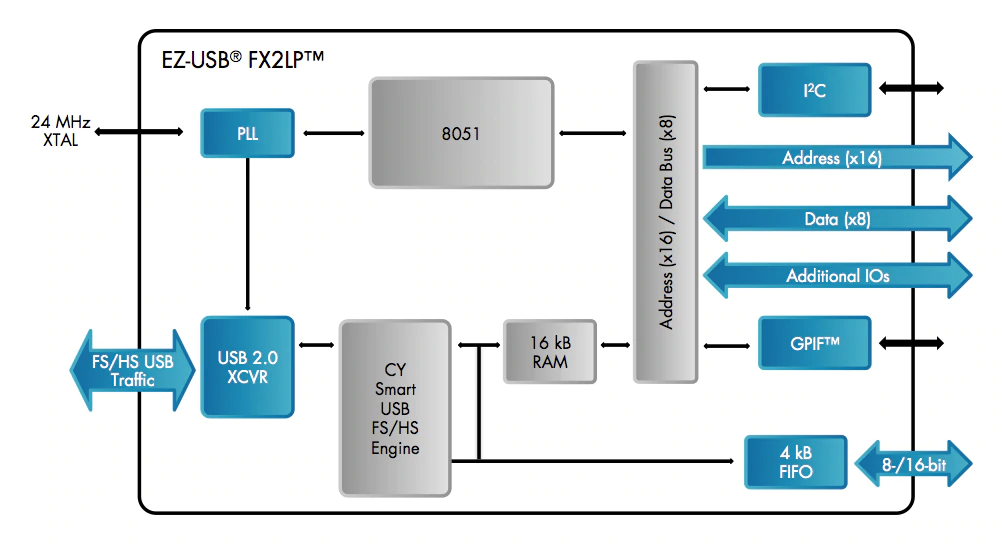
\includegraphics[width=\textwidth]{fx2lp}
		\end{column}
		\begin{column}{.6\textwidth}
			\begin{itemize}
				\item Pros
				\begin{itemize}
					\item Comunicación paralela de 16 bits
					\item Microcontrolador 8051
				\end{itemize}
				\item Contras
				\begin{itemize}
					\item Requiere esfuerzo en la configuración y software dedicado
				\end{itemize}
			\end{itemize}
		\end{column}
	\end{columns}
		
	FTDI FT4222H
	\begin{columns}
		\begin{column}{.4\textwidth}
			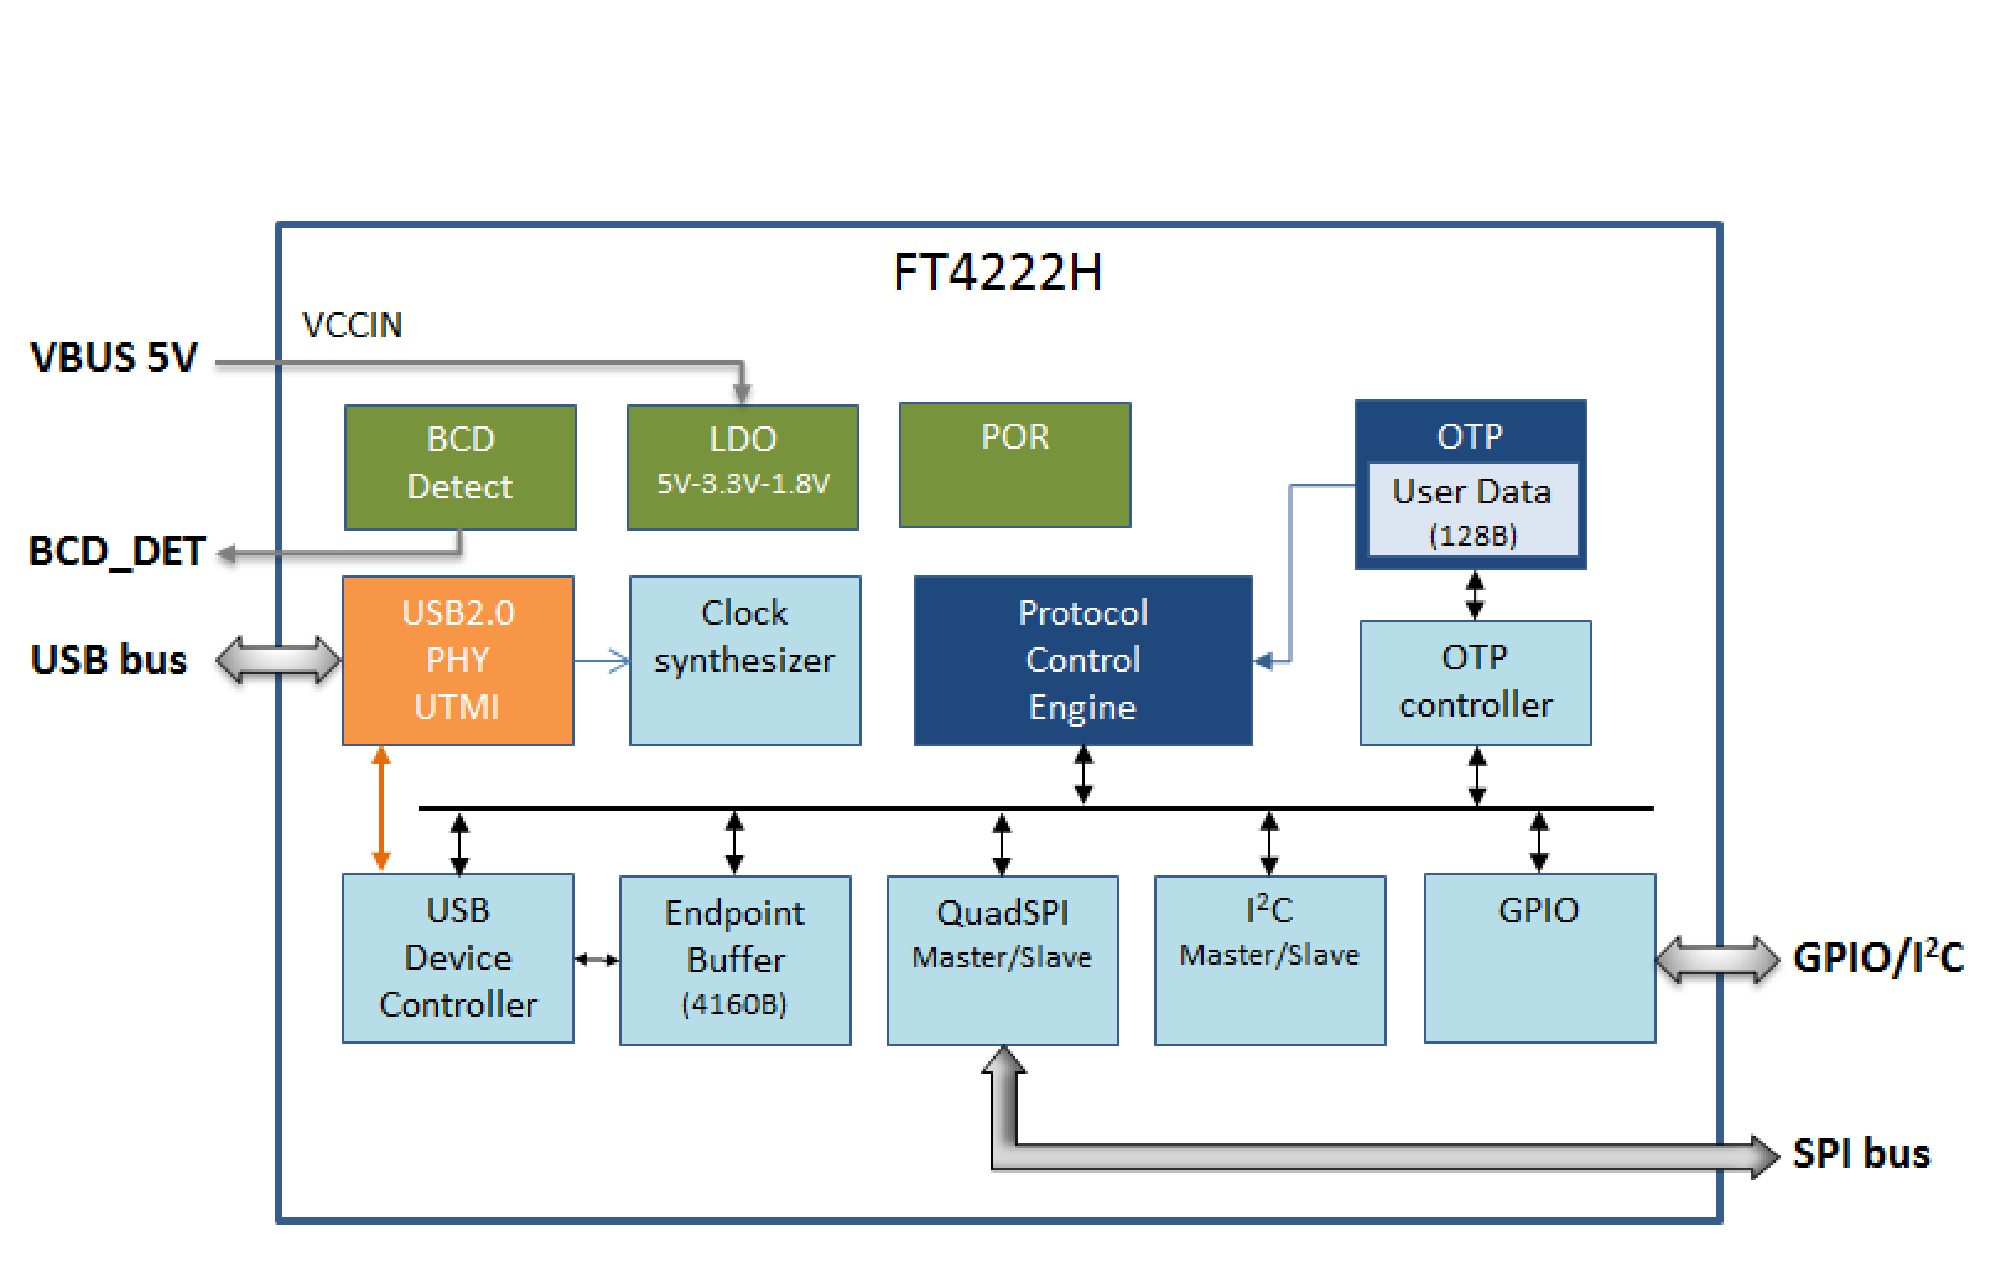
\includegraphics[width=\textwidth]{ft4222h}
		\end{column}
		\begin{column}{.6\textwidth}
			\begin{itemize}
				\item Pros
				\begin{itemize}
					\item No requiere programación
					\item Económico
				\end{itemize}
				\item Contras
				\begin{itemize}
					\item Solo permite Transferencias en Masa
					\item Comunicación SPI cuádruple
				\end{itemize}
			\end{itemize}
		\end{column}
	\end{columns}

\end{frame}

\begin{frame}{Selección del FPGA}
	\begin{columns}
		\begin{column}{.28\textwidth}
			\centering
			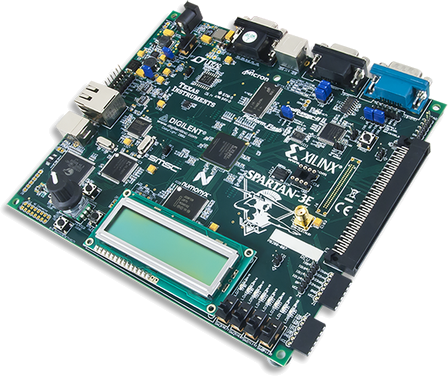
\includegraphics[width=\textwidth]{s3eboard}\\
			\centering
			Spartan-3E Starter\\
			\begin{itemize}
				\item FPGA Spartan 3E de Xilinx
				\item Gran cantidad de periféricos
			\end{itemize}
		\end{column}
		\begin{column}{.28\textwidth}
			\centering
			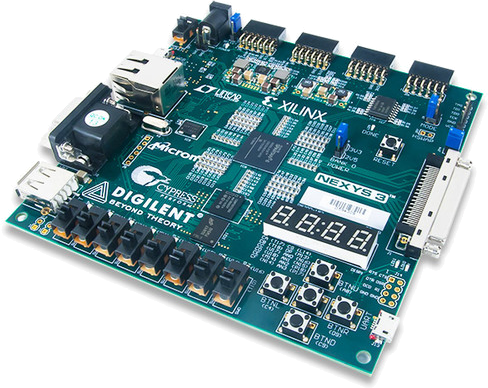
\includegraphics[width=\textwidth]{nexys3}\\
			\centering
			Nexys 3\\
			\begin{itemize}
				\item FPGA Spartan 6 de Xilinx
				\item Gran cantidad de periféricos
			\end{itemize}
		\end{column}
		\begin{column}{.28\textwidth}
			\centering
			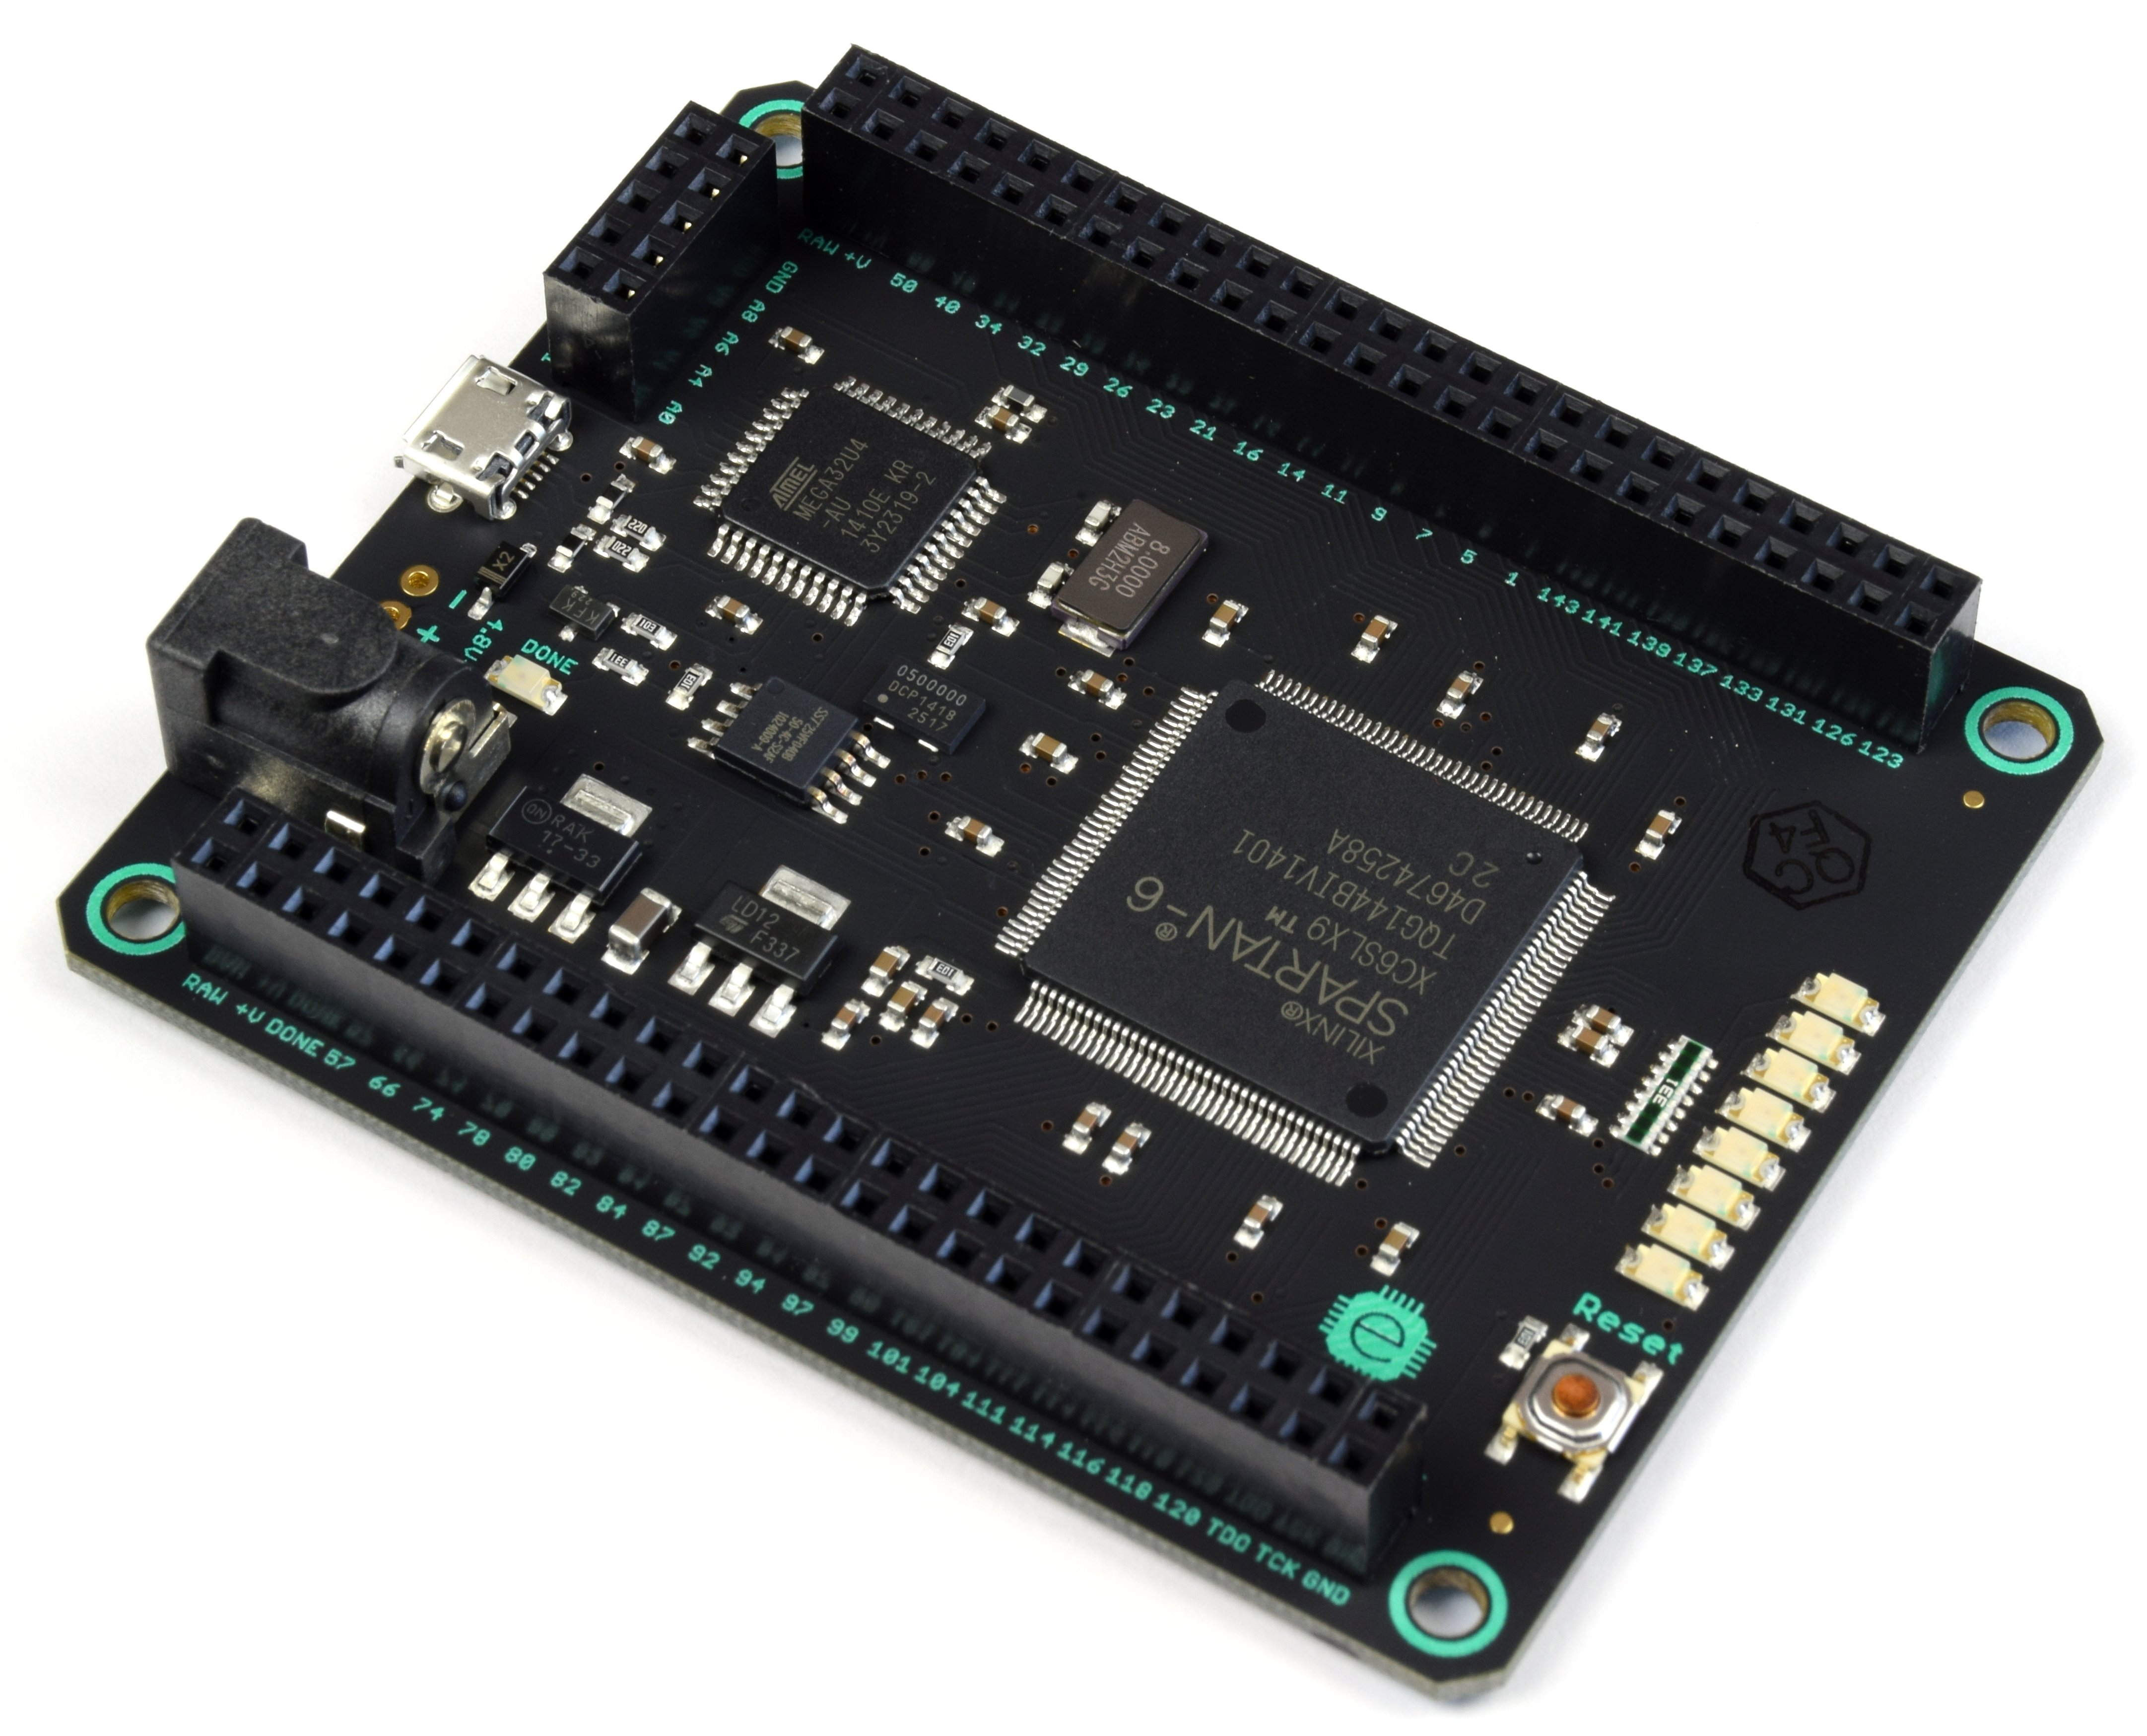
\includegraphics[width=\textwidth]{MojoIso}\\
			\centering
			\alert<2>{Movo v3\\}
			\begin{itemize}
				\item FPGA Spartan 6 de Xilinx
				\item Muy económica
			\end{itemize}
		\end{column}
	\end{columns}
\end{frame}

\begin{frame}{La placa de desarrollo MOJO v3}
	\begin{columns}
		\begin{column}{.43\textwidth}
			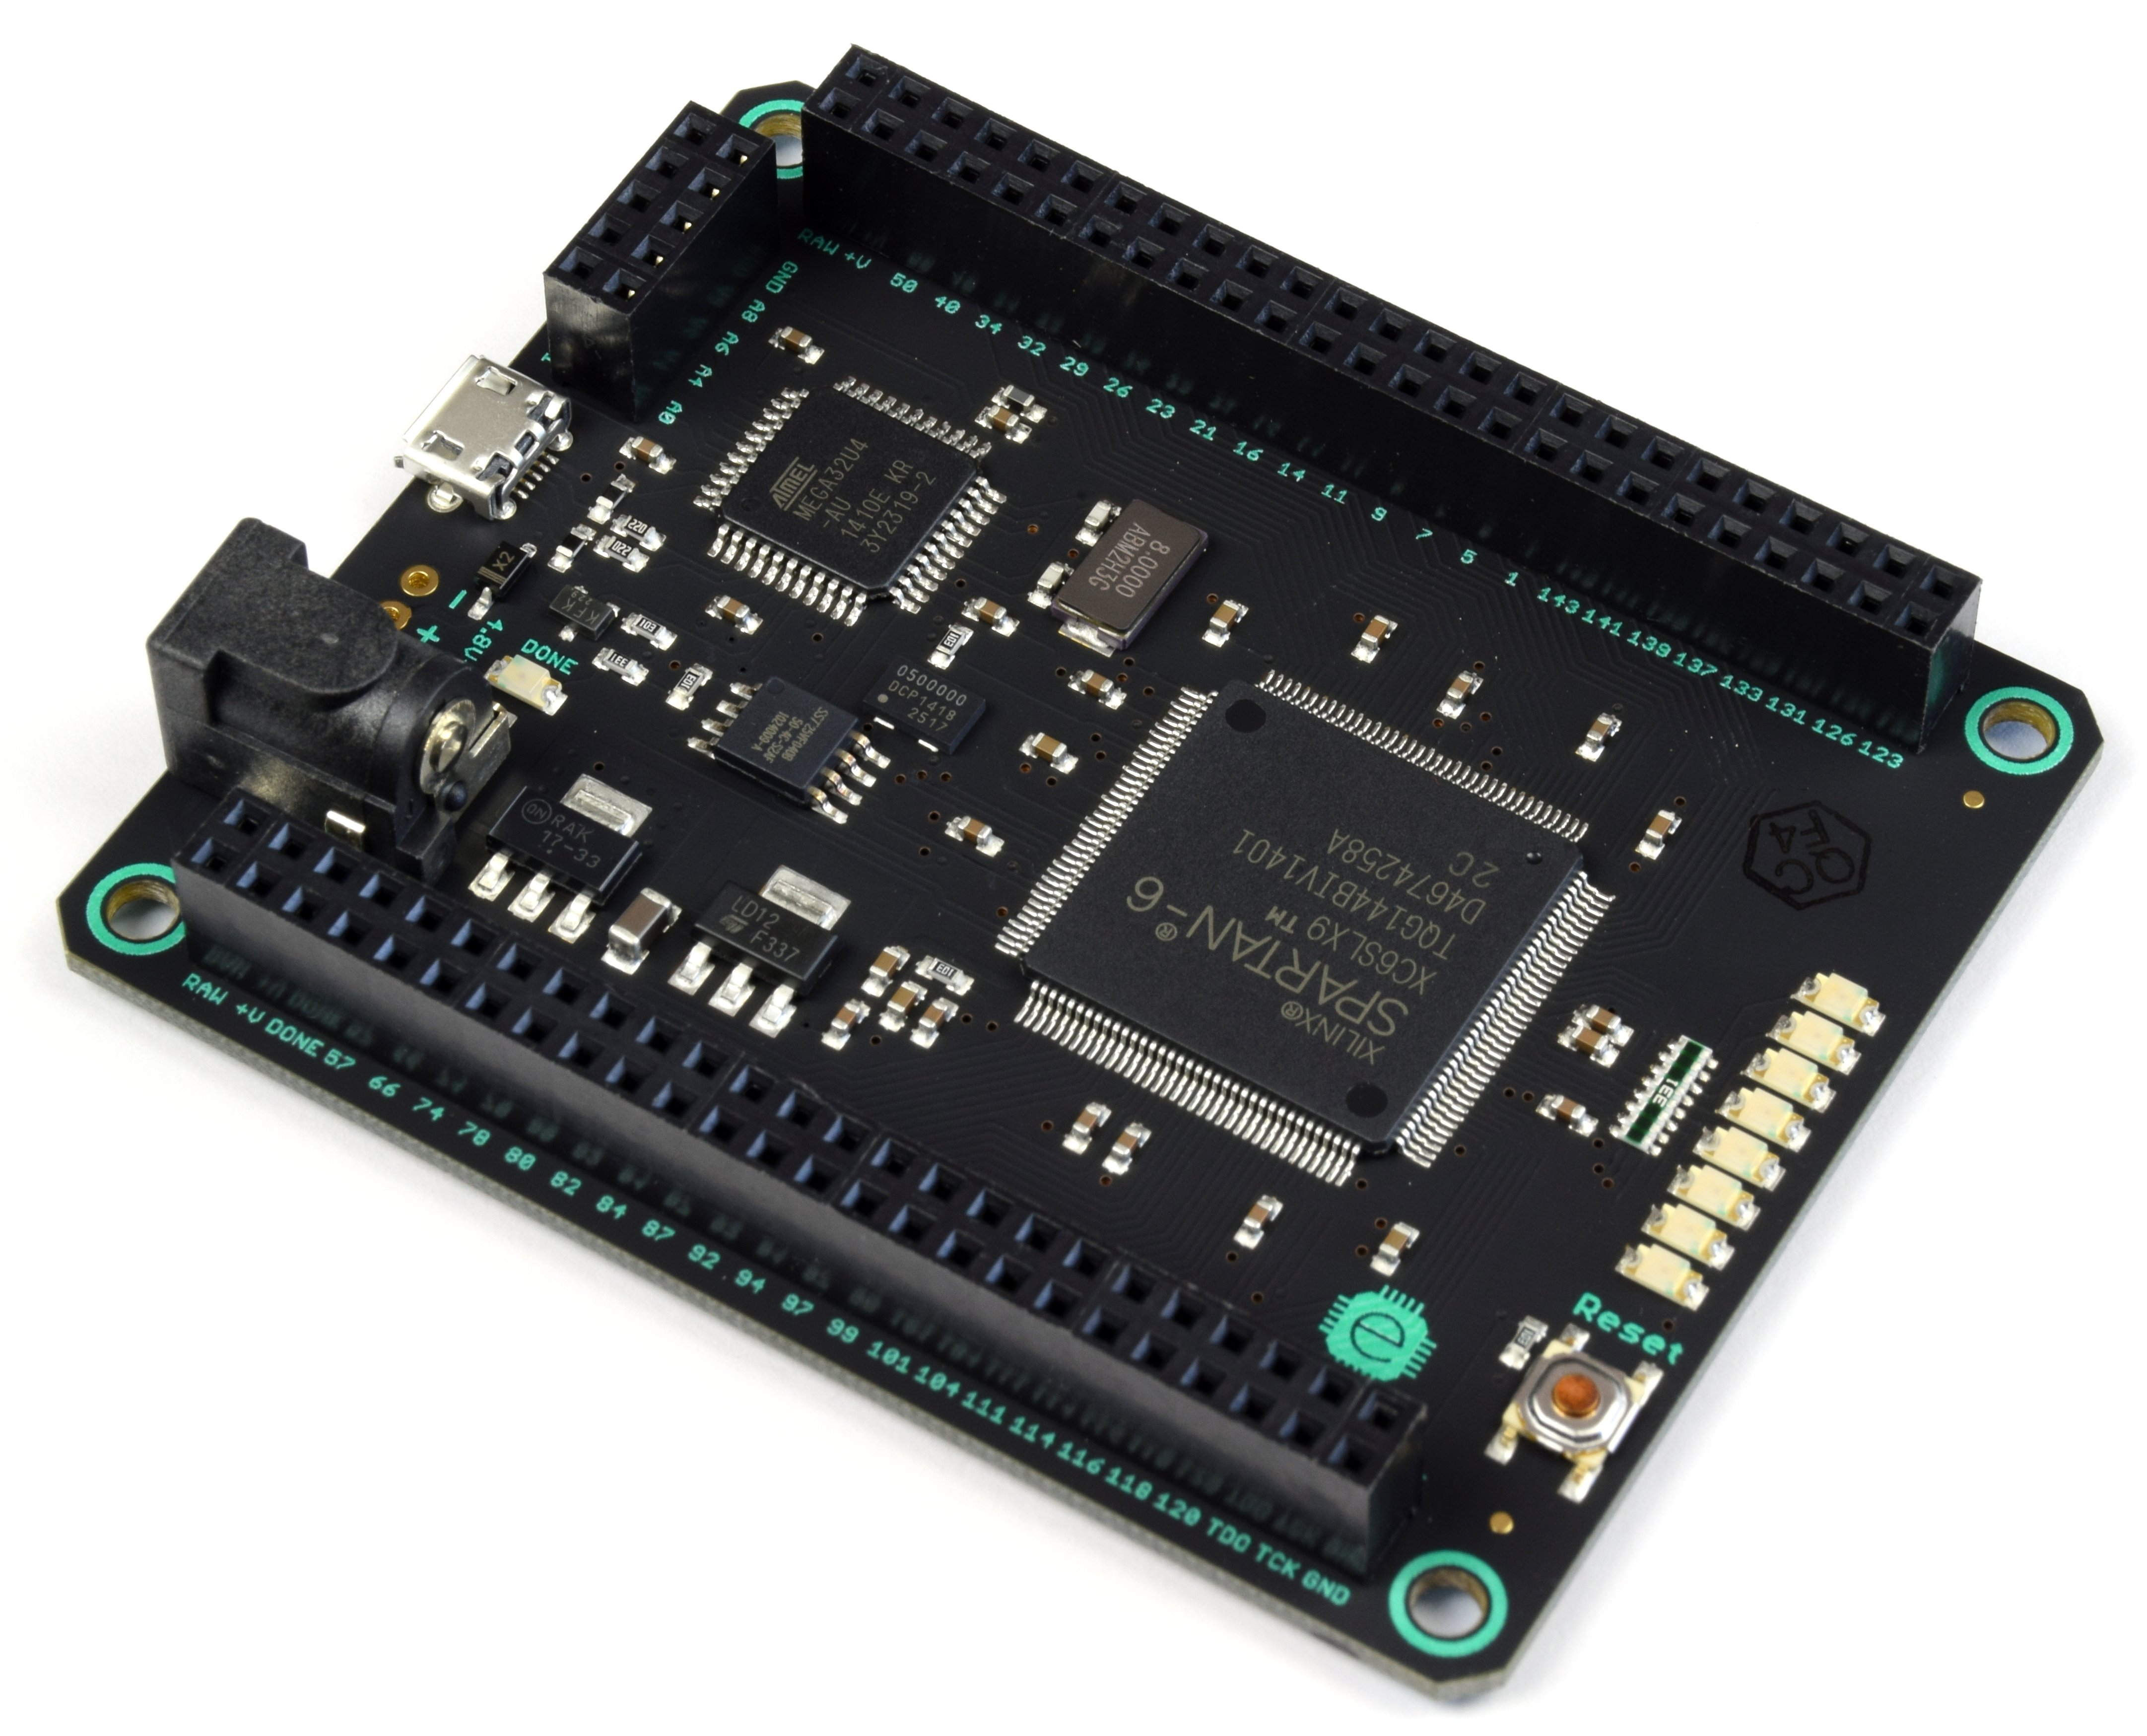
\includegraphics[width=\textwidth]{MojoIso.png}
		\end{column}
		\begin{column}{.55\textwidth}
			\begin{itemize}
				\only<1>{
					\item FPGA Spartan 6 XC6SLX9 de Xilinx
					\item 84 pines IO digitales
					\item 8 entradas analógicas
					\item 8 LEDs de propósito general
					\item 1 pulsador de propósito general
					\item ATmega32U4 para configurar la FPGA y leer los pines analógicos.
					\item Memoria flash para almacenar la configuración de la FPGA.}
				\item USB para programación y comunicación.
				\only<2>{
					\begin{itemize}
						\item USB 2.0 Full-Speed de 12 Mbps
						\item Implementado a través de controlador ATmega32U4
						\item Interfaz FPGA-ATmega32U4 via SPI de 8 Mbps.
					\end{itemize}
				}
			\end{itemize}
		\end{column}
	\end{columns}
\end{frame}

\begin{frame}{Circuito de interconexión}
	\only<1>{
		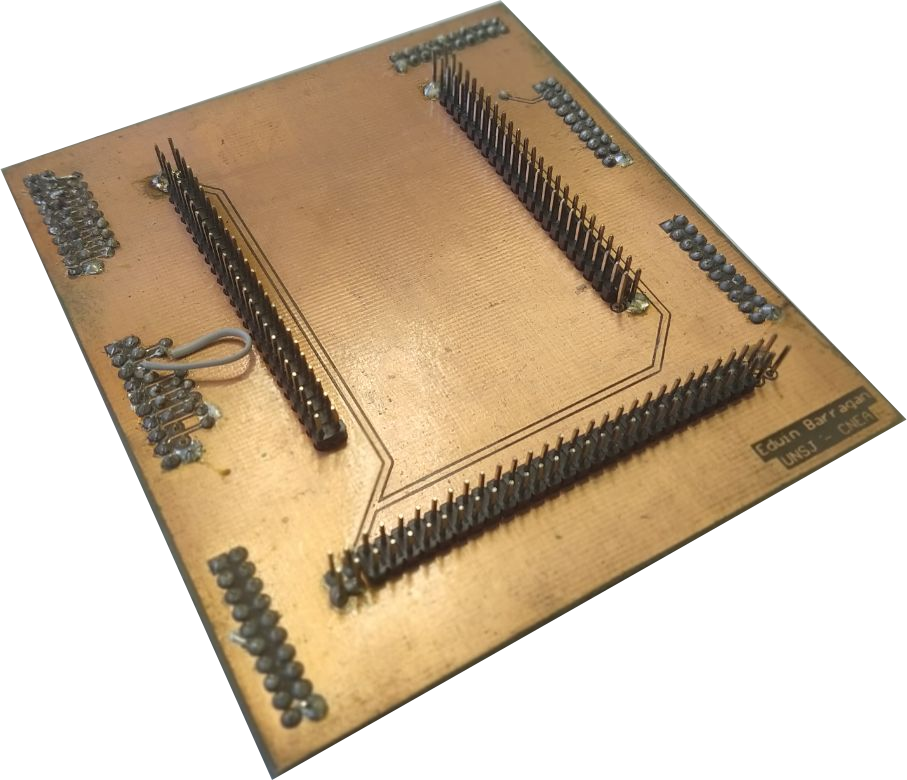
\includegraphics[width=.45\textwidth]{63v2anverso}
		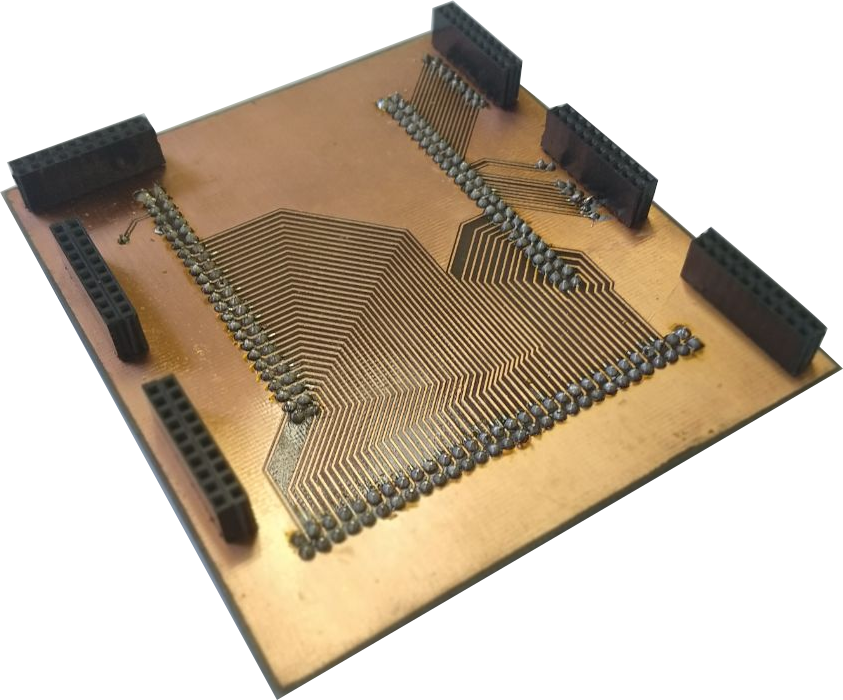
\includegraphics[width=.45\textwidth]{64v2reverso}
	}
	\only<2>{
		\centering
		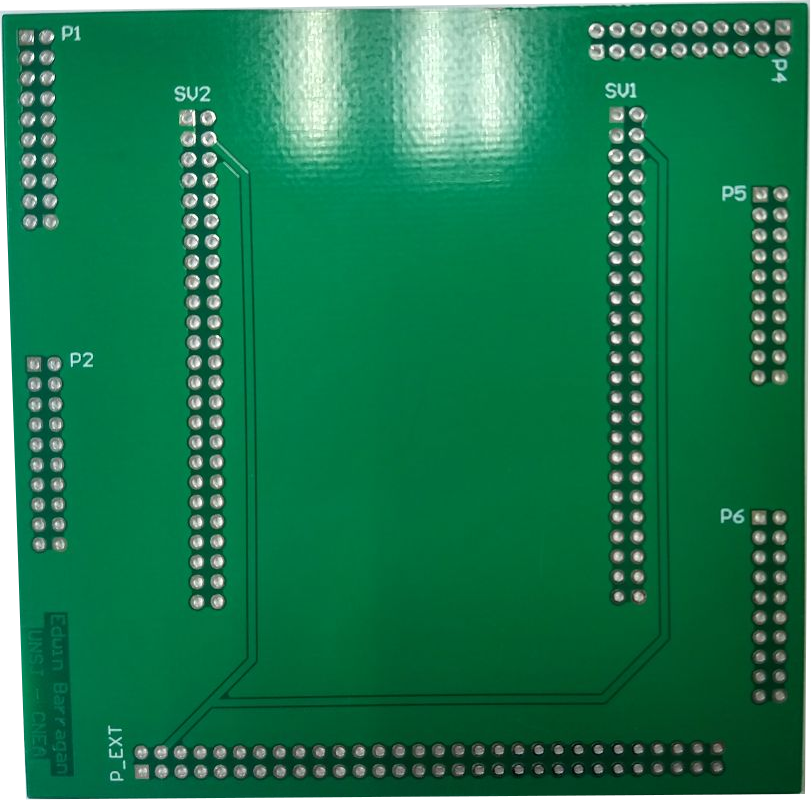
\includegraphics[width=.45\textwidth]{65v3anverso}
		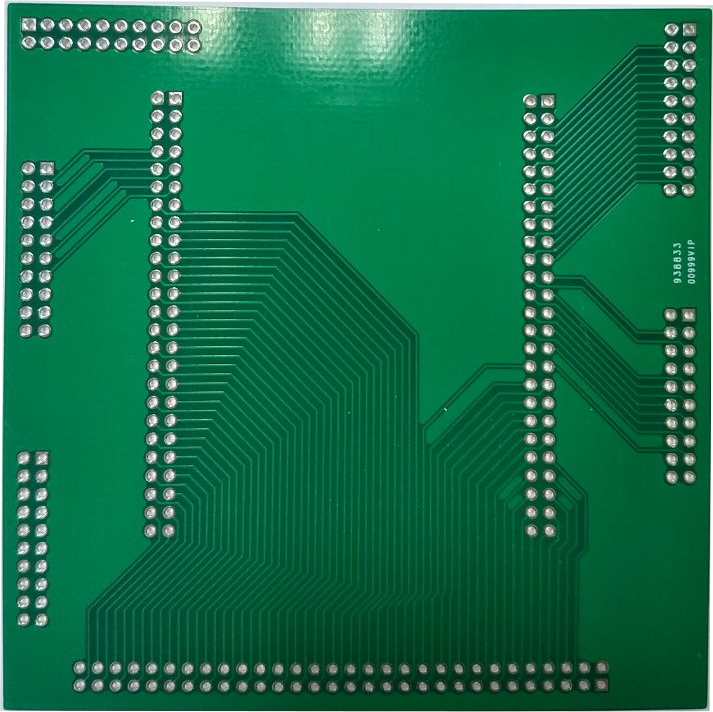
\includegraphics[width=.45\textwidth]{66v3reverso}
	}
\end{frame}

\begin{frame}{Acceso al dispositivo desde la PC}
	Para acceder al puerto USB desde la PC se utilizó la biblioteca libusb-1.0:
	\begin{itemize}
		\item Software libre: Puede ser utilizado sin necesidad de comprar una licencia.
		\item API portable: Permite escribir código que puede ser compilado en múltiples Sistemas Operativos.
		\item Abundante documentación: Se encuentran en Internet manuales y tutoriales muy completos sobre su funcionamiento.
	\end{itemize}
\end{frame}

\begin{frame}{Componentes del sistema}
	\begin{tikzpicture}[scale=1,>=latex]
	\begin{scope}
	\begin{scope}[transform shape,node distance=2]
	\node[bloque]	(cy)				{Interfaz\\\alert{Cypress FX2LP}};
	\node[bloque]	(fpga)	[right=of cy]{FPGA\\\alert{Xilinx Spartan VI}};
	\node[bloque]	(pc) 	[left=of cy]	{PC\\\alert{libusb}};
	\draw[->,thick] (pc.15) -- node (usbd+) [above]	{D+} (pc.15 -| cy.west);
	\draw[->,thick] (cy.195) -- node (usbd-) [below]	{D-} (cy.195 -| pc.east);
	\draw[<->,thick] (cy.15) -- node (data) [above] {Datos} (cy.15 -| fpga.west);
	\draw[->,thick]  (fpga.195) -- node (ctrl) [below] {Control} (fpga.195 -| cy.east);
	\node[node distance=.4,text=blue] (usb text) [above=of usbd+] {USB};
	\node[node distance=.5,text width=60,align=center,text=blue] (pcb text)[above=of data]{Placa de\\Interconexión};
	\end{scope}
	\begin{scope}
	\node[rectangle,rounded corners,draw=blue,dashed,fit=(usb text)(usbd+)(usbd-)(cy.south west)(pc.east)](usb){};
	\node[rectangle,rounded corners,draw=blue,dashed,fit=(cy.south east)(fpga.north west)(pcb text)](pcb){};
	\end{scope}
	\end{scope}
	\end{tikzpicture}
\end{frame}

\begin{frame}{Sistema completo}
	\centering
	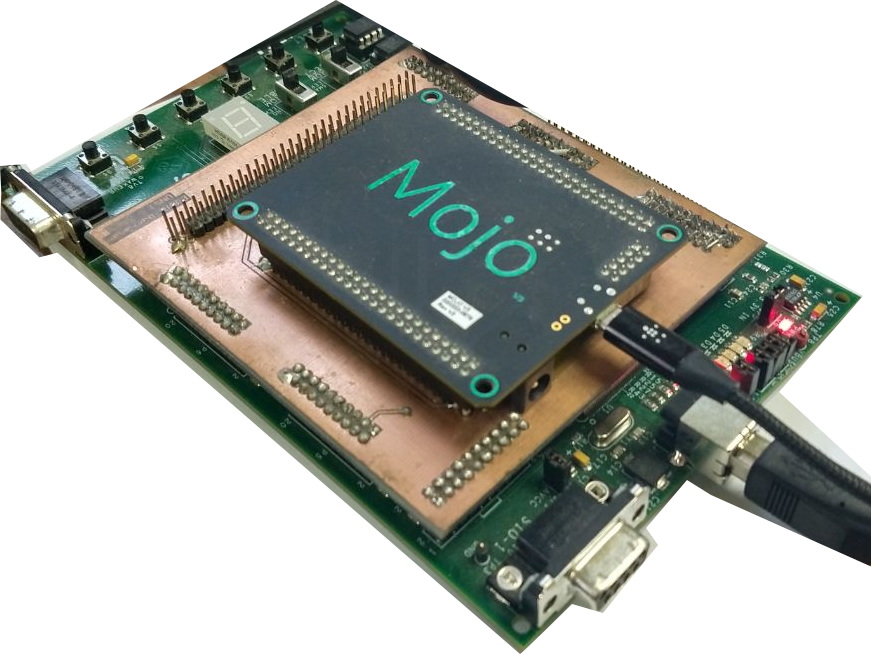
\includegraphics[width=.6\textwidth]{fisico}
\end{frame}

		\subsection{Configuración de la Interfaz USB}
			%La comunicación entre la PC y el FPGA se realiza mediante tres bloques, los que se pueden apreciar en la Figura \ref{fig:etp}: la comunicación entre el FPGA y la interfaz, la configuración de la interfaz misma y la conexión entre la PC y la interfaz. El desarrollo de cada etapa cuenta con herramientas específicas que facilitan en gran medida la tarea que se realiza. En este capítulo se detalla por separado las características de cada una de estas herramientas.
%Se puede descomponer la implementación en tres partes bien definidas: La comunicación entre el FPGA y la interfaz intermedia, la configuración de la interfaz misma, y la conexión entre la PC y la interfaz. El desarrollo de cada una de estas etapas contará con herramientas específicas.\\

%\begin{figure}
%	\centering
%	\begin{tikzpicture}[]
%	\begin{scope}[transform shape,node distance=1,>=latex]
%	\node[rectangle, rounded corners,draw=black,minimum size=40](memo){Memoria};
%	\node[](aux01)[right=of memo]{};
%	\node[align=center,](comFIFO)[above=of aux01]{Comunicacion\\Interfaz - FPGA};
%	\node[exterior](fpga)[right=of aux01]{FPGA};
%	\node[rectangle, rounded corners, draw=black, minimum size=40,align=center](trans)[left=of memo]{Transceptor\\USB};
%	\node[node distance=.5](aux02)[left=of memo]{};
%	\node[](interfaz)[below=of aux02]{Interfaz};
%	\node[](aux03)[left=of trans]{};
%	\node[align=center](comPC)[above=of aux03]{Comunicación\\PC - Interfaz};
%	\node[exterior](pc)[left=of aux03]{PC};
%	\draw[thick,<->] (fpga) to (memo);
%	\draw[thick,<->] (pc) to (trans);
%	\end{scope}
%	\begin{scope}[]
%	\node[rectangle, dashed, draw=black, rounded corners, fit={(fpga)(memo)(comFIFO)}] (parte1) {};
%	\node[exterior,fit={(trans)(interfaz)(memo)}](bridge){};
%	\node[rectangle, rounded corners, dashed,draw=black, fit={(trans)(pc)(comPC)}](parte3){};
%	\node[rectangle, rounded corners, dashed,draw=black, fit={(interfaz)(bridge)}](){};
%	\end{scope}
%	\end{tikzpicture}
%	\caption{Partes en que se desglosa el trabajo}
%	\label{fig:etp}
%\end{figure}


La parte central del sistema desarrollado en el presente trabajo está constituida por el módulo de interfaz entre el FPGA y la PC. La función de este módulo es comunicarse con una PC a través del protocolo USB 2.0, decodificando los paquetes que recibe la interfaz FX2LP, comprobando que dichos paquetes no contengan errores, separando la información del protocolo USB (encabezado y cola), de la que es útil para el sistema implementado en un FPGA. Además, debe escribir los datos recibidos desde la PC en el FPGA con un protocolo más simple, con el objetivo de utilizar menos recursos programables de este último dispositivo. También debe efectuar el camino inverso de comunicación, es decir leer datos del FPGA, colocar la información que requiere el protocolo y transmitir los paquetes hacia la PC.%\\

En el mercado de componentes electrónicos, existen dos fabricantes que ofrecen interfaces USB (también llamadas puentes USB). Las empresas FTDI y Cypress Semiconductor exhiben en sus catálogos, sendas líneas de productos que proveen circuitos integrados que podrían servir a los fines del desarrollo buscado. Durante la elaboración de este trabajo, se evaluó la alternativa que más se ajusta a las necesidades del sistema desarrollado que brinda cada uno de estos proveedores.

El chip FT4222H de FTDI es un puente USB relativamente simple de configurar, ya que no es necesario elaborar software adicional para que ejecute las tareas relativas a la comunicación. Hacia el lado de los periféricos, la comunicación se realiza mediante el protocolo SPI, con un reloj de hasta \SI{30}{\mega\hertz}. Es posible alcanzar la velocidad máxima permitida por el protocolo USB mediante el uso de cuatro puertos SPI.%Sin embargo, posee una desventaja importante con respecto a los objetivos del presente trabajo. La interfaz de FTDI se comunica con los periféricos que necesitan enviar datos a través de él por un puerto SPI, cuya tasa máxima de transferencia de \SI{53.8}{\mega\bit\per\second}~\cite{FutureTechnologyDevicesInternationalLtd}. Esta característica hace que no sea apropiada para el sistema que se desarrolla.

Por su parte, la línea de circuitos integrados FX2/FX2LP de Cypress Semiconductor ofrece controladores USB muy versátiles y potentes. Los puentes USB poseen, cómo interfaz hacia los periféricos, un conjunto de memorias FIFO a las que se puede acceder por un puerto paralelo de 16 bits de ancho de bus, que pueden operar a 48 MHz. También incorporan un microcontrolador 8051, el cual implementa niveles superiores del protocolo USB, ejecutando las tareas de configuración y control que solicita el Host \cite{CypressSemiconductor2014fx2lp}, y a su vez, puede ser utilizado por el usuario para implementar sistemas adicionales.

Se escoge entonces, para el desarrollo del sistema de comunicación, el controlador FX2/FX2LP de Cypress en lugar de la interfaz fabricada por FTDI ya que el uso de un puerto cuádruple SPI supone una implementación un poco más costosa, en términos de lógica programable, que la comunicación de un puerto paralelo de 16 bits.

Cypress comercializa un kit de desarrollo destinado al diseño de sistemas basados en la serie de controladores FX2LP. Dicho kit de desarrollo se denomina CY3684 EZ-USB FX2LP. El kit posee una placa de desarrollo como la que se observa en la Figura \ref{fig:cy3684}. El componente principal del kit es el controlador EZ-USB FX2LP e incorpora un display de 7 segmentos, 4 luces led multipropósito, 6 pulsadores, de los cuales 4 son de propósito general, uno de reinicio y otro que envía una señal especial para salir de un modo de bajo consumo. También tiene dos memorias EEPROM destinadas al almacenamiento del firmware (programa que ejecuta un microcontrolador), posibilitando la carga no volátil de la configuración del controlador; una memoria Flash con una capacidad de \SI{64}{\kilo\byte} que es utilizada durante la ejecución del firmware, un puerto USB y dos UART con conectores DE-9. Adicionalmente, cuenta con 6 puertos de 20 pines, compatibles con Analizadores Lógicos estándar y un puerto con 40 pines, compatible con el protocolo ATA, que permiten comunicarse con el controlador.
 
%El controlador EZ-USB FX2LP fabricado por Cypress Semiconductor, un circuito integrado que posee en su interior una versión del microcontrolador ($\mu$C) Intel 8051, con algunas mejoras destinadas a satisfacer mejor los requerimientos del sistema USB; una interfaz que permite ingresar datos en serie y los entrega en forma paralela y viceversa; un transceptor USB encargado de todas las tareas de codificación y decodificación de paquetes USB; memoria RAM para programas y datos de \SI{16}{\kilo\byte}. Posee, a su vez, tres tipos de interfaces hacia periféricos externos: I$^2$C, una memoria FIFO (Primero Entrado, Primero Salido, del inglés{\it First In First Out}) destinada a sistemas que pueden comandar la lectura y escritura de datos, y un sistema de propósito general que puede ser comandado a través del $\mu$C 8051~\cite{CypressSemiconductor2014fx2lp}.%\\%a través del cual efectua las tareas que requiere la comunicación USB, sumado a un transceptor USB, el cual codifica y decodifica los paquetes USB que se transmiten a través del bus. A su vez, posee ciertos periféricos e interfaces que otorgan flexibilidad suficiente para adecuar el chip a los requerimientos de un desarrollo determinado.\\

%El controlador viene montado en un circuito impreso que posee una serie de componentes adicionales que facilitan la interacción del desarrollador, tales como pulsadores, display de 7 segmentos, módulos de memoria adicional,etc. Este tipo de circuitos impresos armados con la intención de favorecer desarrollo de otros sistemas, se denomina placa de desarrollo. Una placa de desarrollo que, además, incorpora algunas herramientas extra como software, cables de conexión, fuentes, etc. toma el nombre de kit de desarrollo.%\\

\begin{figure}[ht]
\centering
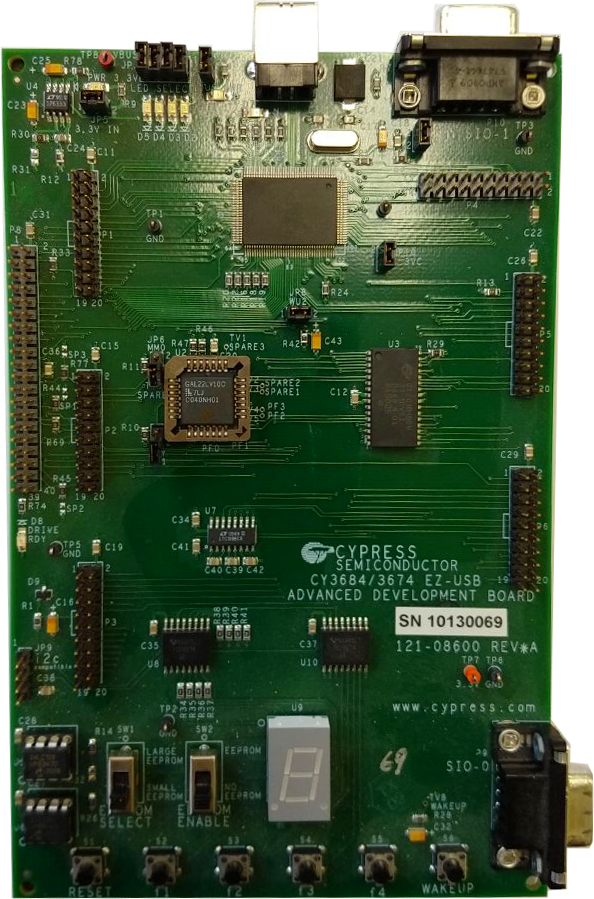
\includegraphics[width=0.4\textwidth]{32cypressboard}
\caption{Circuito impreso principal del kit de desarrollo CY3684 EZ-USB FX2LP}
\label{fig:cy3684}
\end{figure}

%En este trabajo, se utiliza el kit de desarrollo CY 3684 EZ-USB FX2LP, fabricado por Cypress Semiconductor~\cite{CypressSemiconductor2014cy3684}. El kit posee una placa de desarrollo como la que se observa en la Figura \ref{fig:cy3684}. El componente principal del kit es el controlador EZ-USB FX2LP e incorpora un display de 7 segmentos, 4 luces led multipropósito, 6 pulsadores, de los cuales 4 son de propósito general, uno de reinicio y otro que envía una señal especial para salir de un modo de bajo consumo. También tiene dos bloques de memorias EEPROM destinadas al almacenamiento del firmware (programa que ejecuta un microcontrolador), lo que otorga la posibilidad de realizar una carga no volátil de la configuración del controlador, memoria flash de \SI{64}{\kilo\byte} utilizados como RAM por el programa del controlador, un puerto USB y dos puertos UART con zócalos DE-9. Adicionalmente, cuenta con 6 puertos de 20 pines que permiten comunicarse con el controlador y 1 puerto de 40 pines, compatible con el protocolo ATA.%\\
%AQUI QUEDE

%	La arquitectura del controlador EZ-USB FX2LP se muestra en la Figura %TODO la arquitectura, pavo
%	. En ella se puede apreciar los diferentes componentes que se integran en él. Como se menciona anteriormente, la serie de circuitos integrados EZ-USB FX2LP incorporan un microcontrolador 8051, con algunas mejoras destinadas a satisfacer mejor los requerimientos del sistema USB; una interfaz serie, que permite ingresar datos uno tras otro y los entrega en forma paralela y viceversa; un transceptor USB encargado de todas las tareas de codificación y decodificación de paquetes USB; memoria RAM para programas y datos de \SI{16}{\kilo\byte}. Posee, a su vez, tres tipos de interfaces hacia periféricos externos


%	Como interfaz entre la FPGA y la PC se utilizó kit de de desarrollo CY3684 FX2LP EZ-USB Development Kit de Cypress Semiconductor,la que se observa en la Figura \ref{cy3684}. Esta placa posee como núcleo el controlador USB CY7C68013A, circuito integrado que posee todas las herramientas necesarias para realizar la interfaz, como así también un buen número de periféricos que permiten al desarrollador realizar pruebas y depuración.\\


%	Entre estas, se destacan 6 pulsadores, de los cuales cuatro se utilizan para proposito general, uno para reestablecer los valores por defecto de la placa y uno para enviar señales de suspensión y reestablecimiento del programa actualmente cargado en el microcontrolador, lo que coloca al sistema en modo bajo consumo de energía. A su vez, posee dos memorias EEPROM que sirven para cargar firmware y archivos de configuración del sistema, un display de 8 segmentos, 4 leds de multiple propósito, dos puertos UART, una salida de pines compatible con puertos ATA y 6 puertos de 20 pines que se utilizan para la conexión hacia el chip núcleo. Como soporte para el firmware, posee también un bloque con \SI{64}{\kilo\byte} de memoria SRAM.\\

%Se selecciona este controlador como interfaz ya que cuenta con una gran cantidad de herramientas que permiten realizar la comunicación USB, además de poseer memoria suficiente para datos y una interfaz de comunicación para periféricos simple lo que facilita el objetivo de utilizar la menor cantidad de los recursos configurables del FPGA, de forma tal que queden, estos últimos, disponibles para el desarrollo de otros sistemas.%\\

		\subsection{Desarrollo de la Máquina de Estados Finitos}
			\begin{frame}{La placa de desarrollo MOJO v3}
	\begin{columns}
		\begin{column}{.43\textwidth}
			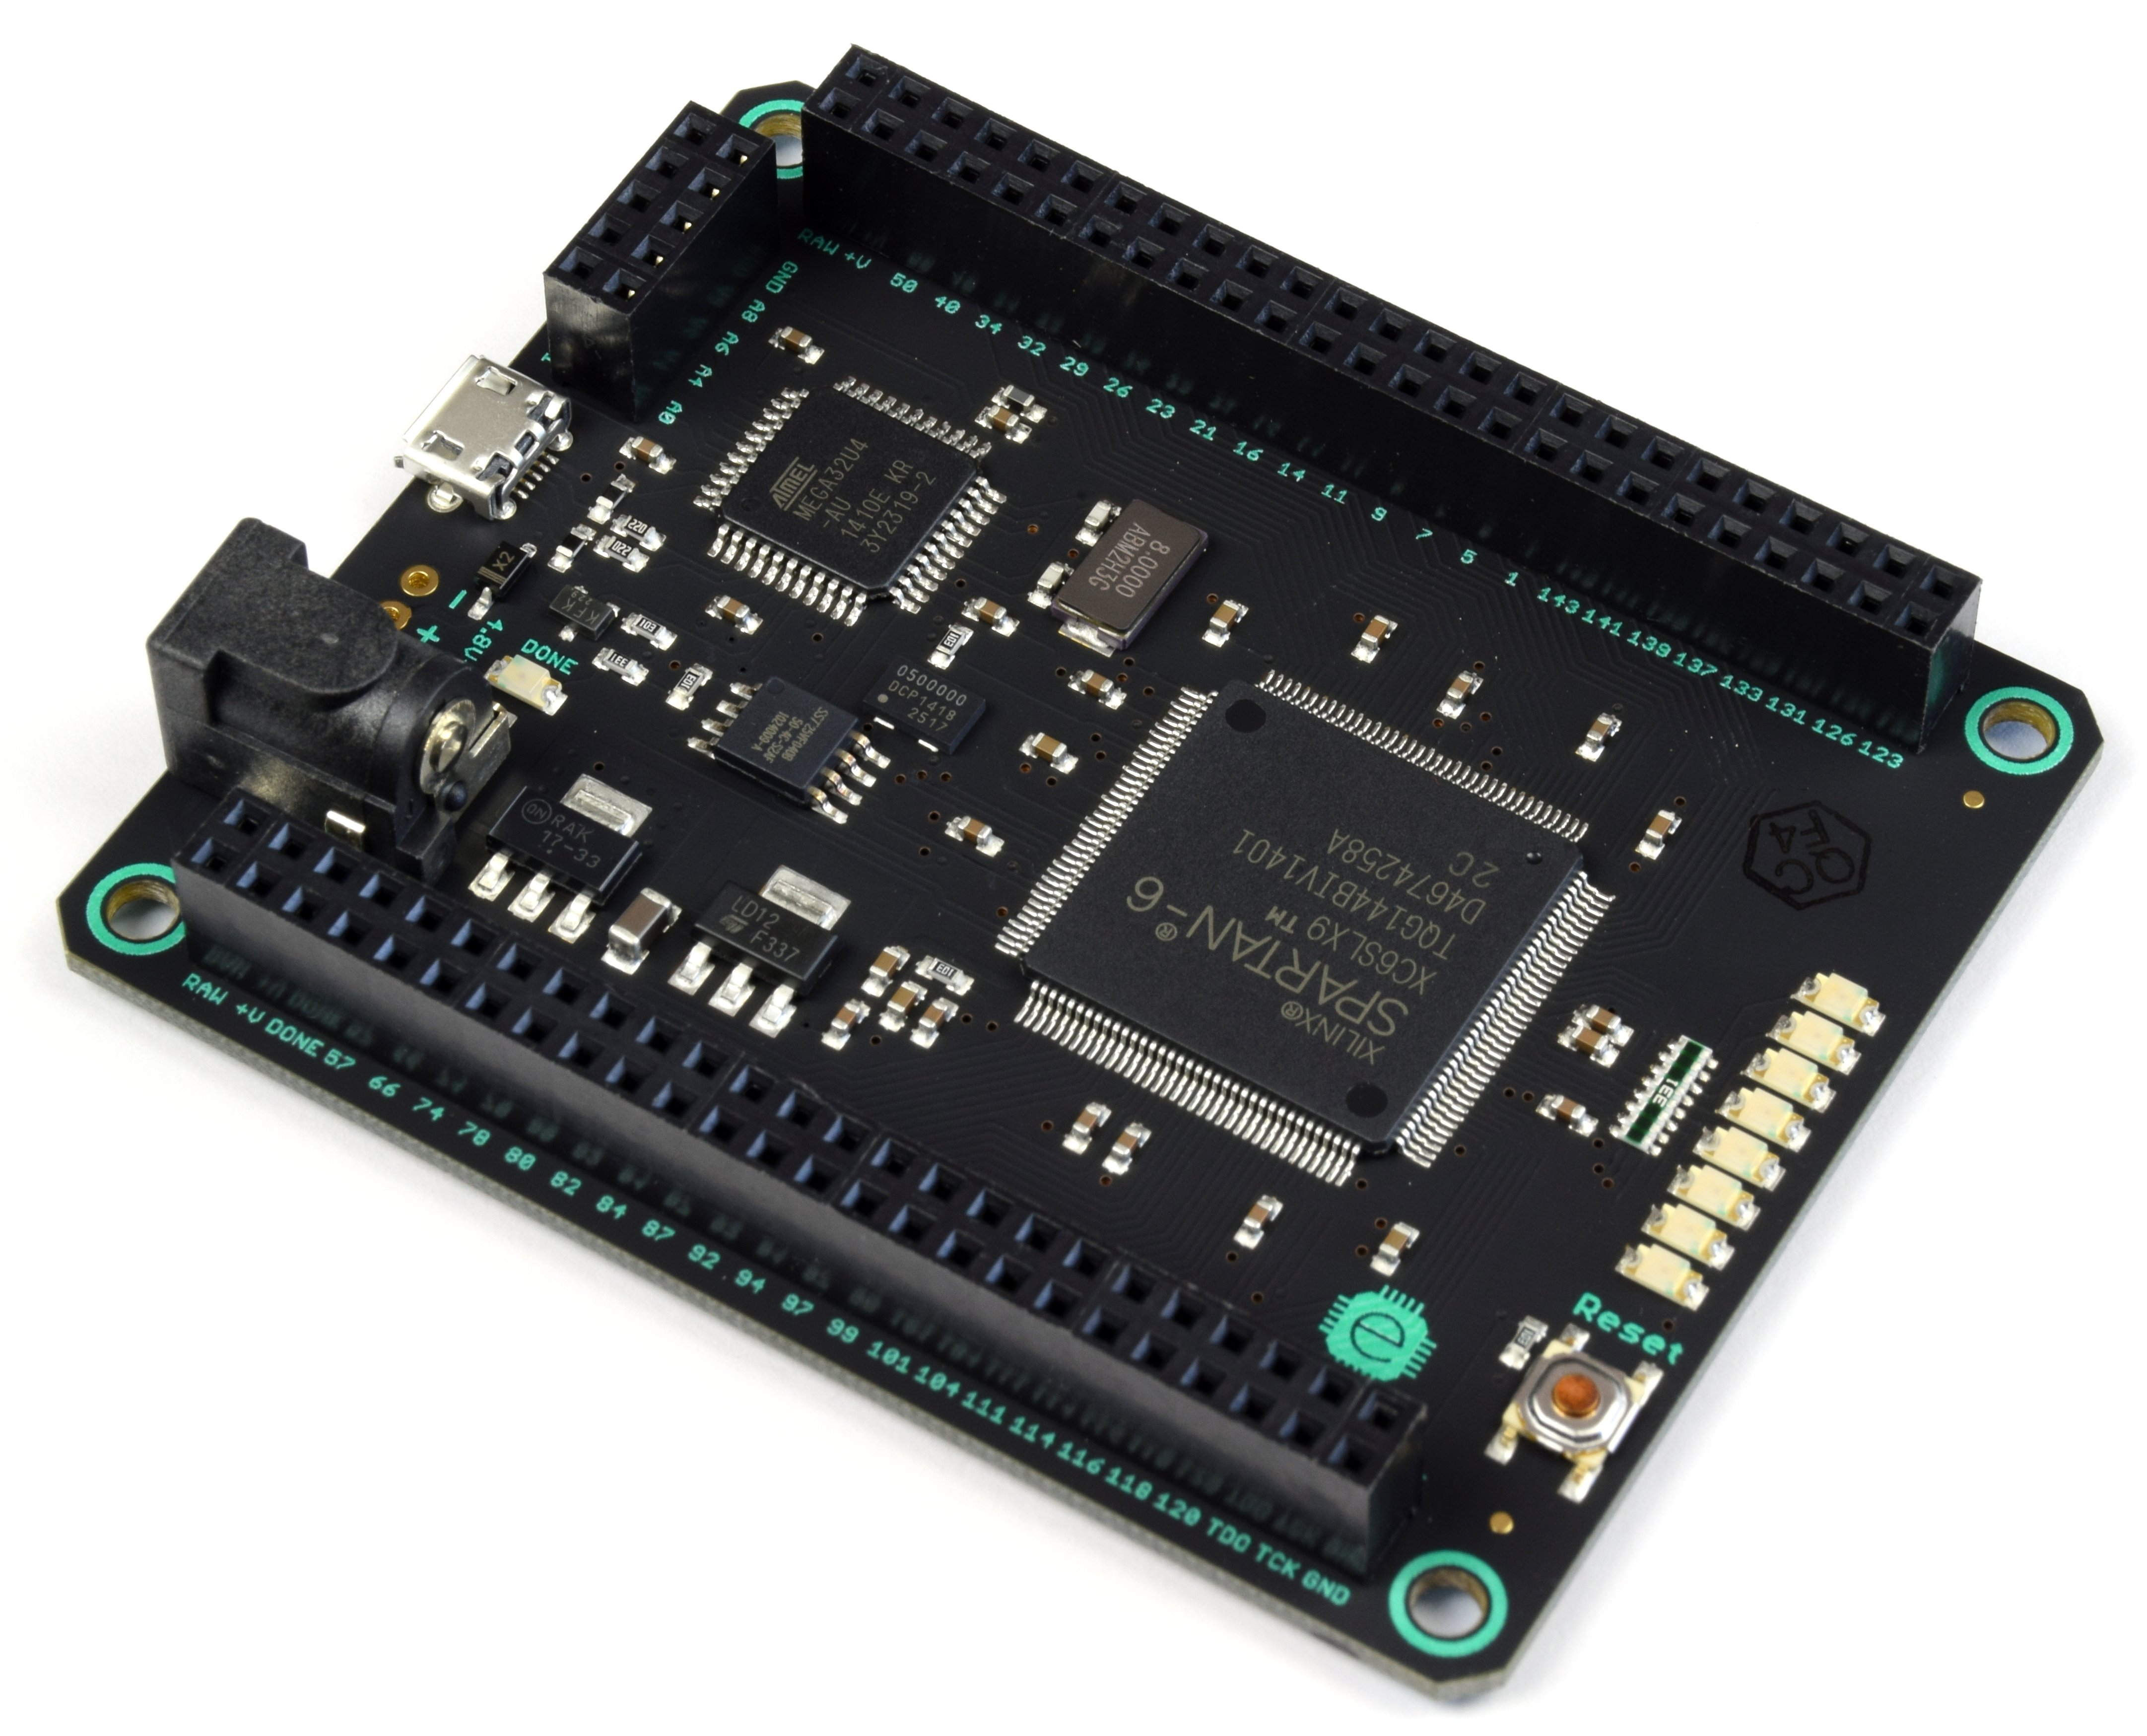
\includegraphics[width=\textwidth]{MojoIso.png}
		\end{column}
		\begin{column}{.55\textwidth}
			\begin{itemize}
				\item FPGA Spartan 6 XC6SLX9 de Xilinx
				\item 84 pines IO digitales
				\item 8 entradas analógicas
				\item 8 LEDs de propósito general
				\item 1 pulsador de propósito general
				\item Regulador de voltaje de entrada de 4.8V - 12V
				\item ATmega32U4 para configurar la FPGA y leer los pines analógicos
				\item Bootloader compatible con Arduino
				\item Memoria flash para almacenar la configuración de la FPGA (programación persistente)
			\end{itemize}
		\end{column}
	\end{columns}
\end{frame}
\begin{frame}{Estructura interna FPGA}
	\centering
	\begin{tikzpicture}[scale=.58]
		\begin{scope}[transform shape,node distance=5,>=latex,thick]
			\node[simple]	(cypress)		[]	 			{FIFO Esclava};
			\node[simple]	(master)	[right=of cypress]	{Maestro Externo};
			\node[simple,minimum size=70]	(leer)		[right=of master.north west,anchor=north west] {Leer FIFO};
			\node[simple,minimum size=70]	(escribir)	[right=of master.south west,anchor=south west]	{Escribir FIFO};
			\node[simple,node distance=8]	(fifo)		[right=of master]	{FIFO Interna (XLNX core generator)};
			
			\draw[<->]	([yshift=4*110/6]cypress.east) --node [above]{IFCLK} ([yshift=4*110/6]master.west);
			\draw[<->]	([yshift=3*110/6]cypress.east) --node [above]{FD[15:0]} ([yshift=3*110/6]master.west);
			\draw[<-]	([yshift=2*110/6]cypress.east) --node [above]{FIFOADR[1:0]} ([yshift=2*110/6]master.west);
			\draw[->]	([yshift=1*110/6]cypress.east) --node [above]{EP2\_EMPTY} ([yshift=1*110/6]master.west);
			\draw[->]	([yshift=0*110/6]cypress.east) --node [above]{EP8\_FULL} ([yshift=0*110/6]master.west);
			\draw[<-]	([yshift=-1*110/6]cypress.east) --node [above]{SLOE} ([yshift=-1*110/6]master.west);
			\draw[<-]	([yshift=-2*110/6]cypress.east) --node [above]{SLWR} ([yshift=-2*110/6]master.west);
			\draw[<-]	([yshift=-3*110/6]cypress.east) --node [above]{SLRD} ([yshift=-3*110/6]master.west);
			\draw[<-]	([yshift=-4*110/6]cypress.east) --node [above]{PKTEND} ([yshift=-4*110/6]master.west);
			
			\draw[<-] (leer) -- node[above]{SLWR} (master.east |- leer);
			\draw[<-] ([yshift=-1*80/7]leer.east) -- node[above]{EMPTY}([yshift=-1*80/7]fifo.west |- leer);
			\draw[->] ([yshift=1*80/7]leer.east) -- node[above]{RD\_EN}([yshift=1*80/7]fifo.west |- leer);
			
			\draw[<-] (escribir) -- node[above]{SLRD} (master.east |- escribir);
			\draw[<-] ([yshift=-1*80/7]escribir.east) -- node[above]{FULL}([yshift=-1*80/7]fifo.west |- escribir);
			\draw[->] ([yshift=1*80/7]escribir.east) -- node[above]{WR\_EN}([yshift=1*80/7]fifo.west |- escribir);			
			
			\draw[<-]	([yshift=1*110/6]fifo.west) --node [above]{DIN[15:0]} ([yshift=1*110/6]master.east);
			\draw[->]	([yshift=0*110/6]fifo.west) --node [above]{DOUT[15:0]} ([yshift=0*110/6]master.east);
			\draw[<-]	([yshift=-1*110/6]fifo.west) --node [above]{VALID} ([yshift=-1*110/6]master.east);
			
			\node[node distance=.4] (fpga) [above=of leer] {FPGA};
		\end{scope}
		\begin{scope}[on background layer]
			\node[rectangle,rounded corners,dashed,fit=(master)(leer)(fpga)(fifo)(escribir),draw=black]{};
		\end{scope}
	\end{tikzpicture}
\end{frame}
\begin{frame}{Interfaz - FPGA}
	\centering
	\begin{tikzpicture}[scale=.95]
		\begin{scope}[transform shape,node distance=5,>=latex]
			\node[simple]	(fifo)		[]	 			{FIFO Esclava};
			\node[simple]	(master)	[right=of fifo]	{Maestro Externo};
			\draw[<->,thick]	([yshift=5*110/6]fifo.east) --node [above]{IFCLK} ([yshift=5*110/6]master.west);
			\draw[<->,thick]	([yshift=4*110/6]fifo.east) --node [above]{FD[15:0]} ([yshift=4*110/6]master.west);
			\draw[<-,thick]	([yshift=3*110/6]fifo.east) --node [above]{FIFOADR[1:0]} ([yshift=3*110/6]master.west);
			\draw[->,thick]	([yshift=2*110/6]fifo.east) --node [above]{FLAGA} ([yshift=2*110/6]master.west);
			\draw[->,thick]	([yshift=1*110/6]fifo.east) --node [above]{FLAGB} ([yshift=1*110/6]master.west);
			\draw[->,thick]	([yshift=0*110/6]fifo.east) --node [above]{FLAGC} ([yshift=0*110/6]master.west);
			\draw[->,thick]	([yshift=-1*110/6]fifo.east) --node [above]{FLAGD} ([yshift=-1*110/6]master.west);
			\draw[<-,thick]	([yshift=-2*110/6]fifo.east) --node [above]{SLOE} ([yshift=-2*110/6]master.west);
			\draw[<-,thick]	([yshift=-3*110/6]fifo.east) --node [above]{SLWR} ([yshift=-3*110/6]master.west);
			\draw[<-,thick]	([yshift=-4*110/6]fifo.east) --node [above]{SLRD} ([yshift=-4*110/6]master.west);
			\draw[<-,thick]	([yshift=-5*110/6]fifo.east) --node [above]{PKTEND} ([yshift=-5*110/6]master.west);
		\end{scope}
	\end{tikzpicture}
\end{frame}
\begin{frame}{Máquina de estados algorítmica de la interfaz}
	\centering
	\begin{tikzpicture}[scale=.35]
		\begin{scope}[transform shape,node distance=1,>=latex]
			\node[moore]	(idle)	[]	{--idle:\\SLRD='1';\\SLOE='1';\\SLWR='1';\\FIFOADR="ZZ";};
			\node[ask]	(pr1)	[below=of idle]	{EP2\_empty='0'}
			edge[<-] (idle);
			\node[ask]	(pr2)	[right=of pr1]	{write\_req='1'};
			\node[ask]	(pr3)	[below=of pr2]	{EP8\_full='0'};
			\node[moore]	(radr)	[left=of pr1]		{--read address:\\SLRD='1';\\SLOE='1';\\SLWR='1';\\FIFOADR="00";};
			
			\draw[->](pr1) -- node [above,near start]{No}(radr);
			\draw[->](pr1) -- node [above,near start]{Si} (pr2);
			
			\node[node distance=0.8](aux1)[right=of pr2]{};
			\draw[->](pr2) -- node[left,near start]{Si}(pr3);
			\draw[->](pr2.east) |- node[above,near end]{No}(aux1.base);
			
			\node[moore]	(rnempty)	[left=of radr]	{--read no empty:\\SLRD='0';\\SLOE='0';\\SLWR='1';\\FIFOADR="00";}
			edge[<-](radr);
			\node[moore](rread)[below=of rnempty]{--read read:\\SLRD='1';\\SLOE='0';\\SLWR='1;\\FIFOADR="00";}
			edge[<-](rnempty);
			
			\node[moore](wadr)	[left=of pr3]	{--write address:\\SLRD='1';\\SLOE='1';\\SLWR='1';\\FIFOADR="11";};
			\node[node distance=.8](aux2)[right=of pr3]{};
			\draw[->](pr3) -- node[above,near start]{Si} (wadr);
			\draw[->](pr3) -- node[above,near start]{No}(aux2.base) -| (aux1.base);
			
			\node[moore](wnfull)[below=of wadr] {--write no full:\\SLRD='1';\\SLOE='1';\\SLWR='0';\\FIFOADR="11";}
			edge[<-] (wadr);
			\node[node distance=.5](aux3)[left=of wnfull]{};
			\draw[->] (wnfull) -- (aux3.base);
			\node[moore,node distance=.5](wwrite)[left=of aux3] {--write write:\\SLRD='1';\\SLOE='1';\\SLWR='1';\\FIFOADR="11";}
			edge[<-] (aux3.base);
			
			\node[ask](pr4)[below=of wwrite] {fifo\_valid='1'}
			edge[<-] (wwrite);
			\node[moore](wend)[left=of pr4] {--write end:\\SLRD='1';\\SLOE='1';\\SLWR='1';\\FIFOADR="11";};
			\node[node distance=.7] (aux4) [right=of pr4]{}; 
			\draw[->]	(pr4) -- node[above,near start]{Si} (wend);
			\draw[->](pr4) -- node[above] {No} (aux4.base);
			\draw[->](aux4.base) -- (aux3.base);
			
			\node[ask](pr5)[below=of wend] {write\_req='1'}
			edge[<-] (wend);
			\node[ask](pr6)[right=of pr5] {EP2\_empty='0'};
			\node[node distance=.8] (aux5) [left=of rread] {};
			\node[node distance=.8] (aux7) [left=of pr5] {};
			\draw[->] (rread) -- (aux5.base);
			\draw[->] (pr5)	-- node[above,near start] {No} (aux7.base);
			\draw[->] (pr5) -- node[above,near start] {Si} (pr6);
			
			\node[node distance=.8] (aux6)[below=of pr6] {};
			\draw[->] (pr6) -| node[above,near start] {Si} (wnfull);
			\draw[->] (pr6) -- node[left]{No} (aux6.base) -| (aux7.base);
			\draw[->] (aux7.base) |- (aux5.base);
			
			\node[node distance=.8] (aux8) [above=of idle] {};
			\draw[->] (aux8.base) -- (idle);
			\draw[->] (aux5.base) |- (aux8.base);
			\draw[->](aux1.base) |- (aux8.base);
			
		\end{scope}
	\end{tikzpicture}
\end{frame}
\begin{frame}{Maquinas de estado hacia la memoria FIFO interna}
	\begin{columns}
		\begin{column}{.5\textwidth}
			\centering
			\begin{tikzpicture}[scale=.53]
				\begin{scope}[transform shape,node distance=1,>=latex]
					\node[moore] (idle) {--idle:\\RE\_EN='0';};
					\node[node distance=.6](aux0)[above=of idle]{};
					\node[ask]	(pr1)	[below=of idle]{\tiny{SLWR='0'-$>$'1'}}
						edge[<-] (idle);
					\node[ask] (pr2) [below=of pr1]{\scriptsize{FIFO\_empty='1'}};
					\node[node distance=.8](aux1)[left=of pr1]{};
					\draw[->] (pr1) -- node[left] {Si} (pr2);
					\draw[->] (pr1) -- node[above,near start]{No} (aux1.base);
					\draw[->] (aux1.base) |- (aux0.base) -- (idle);
					
					\node[moore](rden)[below=of pr2]{--read enable:\\RD\_EN='1'};
					\node[node distance=.8] (aux2) [left=of pr2] {};
					\draw[->] (pr2) -- node[above,near start]{Si} (aux2.base);
					\draw[->] (pr2) -- node[left,near start] {No} (rden);
					\draw[->] (aux2.base) -- (aux1.base);
					
					\node[node distance=.8] (aux3) [below=of rden]{};
					\draw[->] (rden) -- (aux3.base) -| (aux2.base); 
				\end{scope}
			\end{tikzpicture}
		\end{column}
		\begin{column}{.5\textwidth}
			\centering
			\begin{tikzpicture}[scale=.5]
				\begin{scope}[transform shape,node distance=1,>=latex]
					\node[moore] (idle) {--idle:\\WR\_EN='0';};
					\node[node distance=.6](aux0)[above=of idle]{};
					\node[ask]	(pr1)	[below=of idle]{\tiny{SLRD='0'-$>$'1'}}
						edge[<-] (idle);
					\node[ask] (pr2) [below=of pr1]{\scriptsize{FIFO\_FULL='1'}};
					\node[node distance=.8](aux1)[left=of pr1]{};
					\draw[->] (pr1) -- node[left] {Si} (pr2);
					\draw[->] (pr1) -- node[above,near start]{No} (aux1.base);
					\draw[->] (aux1.base) |- (aux0.base) -- (idle);
					
					\node[moore](rden)[below=of pr2]{--write enable:\\WR\_EN='1'};
					\node[node distance=.8] (aux2) [left=of pr2] {};
					\draw[->] (pr2) -- node[above,near start]{Si} (aux2.base);
					\draw[->] (pr2) -- node[left,near start] {No} (rden);
					\draw[->] (aux2.base) -- (aux1.base);
					
					\node[node distance=.8] (aux3) [below=of rden]{};
					\draw[->] (rden) -- (aux3.base) -| (aux2.base); 
				\end{scope}
			\end{tikzpicture}
		\end{column}
	\end{columns}
\end{frame}

		\subsection{Circuito de interconexión}
			\begin{frame}{Circuito de interconexión}
	\begin{itemize}
		\only<1-2>{\item Versión 1\\
			\only<1>{\centering
				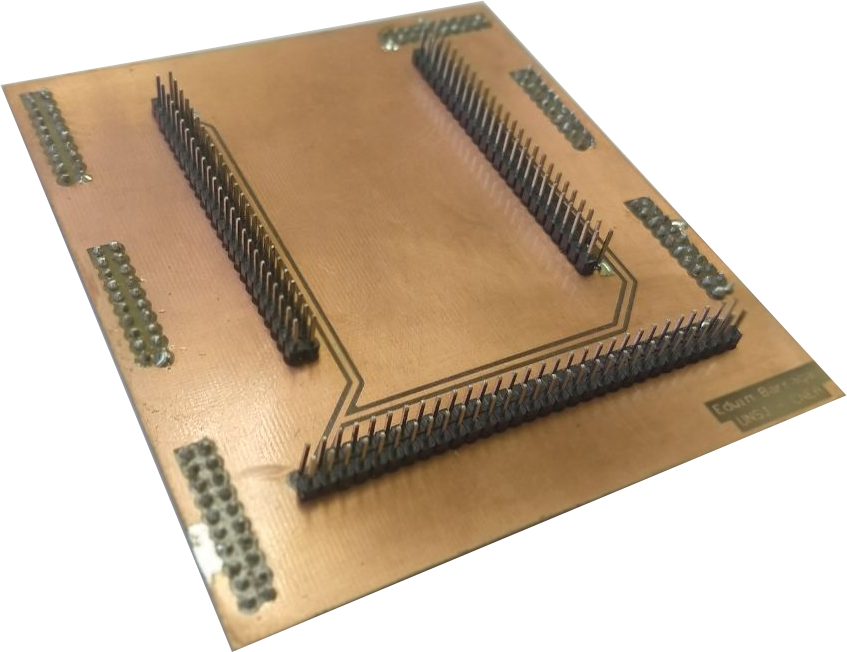
\includegraphics[width=.6\textwidth]{61v1anverso}}
			\only<2>{\centering
				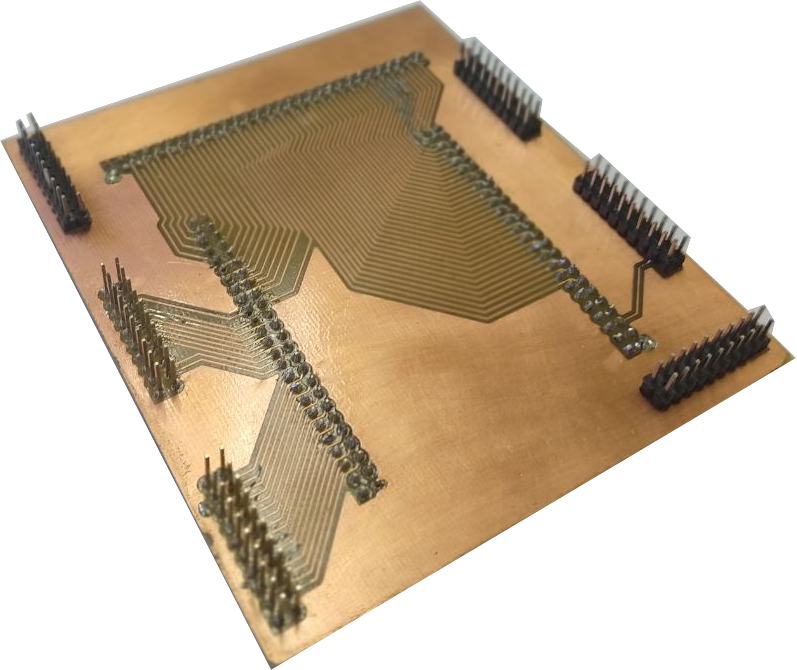
\includegraphics[width=.6\textwidth]{62v1reverso}}}
			
		\only<3-4>{\item Versión 2\\
			\only<3>{\centering
				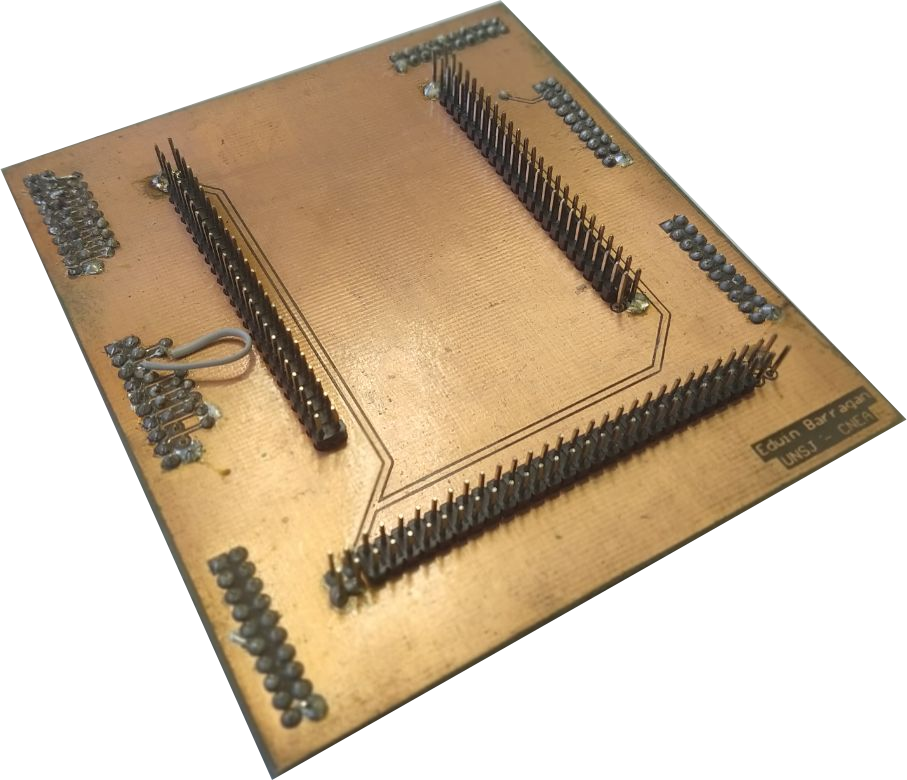
\includegraphics[width=.6\textwidth]{63v2anverso}}
			\only<4>{\centering
				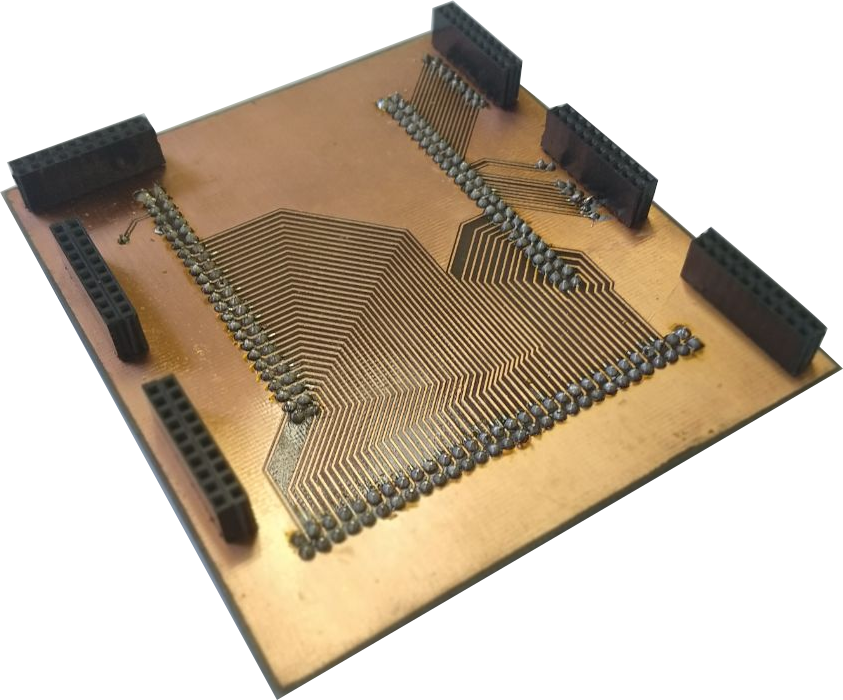
\includegraphics[width=.6\textwidth]{64v2reverso}}}

		\only<5-6>{\item Versión 3\\
			\only<5>{\centering
				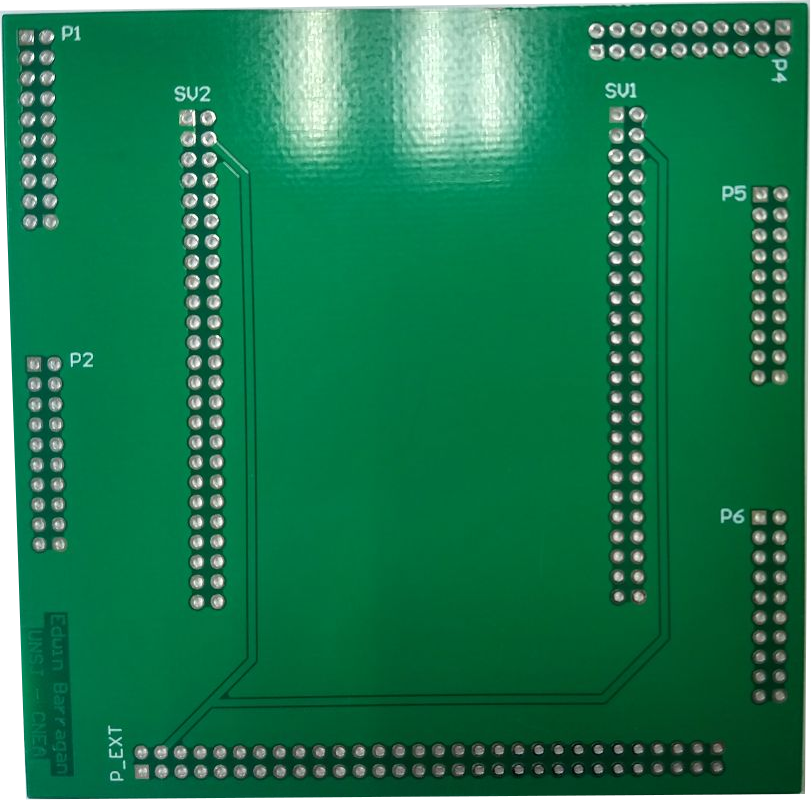
\includegraphics[width=.6\textwidth]{65v3anverso}}
			\only<6>{\centering
				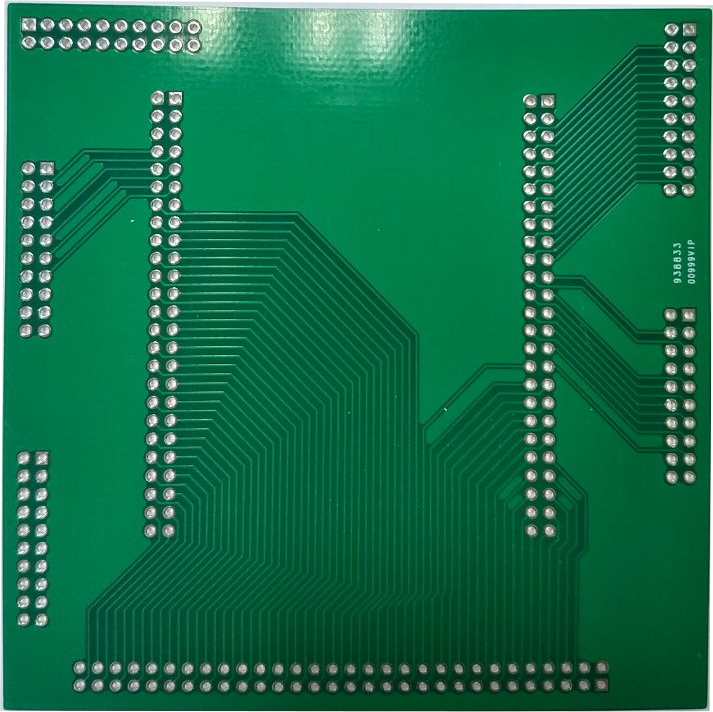
\includegraphics[width=.6\textwidth]{66v3reverso}}}
	\end{itemize}
\end{frame}
\begin{frame}{Sistema completo}
	\centering
	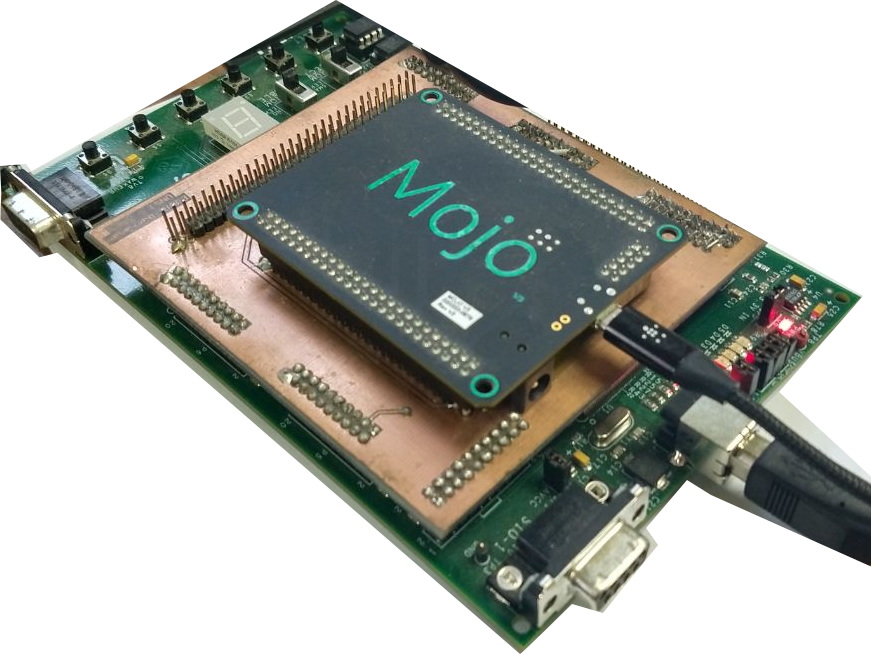
\includegraphics[width=.6\textwidth]{fisico}
\end{frame}

	\section{Evaluación y validación}
		\subsection{Desarrollo del sistema de pruebas}
			%\begin{frame}{Test bench}
%	\only<1>{El sistema fue simulado con el objetivo de corroborar el correcto funcionamiento del sistema, cómo así también detectar fallas en la descripción realizada y obtener una forma de depuración de lo realizado.}
%\end{frame}
\begin{frame}{Sistema de pruebas}
	\framesubtitle{Arquitectura}
	\centering
	\begin{tikzpicture}[scale=.53]
		\begin{scope}[transform shape,node distance=4,>=latex,double distance=1.3]
			\node[simple](mea)[]{Máquina de Estados Finitos};
			
			\node[simple,rounded corners](fx2lp)[left=of mea]{Interfaz EZ-USB FX2LP};
			\draw[<->,double]([yshift=10*220/11]fx2lp.south east) --node[above]{FD[15:0]}([yshift=220/11*10]mea.south west);
			\draw[<-,double]([yshift=220/11*9]fx2lp.south east) --node[above]{FADDR[1:0]}([yshift=220/11*9]mea.south west);
			\draw[->]([yshift=220/11*8]fx2lp.south east) --node[above]{FLAGA}([yshift=220/11*8]mea.south west);
			\draw[->]([yshift=220/11*7]fx2lp.south east) --node[above]{FLAGB}([yshift=220/11*7]mea.south west);
			\draw[->]([yshift=220/11*6]fx2lp.south east) --node[above]{FLAGC}([yshift=220/11*6]mea.south west);
			\draw[->]([yshift=220/11*5]fx2lp.south east) --node[above]{FLAGD}([yshift=220/11*5]mea.south west);
			\draw[->]([yshift=220/11*4]fx2lp.south east) --node[above]{SLWR}([yshift=220/11*4]mea.south west);
			\draw[->]([yshift=220/11*3]fx2lp.south east) --node[above]{SLRD}([yshift=220/11*3]mea.south west);
			\draw[->]([yshift=220/11*2]fx2lp.south east) --node[above]{SLOE}([yshift=220/11*2]mea.south west);
			\draw[->]([yshift=220/11*1]fx2lp.south east) --node[above]{PKTEND}([yshift=220/11*1]mea.south west);
			
			
			\node[simple,minimum height=150,minimum width=50](interno)[right=6 of mea.north east,anchor=north west]{Memoria FIFO};
			\draw[double,->]([yshift=-1*150/8]mea.north east)--node[above]{Dato\_enviado[15:0]} ([yshift=-1*150/8]interno.north west);
			\draw[double,<-]([yshift=-2*150/8]mea.north east)--node[above]{Dato\_a\_enviar[15:0]}([yshift=-2*150/8]interno.north west);
			\draw[<-]([yshift=-3*150/8]mea.north east)--node[above]{Enviar\_datos}([yshift=-3*150/8]interno.north west);
			\draw[<-]([yshift=-4*150/8]mea.north east)--node[above]{PKTEND}([yshift=-4*150/8]interno.north west);
			
			\node[simple,minimum height=70](adapt)[anchor=south] at  ($(mea.south|-interno.south)!0.5!(interno.south)$|-interno.south) {Adaptador};
			\draw[->]([yshift=-5.5*150/6]mea.north east)--node[above]{SLWR}([yshift=-5.5*150/6]mea.north east -| adapt.west);
			\draw[->]([yshift=-4.5*150/6]mea.north east)--node[above]{SLRD}([yshift=-4.5*150/6]mea.north east -| adapt.west);
			\draw[<-]([yshift=1*70/5]adapt.south east) --node[above]{Llena} ([yshift=1*70/5]adapt.south east -| interno.west);
			\draw[<-]([yshift=2*70/5]adapt.south east) --node[above]{Vacia} ([yshift=2*70/5]adapt.south east -| interno.west);
			\draw[->]([yshift=3*70/5]adapt.south east) --node[above]{wr\_en} ([yshift=3*70/5]adapt.south east -|interno.west);
			\draw[->]([yshift=4*70/5]adapt.south east) --node[above]{rd\_en} ([yshift=4*70/5]adapt.south east -|interno.west);
			
			\node[simple,minimum size=50](clk) [anchor=south]at (mea.south west-|interno.south)  {PLL};
			\draw[<-]([yshift=15]mea.east |- clk.west)--node[above,near end]{Reloj}([yshift=15]clk.west);
			\draw[->] (clk) -- node[right]{clk} (interno);
			\draw[->] ([yshift=15]clk.west) -| (adapt);
			
			\node[rounded corners,simple, minimum size=50](clkSrc)[right=1 of clk]{Fuente de reloj};
			\draw[->](clkSrc) to (clk);
			
			\node[simple,minimum size=30](rst)[anchor=south]at($(mea.south)!.5!(clk.south)$) {Reset};
			\draw[->]([yshift=15]clk.west)-|(rst.north);
			\node[simple,rounded corners,minimum size=50](puls)[below=1 of rst]{Pulsador};
			\draw[->](rst.west) --node[above]{Reset} (rst.west -| mea.east);
			\draw[<-](rst.south)--(puls.north);
			
		\end{scope}
		\begin{scope}[]
			\node[rounded corners,inner ysep=5pt,draw=blue,dashed,rectangle,fit={(clk)(mea)(interno)},label=north:\scriptsize{FPGA}](fpga){};
			\node[inner ysep=11pt, yshift= 8pt, draw=blue,dash dot,rectangle,fit={(puls)(fpga)(clkSrc)},label=north:\scriptsize{Mojo}](){};
		\end{scope}
	\end{tikzpicture}
\end{frame}

\begin{frame}{Sistema de Pruebas}
	\framesubtitle{Implementación en VHDL}
	\centering
	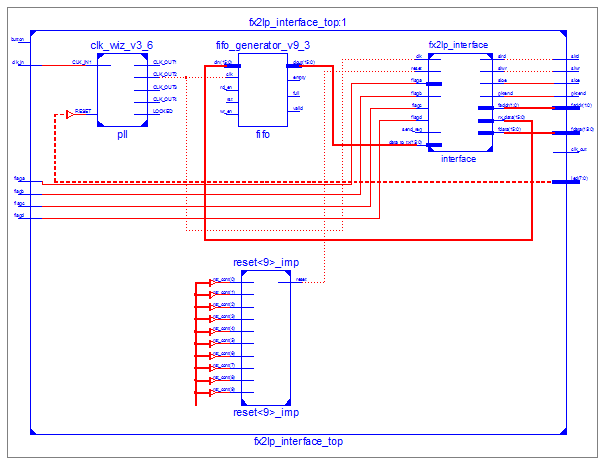
\includegraphics[height=.83\textheight]{fx2lp_rtl}
\end{frame}

\begin{frame}{Verificación Funcional}
	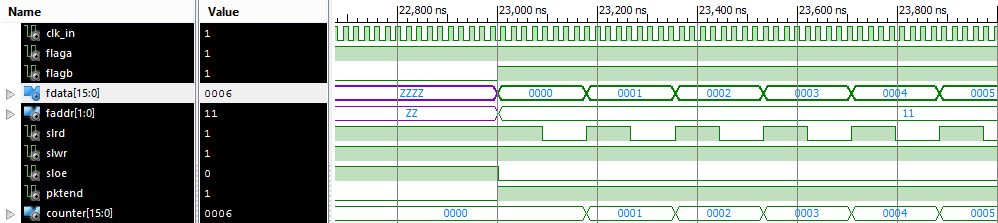
\includegraphics[width=\textwidth]{sist_tb_lect}
\end{frame}

\begin{frame}{Verificación Funcional}
	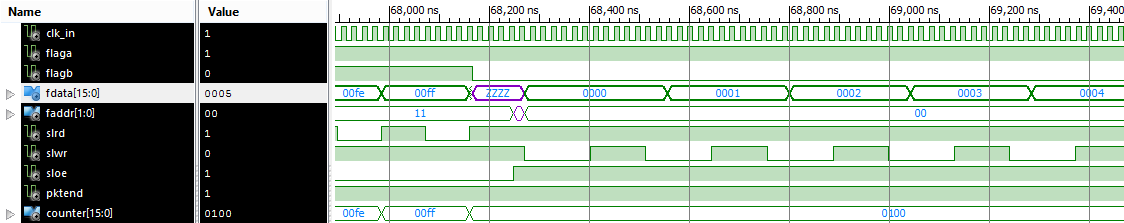
\includegraphics[width=\textwidth]{sist_tb_esc}\\
	\vfill
	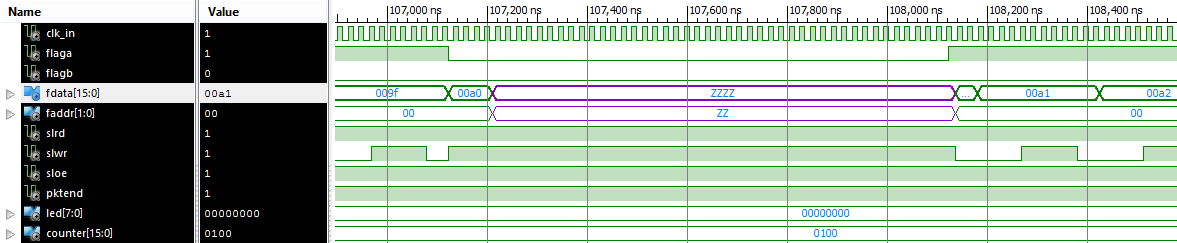
\includegraphics[width=\textwidth]{sist_tb_esc_int}
\end{frame}

\begin{frame}{Verificación Funcional}
	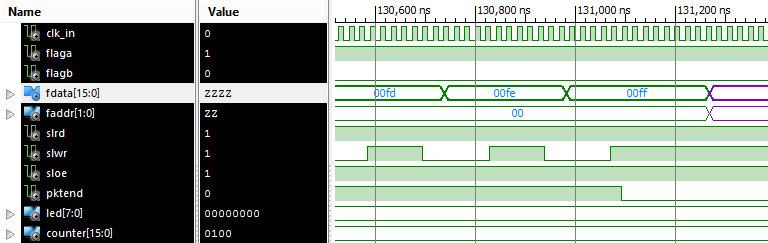
\includegraphics[width=\textwidth]{sist_tb_pktend}
\end{frame}
%\begin{frame}{Test bench - Lectura de la interfaz}
%	\only<1>{
%		\centering
%		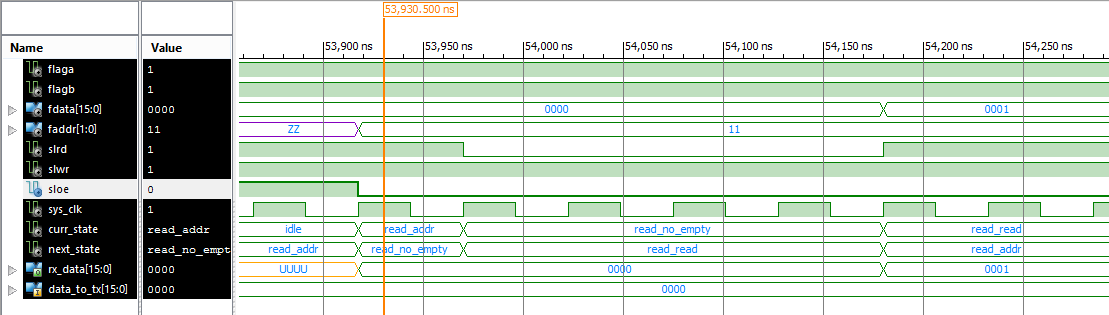
\includegraphics[width=\textwidth]{tb_if_rd_mef}\\
%		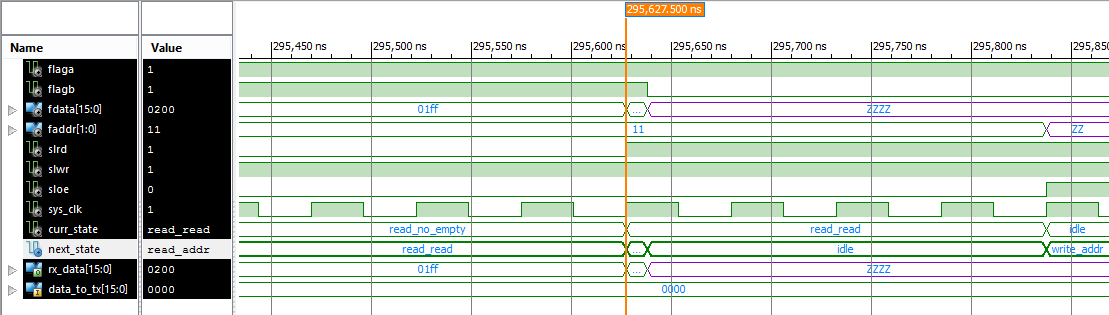
\includegraphics[width=\textwidth]{tb_if_rd_end}
%		}
%\end{frame}
%\begin{frame}{Test bench - Escritura en la interfaz}
%	\only<1>{
%		\centering
%		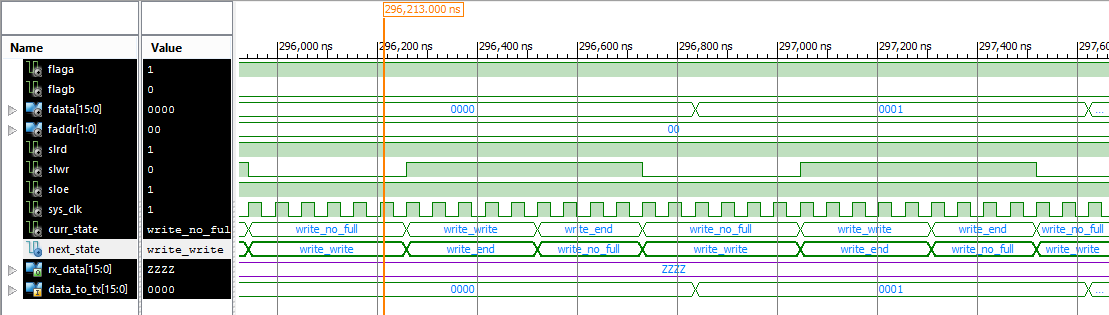
\includegraphics[width=\textwidth]{tb_if_wr_mef}\\
%		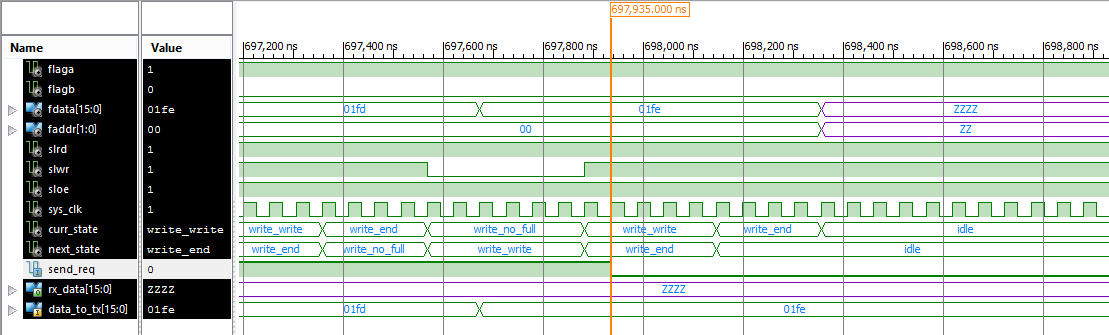
\includegraphics[width=\textwidth]{tb_if_wr_end}}
%	\only<2>{
%		\centering
%		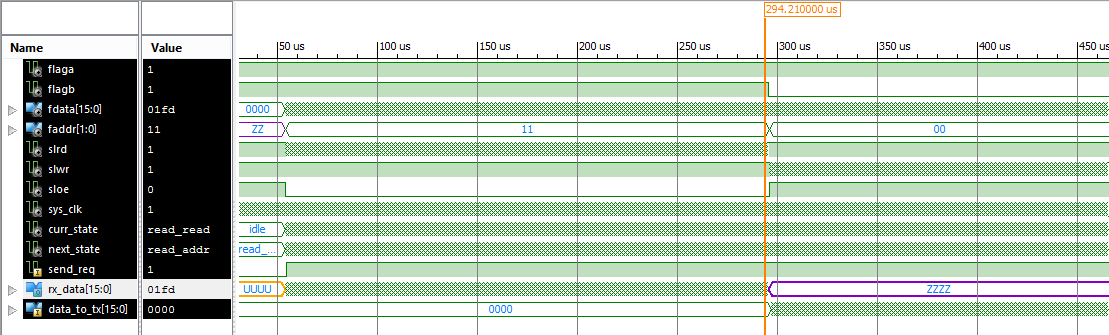
\includegraphics[width=\textwidth]{tb_if_snd}\\
%		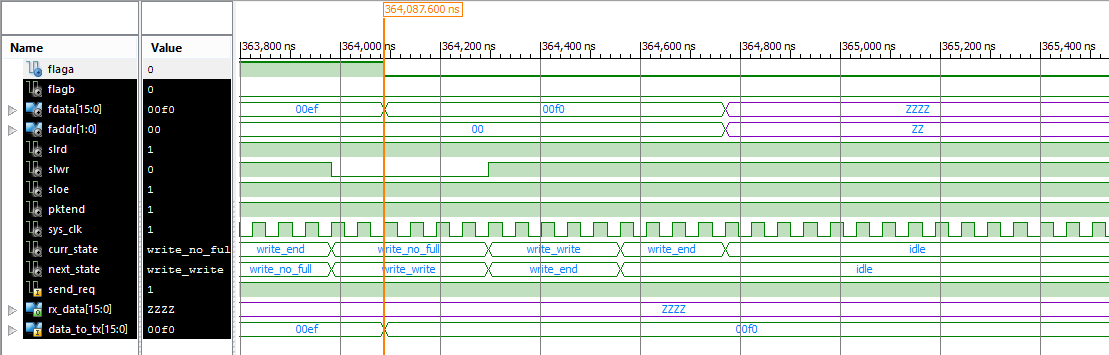
\includegraphics[width=\textwidth]{tb_if_fflag_end}}
%\end{frame}

%			\begin{frame}{Depuración de la interfaz en VHDL}
	\begin{itemize}
		\item Se utilizó un registro para elaborar un eco de a dos bytes. Permitió corroborar el correcto funcionamiento de la lectura y escritura de las memorias FIFO de la interfaz de Cypress.
		\item Se utilizó una memoria FIFO generada con el software ``Core Generator'' de Xilinx para lograr un correcto funcionamiento de las señales de la interfaz escrita en VHDL.
	\end{itemize}
\end{frame}

%		\subsection{Depuración de firmware del puente}
%			\begin{frame}{Debug Cypress}
	\begin{itemize}
		\item Se utilizó el framework provisto por Cypress para ser compilado con SDCC. No dió los frutos esperados.
		\item Se utilizó el framework provisto por Cypress para ser compilado con C51 de Keil. No funcionó en primera instancia.
		\item Se programó el puerto UART del 8051 para rastrear el error.
		\item Se logró que el framework trabaje adecuadamente solo con el puerto UART funcionando.
		\item Se utilizaron los LEDs indicadores para corroborar el llenado y vaciamiento de los extremos.
		\item Se aprovecharon los botones indicadores para corroborar el correcto funcionamiento de los extremos.
	\end{itemize}
\end{frame}

%		\subsection{Biblioteca de PC}
%			\begin{frame}{\texttt{libusb-1.0}}
	\begin{itemize}
		\item Se utilizó la biblioteca \texttt{libusb-1.0} para la elaboración de un programa de computadoras, escrito en C, que permita leer y escribir paquetes de datos desde la PC.
		\item Esta biblioteca es de código abierto y es soportada por todos los sistemas operativos actualmente en uso. Esto brinda la reutilización del código generado.
	\end{itemize}
\end{frame}

		\subsection{Desarrollo de un programa de pruebas}
			\begin{frame}{Esquemas de prueba}
	
\end{frame}

	\section{Resultados y conclusiones}
		\subsection{Pruebas y resultados}
			\begin{frame}{Resultados de la prueba de comunicación}
	\begin{itemize}
		\item El sistema envió y recibió paquetes durante 24 horas, logrando la correcta transmisión y recepción de 388.191.289 paquetes de 128 bytes cada uno.
		\item El sistema desarrollado estableció una comunicación USB de alta velocidad.
		\item La tasa de transferencia de datos es de 12,4 Mbps.
		\item No hubo perdida ni errores en los datos transmitidos.
		\item La tasa efectiva de transmisión de datos útiles fue de 9,12 Mbps.
	\end{itemize}
\end{frame}
		\subsection{Conclusiones}
			\begin{frame}{Conclusiones}
	\begin{itemize}
		\only<1>{
			\item Se desarrollo un sistema de comunicación USB 2.0 que permite conectar una FPGA con una PC. El enlace pudo ser operado a 480 Mbps.
			\item El sistema elaborado permite leer y escribir datos en forma robusta, es decir, sin perder datos.
			\item Se adquirieron y entendieron conceptos importantes de la norma USB 2.0.
			\item Se seleccionó y se configuró el controlador FX2LP como interfaz USB.
			\item Se seleccionó el FPGA Spartan 6 de Xilinx Inc, incorporado en la placa de desarrollo Mojo v3.
		}
		\only<2>{
			\item Se desarrolló una máquina de estados finitos implementada con el FPGA que comanda la comunicación entre este dispositivo y la interfaz USB.
			\item Se desarrolló un programa de computadoras que permite enviar y recibir datos a través del puerto USB.
			\item Se logró transmitir información desde y hacia la PC a una tasa efectiva de 9,12 Mbps.
		}
	\end{itemize}
\end{frame}

		\subsection{Trabajo futuro}
			El desarrollo expuesto en el presente trabajo puede ser de gran utilidad en el desarrollo de aplicaciones científicas. Se espera que el mismo sea utilizado en la lectura de imágenes adquiridas a través de sensores CMOS para aplicaciones tales como neutrografía y detección de radiación, entre otros.

Se plantea para trabajos futuros la posibilidad de implementar una nueva prueba de funcionamiento a través del envío ininterrumpido de tramas conocidas de datos, generados en forma local desde el FPGA, lo que permitirá conocer en mayor detalle la tasa máxima de bit posible con la configuración desarrollada en este trabajo.

Otra mejora a implementar en el sistema desarrollado consta de la realización sincrónica de la comunicación entre el FPGA y la Interfaz USB. Para ello, es necesario reconfigurar el controlador FX2LP, indicando que el funcionamiento de la memoria FIFO será de modo sincrónico. A su vez se debe rediseñar la placa de interconexión de forma tal que tanto el controlador FX2LP como el FPGA puedan compartir el reloj. Se espera que esta mejora brinde mayor velocidad al sistema, como así también se releve al FPGA de utilizar un PLL para brindar la señal de reloj necesaria, liberando recursos para su utilización en otro tipo de desarrollos implementados dentro de este.			
%			\begin{frame}{Material Adicional}
%			\end{frame}
%			\tiny{
%			\lstinputlisting[language=VHDL]{codes/fx2lp_interface.vhd}
%			\lstinputlisting[language=VHDL]{codes/fx2lp_interface_top.vhd}
%			\lstinputlisting[language=VHDL]{codes/fx2lp_interface_top.ucf}
%			\lstinputlisting[language=VHDL]{codes/interface_test_bench.vhd}	
%			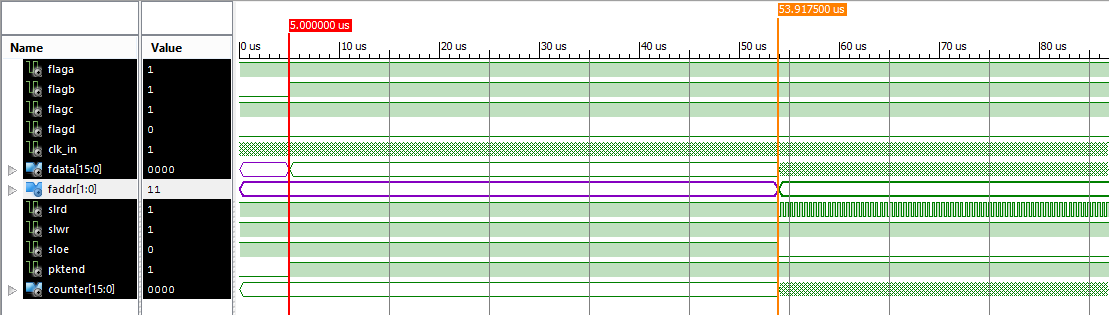
\includegraphics[width=\textwidth]{tb_top_sys_init}\\
%			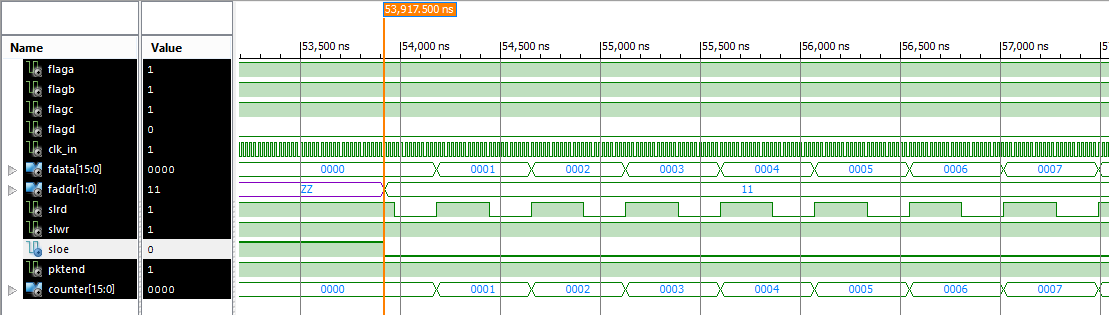
\includegraphics[width=\textwidth]{tb_top_rd_init}\\
%			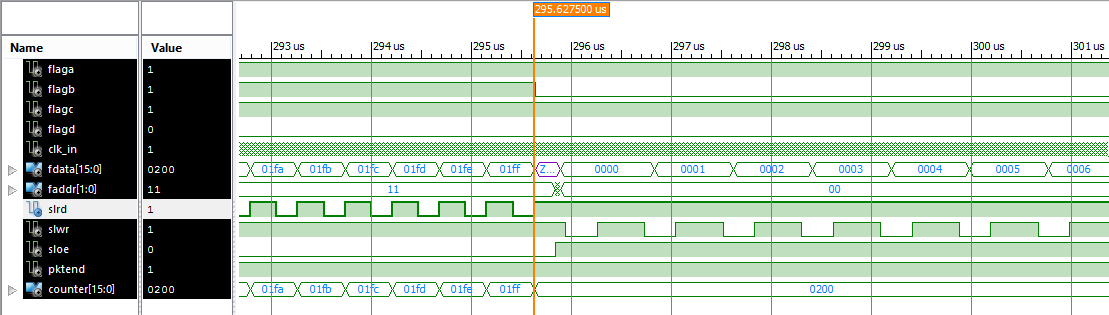
\includegraphics[width=\textwidth]{tb_top_rd_end}\\
%			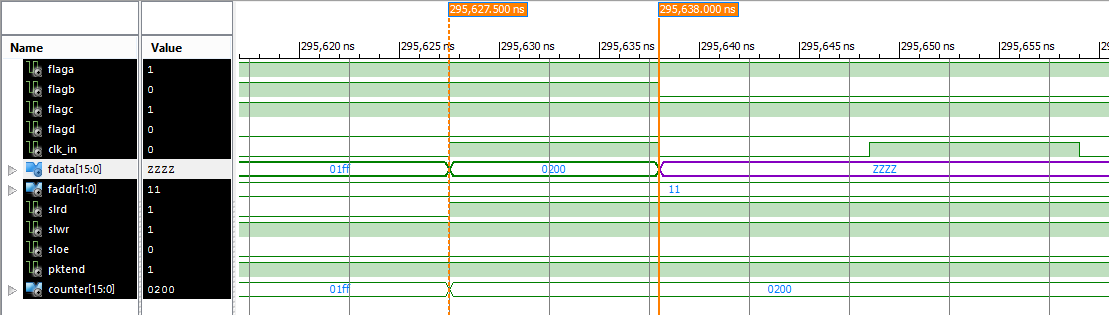
\includegraphics[width=\textwidth]{tb_top_rd_end_det}\\
%			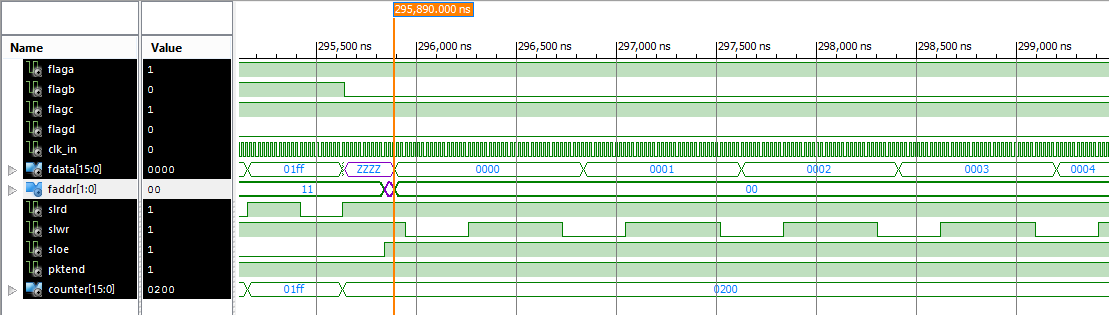
\includegraphics[width=\textwidth]{tb_top_wr_init}\\
%			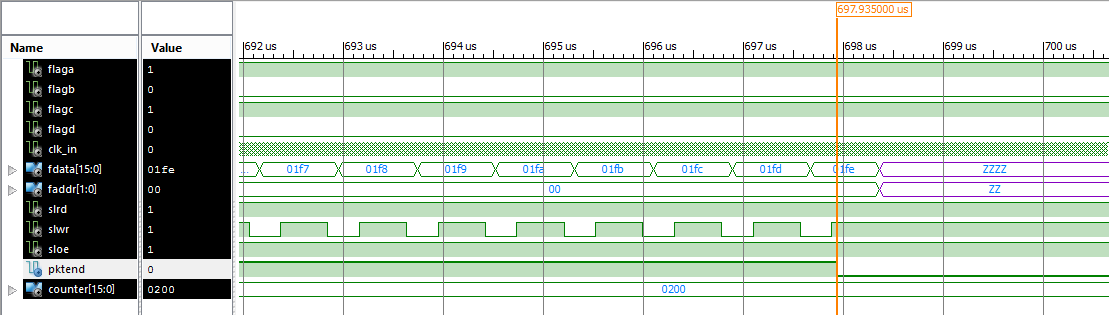
\includegraphics[width=\textwidth]{tb_top_wr_end}\\
%			\lstinputlisting[language=C]{./codes/bridge.c}
%			\lstinputlisting[language=C++]{./codes/tfUSBCheck.cpp}
%			\lstinputlisting[language=C++]{./codes/tfUSBCheck.h}
%			}
\end{document}